\documentclass{hautart}

\hautset{
    title = 计算机联锁培训系统设计,
    author = 张睿,
    gakubu = 电气工程学院,
    class = 轨道1702,
    stuid = 201712010311,
    teacher = 尚庆松,
    rank = 讲师,
    engtitle = Design of Computer-based interlocking edutraining system,
    date = 2021年5月15日
}
\usepackage{appendix}

\begin{document}
\pagenumbering{Roman}
\maketitle
\null
\begin{abstract}\normalsize
    车站连锁能够保证行车安全、提高运行效率,当下,在车站联锁系统中,
    计算机联锁已然成为主流。而计算机联锁培训系统就是用于计算机联锁教育培训的
    产品。而软件仿真则是最普遍的一种培训系统的模式。但传统的软件仿真计算机联锁
    培训系统存在着教学效率低、需要软件分发、软件运行环境限制、难以管理等问题。

    本设计使用IT行业内最新的软件设计技术,设计了一款基于Web、分布式、可扩展、
    高性能、高度灵活的计算机联锁培训系统,使用了极其高效的 Rust 程序设计语言,
    采用异步编程范式作为服务端,使用React.js和Two.js来渲染web端。
    设计为Web应用使得本设计不需要拘束于任何操作系统。
    并解决了传统软件计算机联锁培训系统的C/S模式的其他种种缺点,提高了培训效率。

    根据分布式的架构,本文使用了相应的技术来实现各层的各个模块,以及各个模块
    之间的耦合。在最后,对本设计进行了测试,以证明本设计实现了设计所要求的目标。
\end{abstract}
\textbf{关键字:} 分布式系统;Web应用;GraphQL;Rust程序设计语言;计算机联锁
\newpage

\twolines
\noindent\textbf{\large{Title}} ~ \uline{\large\hautengtitle\hfill}
\\
% \hangindent 4em \uline{\hautengtitle\hfill}

\renewcommand{\abstractname}{\flushleft\large{Abstract}}
\begin{abstract}\normalsize
    \noindent
    Computer-based interlocking has become the mainstream in station interlocking systems, which can ensure the safety of traffic and improve operational efficiency.
    The computer-based interlocking training system is a product used for computer-based interlocking education and training.
    Software simulation is the most common mode of training system. However, the traditional software simulation computer-based
    interlocking training system has problems such as low teaching efficiency, the need for software distribution, software operating environment restrictions,
    and difficulty in management.

    This design uses the latest software design technology within the IT industry to design a web-based, distributed, scalable, high-performance,
    and highly flexible computer-based interlocking training system that uses the extremely efficient Rust programming language,
    an asynchronous programming paradigm as the server side, and React.js and Two.js to render the web side.
    Designed for web applications makes this design not bound to any operating system.
    It also solves various other drawbacks of the C/S model of traditional software computer-based interlocking training system and improves the training efficiency.

    According to the distributed architecture, this paper uses the appropriate technology to implement each module of each layer and the coupling between each module.
    At the end, the design is tested to prove that it achieves the objectives required by the design.
\end{abstract}
\textbf{Keywords:} Distributed systems;Web application;GraphQL;Rust Programming Language;Computer-based interlocking
\newpage
\twolines
{
    \leading{18pt}
    \tableofcontents
}
\newpage

\pagenumbering{arabic}

%------------正文部分----------------%
\section{序论}
\subsection{研究背景与意义}
计算机联锁系统(CI)是综合运用计算机技术、网络通信技术和现代控制技术,
以电子信息传输方式集中操纵动力式道岔及色灯信号机等信号设备,从而实现控制车站的信号系统的功能的自动控制系统。
铁路车站是以建立进路的方式实现对列车、车列的运行控制。
计算机联锁系统通过计算机运算方式确保信号、道岔、进路间的相互关系正确,
满足各种车站、车场规模化运输作业的需要,能够保证行车安全,提高运输效率,改善劳动条件,
是车站信号设备控制系统的发展方向,是实现铁路现代化的重要基础之一。
联锁系统是铁路车站保证列车和车列正常和安全运行必不可少的核心基础设备。
而计算机连锁培训系统则是培训相关从业人员计算机连锁内容与相关操作的考试练习系统。
计算机连锁培训系统的目的在于:仿真模拟出现场的车站作业环境,能够达到练习、考试等培训功能,
通过练习功能、帮助学生深入学习计算机联锁,对计算机连锁的结构与操作工序逐渐的熟练,通过考试,
让教师能够对学生的水平有直观的判断与考察。提升计算机连锁教学的效率与品质。传统上,
计算机联锁培训通过视频教学、书本教学等培训手段,或者硬件模拟联锁逻辑实现,无法使仿真培训普及化以及并行化。
传统的计算机联锁教学相较于计算机联锁培训系统,更像是纸上谈兵,作为一门强实践性的技术,
计算机联锁培训系统能大大提高教育与学习的效率,已经是当今计算机联锁培训教育的首选教学工具。
若能结合联锁逻辑的纯软件模拟和web技术,则能让计算机联锁系统不再掣肘于空间与时间。
只要在可存取的互联网环境下,则可以处处进行计算机联锁的仿真学习。降低学习成本,提升学习效率。
摆脱了硬件仿真,则教学系统可以几近于零成本地部署在各处的服务器上,降低了安装部署的成本。
因此计算机联锁逻辑结合网络技术的应用,在计算机联锁培训领域内是十分重要的发展方向。

\subsection{国内外研究发展现状}
\subsubsection{国外现状}
国外对于计算机仿真培训系统采用了很多的技术手段来实现,因涉及很多学科,所以起步较早。
发达国家在上世纪八十年代就提出了相关的概念,并在十年内快速发展并取得良好的实用。
例如:英国铁路部门采用了计算机网络、计算机模拟器、信号模拟器等技术手段进行搭建系统,使用于模拟和培训;
美国主要采用计算机仿真技术、多媒体技术、网络技术等组成实训系统。
日本采用力学仿真及数据运算的同时还使用多媒体闭路电视进行直观培训。 

\subsubsection{国内现状}

在国内,计算机连锁培训系统主要分为以下三种形式:纯实物仿真培训、沙盘模拟仿真系统、纯软件的计算机联锁仿真培训系统。

纯实物仿真培训采用真实的信号机、钢轨、转辙器、轨道电路、列车等轨道交通信号设备作为仿真的表示层,
采用真实的计算机联锁软件进行仿真培训,这种培训方式的优点在于,最贴近实际作业环境,
能最真实的反应出学生在真实站场中可能遇到的各种场景和问题,表示直观,能体现出实际站场中信号设备和计算机联锁系统的耦合逻辑。
其缺点在于,成本耗费巨大,硬件调试困难繁杂,越复杂的车站便要越大的空间才能部署,培训难以并行化,车站毫无扩展性,
严重依赖硬件作为表示层,使培训流程严重受限于硬件状态。比如南京铁道职业技术学院内设有两个车站,相去1公里。

沙盘模拟仿真系统采用真实的信号机、钢轨、转辙器、轨道电路、列车等轨道交通信号设备作为仿真的表示层,
采用真实的计算机联锁软件进行仿真培训,这种培训方式的优点在于,拥有实物模型,能够直观的看到整个车站实际的状态,
比较贴近实际作业环境,占地面积小,整个车站只需要一间房间即可容下,相较于纯实物仿真而言成本低廉,但拥有纯实物仿真培训的大多数优点,此外,
由于可以将多个车站构建于一个沙盘上,每一个车站都能同时进行一人的培训。缺点:构建沙盘需要一定的成本,需要硬件调试,培训流程一定程度掣肘于硬件状态
,囿于列车的数量和位置,车站之间耦合性强,一个学生的培训流程会被其他学生的培训流程所影响,进而影响整个培训系统的效率。
整个系统能承载的学生和车站种类有限,可扩展性较差,如果沙盘上部署的车站不同,则无法进行标准化考试,只可作为练习使用。

纯软件的计算机联锁仿真培训系统采用完全软件模拟的表示层和联锁逻辑构建培训系统进行计算力联锁的仿真培训,
这种模式的优点在于没有任何的硬件电路,可用性强,可以通过升级软件等方式获得其他车站,而联锁逻辑是独立的通用模块无需更动,扩展性强,易于维护。
只需要计算机即可完成部署,不依赖大面积空间,成本低廉。不依赖硬件状态,可以不受限于其他车站的状态,软件可以复制,便于分发,
同一个车站可以分发给多个学生进行练习,能够实现并行化考试与练习,可以任意组合车站,不囿于物理的车站连接关系。易于设定权限组分别提升教师权限,
不掣肘于列车数量,可以随意增开列车排列进路。方便在考试前设定题目和评分标准,使所有学生同时使用相同的车站完成相同的任务方便标准化的考试,
产生有参考价值的考试成绩。

\clearpage
\section{需求分析}
uroj旨在设计一款高性能、可扩展、高并发、通用性计算机联锁培训系统。
通用性在于我们需要一款不拘束于某个具体车站的计算机联锁培训系统。本系统需要拥有对任意一车站进行
联锁培训的能力,可扩展性在于需要让用户可以自己定义车站。用户可以在自定义的车站上进行联锁培训,
并且要求定义过程简单易懂,不需要用户输入多余的内容。

若要满足这一点,传统的联锁表必然不符合,联锁表相当于枚举了整个车站的设备,车站规模越大,
联锁表就越复杂,而且如果要求用户上传联锁表用于联锁逻辑,则还要上传站场图用于渲染,但
显然的,站场图和联锁表描述的都是同一种事物--车站。由于这些问题,uroj选择了图论算法
来驱动联锁逻辑。而用户只需要编辑上传一个文件就能描述整个车站:包括各种设备之间的耦合关系
还有车站的地理布置。并使用这个车站来创建自己的计算机联锁模拟环境,这就是本设计的目标。


高性能在于作为一款web应用,尽量缩短相应时间、提升硬件利用效率,减少冗余。
高并发在于作为一款web应用,通过设计保证系统能够同时并行处理尽量多的请求。
\clearpage
\section{系统概览}
\subsection{系统架构}
为提高并发,提升应用性能,本案采用分布式系统设计,如图\ref{org} 所示,

\begin{figure}[htbp!]
    \centering
    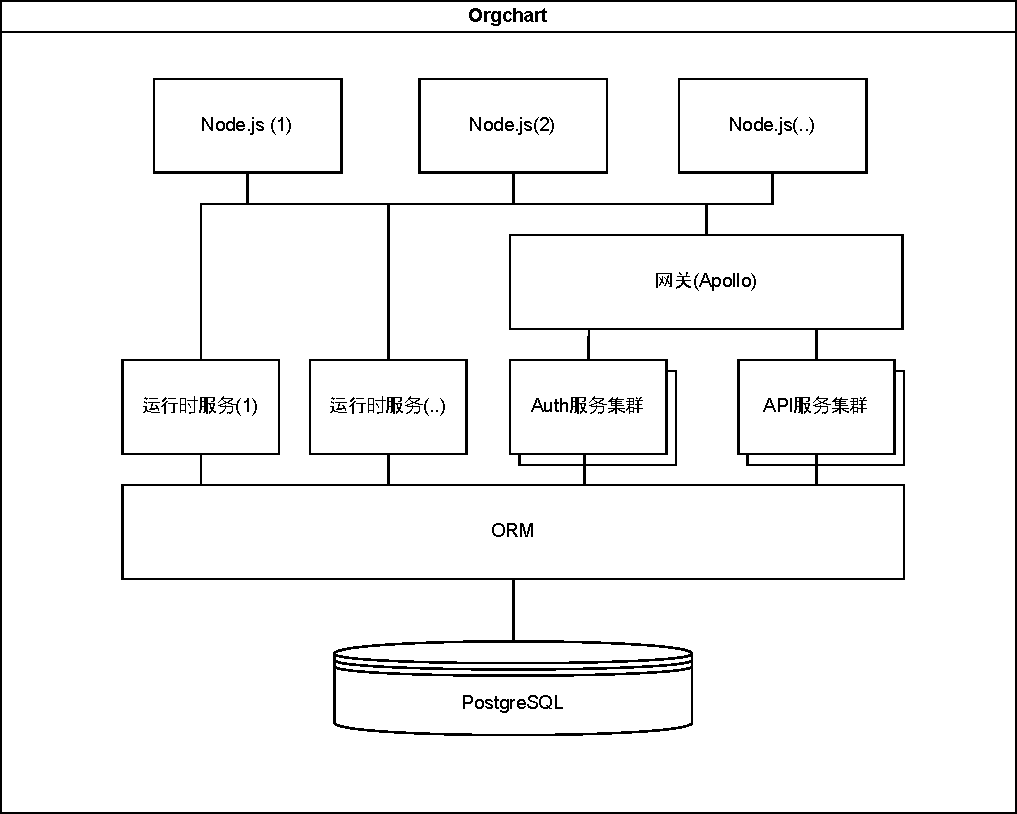
\includegraphics[width=0.95\textwidth]{figures/pdf/org.pdf}
    \caption{\label{org}系统架构组织图}
\end{figure}

本案符合非典型的web应用层次结构,分为表现层,接入层,业务逻辑层,数据访问层。
数据访问层采用名为 diesel 的 Rust crate 作为 ORM。
业务逻辑层分为Auth、API、Runtime等数个服务,每个服务都是独立的应用,可以横向扩展组成集群。
接入层使用 Apollo 作为 GraphQL 的网关,向外暴露所有的服务接口,还可以进行流量控制,但为了
支持运行时(Runtime)服务的“热插拔”,运行时服务并不会使用网关。
表现层使用 Node.js 作为 Web 的运行时,使用 React 作为 GUI 框架。
表现层和接入层、业务逻辑层使用 GraphQL 实现 Schema,使用 HTTP 和 WebSocket 协议通信,
并使用 actix-web 作为web服务端。


\subsection{生命周期与任务调度}
一个典型的练习实例生命周期由以下几部分组成
\begin{enumerate}[\indent i.]
    \item 创建车站
    \item 用户创建练习实例
    \item 初始化实例
    \item 访问实例
    \item 结束实例
\end{enumerate}

其中,创建车站就需要用到后文提到的车站描述文件,车站被创建后将存入数据库中。创建好车站后,就可以创建
这个车站的实例。实例是uroj的最终端功能,是用户与联锁逻辑交互的直接对象,也是uroj的业务核心。
一个用户的一次练习就是一个实例,一个用户的一次考试也是一个实例。

本案支持预约或称定时开始的实例,在开始之前若用户尝试在executor
初始化一个实例,就会报错。在GUI上,在开始时间之前,不渲染开始按钮,和后端的时间约束形成两层约束。
实例创建后同样也会被记录在数据库中,当时间到后用户就可以在创建实例时指定的executor上
初始化实例 -- executor从数据库中读入instance,并运行。
实例初始化后用户就可以在该实例中进行进路车辆的各种操作。
最后实例会被结束。

在uroj的架构中,runtime服务(后文也称为“执行器”)的作用是实例运行的容器。其提供了
实例运行所需要的环境(如联锁逻辑、车站拓扑关系分析等)一个容器可以同时让多个
实例在其中运行。因此得名运行时或执行器。正如上表所示,一个车站可以创造无限个实例,
这也是本设计通用性的一大体现。

一个典型的考试实例生命周期由以下几步构成
\begin{enumerate}[\indent i.]
    \item 创建车站
    \item 创建考题、考试
    \item 批量创建实例
    \item 初始化实例
    \item 访问实例
    \item 结束实例
\end{enumerate}

和练习实例不同之处在于,一场考试是有考题的。同一场考试中无论考试有多少,考题
都是相同的。通过班级结构,可以在配置考试实例时指定受验班级,系统自动为
班级所有的学生创建配置信息完全相同(即开始时间、结束时间、考题、车站等等)的实例。

本案正是通过对于考题、车站等配置信息的最高效复用以实现通用性的。
\clearpage
\section{业务层}

\subsection{API 服务}
API服务主要负责耦合data层和view层,上承用户的请求,下接数据库,从数据库读写数据并呈递给前端。
在本案中,API服务提供车站、实例、考试、用户和班级四个类型的服务。
在api服务中,Station 数据是最完备最上游的车站静态数据,其直接来源于用户的输入。Station 数据
直接来源于车站描述文件。

\subsubsection{车站}

在说明车站在api服务中如何被创建获取之前,让我们先解释一下什么是
车站描述文件以及其中的车站属性。

\paragraph{}车站属性

车站属性从性质上可以分为图形属性和逻辑属性,
图形属性用于表现层初始化Instance时正确地渲染出车站底平面图,
逻辑属性用于Runtime初始化实例时正确地描述车站的拓扑关系和耦合逻辑。

但车站的某个属性并非一定为图形属性或逻辑属性。本案特别地为此做出优化:
本案只需要输入可以独自或和其他属性一起提供渲染或联锁逻辑所需信息的车站属性。
也就是一个车站由完整描述车站的最小属性集合所描述,而之后业务中所需的所有信息都将由这个集合推导。
如此以来用户不必输入非必要的冗余信息,提升了用户体验。基本上,一个车站是由数个Signal和数个Node构成的,
所以,车站属性从组件上可分为Signal属性和Node属性。
表\ref{node_prop}中为Node的属性,
表\ref{sgn_prop}为Signal的属性。

这些信息保存在用户上传的车站描述文件中,并储存在数据库车站表(station)的yaml行内,
其会在运行时服务被反序列化成所需的各种对象。

\newcommand{\yes}{$\checkmark$}
\begin{table}[htpb!]
    \centering
    \caption{\label{node_prop}Node属性}
    \begin{threeparttable}
        \begin{tabular}{lccc}
            \toprule
            属性               & 作用         & 图形属性 & 逻辑属性 \\
            \midrule
            NodeID             & 唯一确定Node & \yes     & \yes     \\
            NodeKind           & 类型         &          & \yes     \\
            TurnoutID$^*$      & 所属道岔     &          & \yes     \\
            TrackID            & 所属轨道电路 &          & \yes     \\
            LeftAdj$^*$        & 左邻Node     &          & \yes     \\
            RightAdj$^*$       & 右邻Node     &          & \yes     \\
            ConflictedNode$^*$ & 抵触节点     &          & \yes     \\
            Line               & 渲染线段     & \yes     &          \\
            Joint              & 绝缘节类型   & \yes     &          \\
            \bottomrule
        \end{tabular}

        \begin{tablenotes}
            \footnotesize
            \item[$*$] 表示该属性有数个
        \end{tablenotes}
    \end{threeparttable}

\end{table}

\begin{table}[htpb!]
    \centering
    \caption{\label{sgn_prop}Signal属性}
    \begin{threeparttable}
        \begin{tabular}{lccc}
            \toprule
            属性          & 作用           & 图形属性 & 逻辑属性 \\
            \midrule
            id            & 唯一确定Signal & \yes     & \yes     \\
            SgnKind       & 信号类型       & \yes     & \yes     \\
            SgnMount      & 安装方式       & \yes     &          \\
            Pos$^\dag$    & 安装位置       & \yes     &          \\
            dir$^\dag$    & 左右朝向       & \yes     & \yes     \\
            side          & 上下两侧       & \yes     &          \\
            ProtectNodeID & 防护Node       & \yes     & \yes     \\
            TowardNodeID  & 朝向Node       & \yes     & \yes     \\
            Btns$^*$      & 信号机安按钮   & \yes     & \yes     \\
            JuxSgn$^\dag$ & 并置信号机     &          & \yes     \\
            DifSgn$^\dag$ & 差置信号机     &          & \yes     \\
            \bottomrule
        \end{tabular}

        \begin{tablenotes}
            \footnotesize
            \item[$*$] 表示该属性有数个
            \item[$\dag$] 表示该属性非必须(可省略)
        \end{tablenotes}
    \end{threeparttable}
\end{table}

\paragraph{}车站描述文件

车站属性并非直接存储于数据库之中,而是由用户编写成车站描述文件,将描述文件存储在数据库内。
车站描述文件用于描述车站,即使用上述属性来定义一个车站,
车站描述文件作为用户向本系统的输入,是用户唯一定义车站的方式,因此,
为兼顾可读性和文件体积需求,本案采用json作为车站的描述语言。
JSON(JavaScript Object Notation)是一种轻量级的数据交换格式。
它便于人类阅读和书写。对于机器来说,它很容易解析和生成。它是基于JavaScript编程语言标准ECMA-262第三版-1999年12月的一个子集。
JSON是一种完全独立于语言的文本格式,但使用C语族的程序员所熟悉的约定,包括C、C++、C\#、Java、JavaScript、Perl、Python和许多其他语言。
这些特性使JSON成为理想的数据交换语言。\cite{rfc7159}。

车站描述文件将在Executor中被解析成实例,与此相关的细节参见第七章。前文曾道
“基本上,一个车站是由数个Signal和数个Node构成的”,但车站描述文件中除了信号机和节点的定义之外,还有另外两个字段
其一是车站的标题,一般为站名,另一为独立按钮,譬如咽喉区设置的列车终端按钮LZA,这种按钮是不依附于信号机的,
因此需要单独定义,包括按钮的id,位置和其映射的节点。
这里给出一个非典型的车站描述文件作为例子并在注释中说明上述内容。
\lstinputlisting{codes/test.json}
显然上述文件中定义了一个站线节点、一架进站信号机、一架出站兼调车信号机。

\paragraph{}新建车站

新建车站是用户输入车站信息(上述提到的承载车站属性的车站描述文件和一些其他信息)并将其插入数据库的过程。
表现层通过调用api服务Mutation中的 create\_station 来创建新车站。新建车站时需要的输入的项见表 \ref{create_sta_in}

\begin{table}[htpb!]
    \centering
    \caption{\label{create_sta_in}创建车站输入}
    \begin{threeparttable}
        \begin{tabular}{lc}
            \toprule
            属性            & 含义         \\
            \midrule
            title           & 标题         \\
            description$^*$ & 说明         \\
            draft           & 是否草稿     \\
            yaml            & 车站描述文件 \\
            \bottomrule
        \end{tabular}
        \begin{tablenotes}
            \footnotesize
            \item[$*$] 表示该属性非必须(可省略)
        \end{tablenotes}
    \end{threeparttable}
\end{table}

\paragraph{}获得车站

获得车站是通过查询数据库,使用户取得车站信息的过程。
当表现层调用api服务 Query 中的 station 方法时,该方法会通过用户输入的station id在数据库中查找车站
从API服务中获得的车站返回车站的所有原始信息,
需要注意的是,该车站信息是表现层控制面板中用于获得车站列表、查看车站信息使用的。
不是在初始化实例时渲染车站平面图用的,渲染车站平面图用的是运行时服务的“查询车站布局”。

\subsubsection{实例配置}

\paragraph{}创建实例配置

Instance是Station的实例,在运行时中 Instance 需要 Station 数据进行初始化。
但要想创建Instance,还需要一些必要的信息,譬如Instance类型,Instance支持两种类型:
练习和考试,二者都需要一些描述该类型的详细内容,比如Instance需要和用户交互,
所以需要在创建实例时指定实例的用户、详细的输入项见表 \ref{create_ins_in}。

\begin{table}[htpb!]
    \centering
    \caption{\label{create_ins_in}创建实例输入}
    \begin{threeparttable}
        \begin{tabular}{lc}
            \toprule
            属性            & 解释     \\
            \midrule
            title           & 标题     \\
            description$^*$ & 注释     \\
            player          & 用户     \\
            station\_id     & 车站id   \\
            executor\_id    & 运行时id \\
            \bottomrule
        \end{tabular}
        \begin{tablenotes}
            \footnotesize
            \item[$*$] 表示该属性非必须(可省略)
        \end{tablenotes}
    \end{threeparttable}
\end{table}

实例用户和实例创建者不一定相同,在大多数练习场景中自然是相同的,但是在考试场景中,考试实例一般是由管理员(教师)创建给普通用户(学生)的。
因为本案是分布式架构,因此整个系统不一定只有一台 Executor,因此创建Instance时需要指定一个 Executor 以执行该Instance。
另外,用户创建实例是还需要为其指定标题与描述(可选)。

创建实例时可以选择是否指定开始时间,若不指定则缺省为即时开始。一般练习的场景中,实例是即时创建的,
但在考试的场景中,教师通常会提前配置好未来的考试。在创建实例时指定实例的开始时间(也必须指定结束的时间)。

当新建实例之后,API会为实例生成唯一的UUID,
UUID(Universally Unique Identifier)是用于计算机体系中以识别信息数目的一个128位标识符,
UUID根据标准方法生成,不依赖中央机构的注册和分配,
UUID具有唯一性,这与其他大多数编号方案不同。重复UUID码概率接近零,可以忽略不计\cite{rfc4122}。
因此UUID十分适合用在分布式系统数据表的主键。因为服务集群中即使有多个数据库、多个服务节点
也能保证某个实例的主键是世界上唯一的。uroj使用PostgreSQL的gen\_random\_uuid函数生成版本4的UUID\cite{group2020documentation}。

数据库实例表中还有一个状态属性,表示实例当前的状态,如表\ref{ins_state} 当创建实例配置时会缺省为 Prestart,
,在运行时初始化实例时会更新为Playing,当结束后会更新为Finished。

\begin{table}[htpb!]
    \centering
    \caption{\label{ins_state}实例状态}
    \begin{tabular}{lc}
        \toprule
        状态     & 含义   \\
        \midrule
        Prestart & 未开始 \\
        Playing  & 进行中 \\
        Finished & 已结束 \\
        \bottomrule
    \end{tabular}
\end{table}

\paragraph{}获得实例配置

和车站相同,这里获得的时实例的配置信息而不是实例信息。实例信息是供实例真正在运行时中运行的时候
用来进行联锁逻辑或者供给表现层渲染用的。而这里获得到的实例配置是用于在表现层的控制台
中呈现某个实例的配置、运行信息用的。

\subsubsection{运行时}
运行时比较简单,新建运行时只需要输入运行时的地址,获得运行时获得运行时的id和地址。

\subsubsection{用户}
api 服务中的用户只能用来获取,即从数据库查到一个用户的信息并返回。和Auth中定义的用户操作
不同,api服务中的用户只是为了在表现层控制台中现实用户的个人信息。不用于验证身份、鉴权。
也不能用于修改用户信息。

\subsubsection{班级}
用户是可选是否有班级属性的。班级可以创建或获取。创建班级只需要输入班级的名称。
\subsection{Auth服务}
本案设管理员和用户两种用户身份,不同的服务需要响应的权限才能运行
\subsubsection{JWT}
JSON Web Token(JWT)是一个开放标准(RFC 7519),用于创建具有可选的签名和/或可选的加密的数据,
其载荷持有JSON。token 使用私人秘密或公共/私人密钥进行签名。服务器可以生成一个包含用户身份和用户id的token,
并将其提供给客户端。然后,客户端可以使用该token来证明其身份。

本案的 uroj-common crate 中封装了JWT相关的函数,其claim定义为
\begin{lstlisting}
pub struct Claims {
    pub sub: String,
    pub exp: i64,
    pub role: String,
}
\end{lstlisting}

其中 sub 是用户ID,exp是token有效期(本案取1小时),
role是用户身份,当用户登入时,生成一个claim并将其编码成token。
在web端将该token存入cookie中,在之后的所有请求头中携带token进行访问,服务端就可以将token解码成claim,
从而得知用户id和用户身份,从而判断用户是否有请求该方法的权限。

这个过程可以很形象的理解成当学生或教师进入大学时发放相关证件(学生卡/教职卡),卡片上记录着持卡人的信息和其身份(学生/教师等)
在学校内需要验证身份的时候就可以使用证件来验证身份。token就是一种这样的证件,由服务端签发,由web端持有,在服务端需要
验证身份时使用的。

\subsubsection{用户}
在uroj中生成一个新用户有两种途经、一个是只能由管理员执行的创建用户(create\_user),另一个
是注册。是两种很常见的应用场景。

\paragraph{}创建用户
创建用户的用户输入如表\ref{user_in}。

\begin{table}[htpb!]
    \centering
    \caption{\label{user_in}创建用户输入}
    \begin{threeparttable}
        \begin{tabular}{lc}
            \toprule
            属性          & 含义     \\
            \midrule
            id            & 用户id   \\
            email         & 电子邮箱 \\
            class\_id$^*$ & 班级id   \\
            password      & 密码     \\
            role          & 用户角色 \\
            \bottomrule
        \end{tabular}
        \begin{tablenotes}
            \footnotesize
            \item[$*$] 表示该属性非必须(可省略)
        \end{tablenotes}
    \end{threeparttable}
\end{table}

api服务得到用户输入后,会使用bcrypte算法加密用户输入的password。并将用户信息和加密后的密码插入
数据库的users表中。

关于bcrypte:bcrypt是一个由Niels Provos以及David Mazières根据Blowfish加密算法所设计的密码散列函数,
于1999年在USENIX中展示\cite{bycrypto}。本案中bcrypt会使用一个加盐的流程以防御彩虹表攻击,同时bcrypt还是适应性函数,
它可以借由增加迭代之次数来抵御日益增进的电脑运算能力透过暴力法破解。本案中使用 12 次迭代。

\paragraph{}注册

注册用户的用户输入如表\ref{sign_up_in}
\begin{table}[htpb!]
    \centering
    \caption{\label{sign_up_in}注册用户输入}
    \begin{threeparttable}
        \begin{tabular}{lc}
            \toprule
            属性     & 含义     \\
            \midrule
            id       & 用户id   \\
            email    & 电子邮箱 \\
            password & 密码     \\
            \bottomrule
        \end{tabular}
    \end{threeparttable}
\end{table}

和创建用户不同,注册用户时缺省用户角色为USER、缺省没有班级。本案中管理员只能由管理员
建立或者从普通用户提权。注册用户需要在登录之后再加入班级。和创建用户一样,注册用户
也会使用bycrypt加密用户密码。

\paragraph{}登入

登入用户的用户输入如表\ref{sign_in_in}
\begin{table}[htpb!]
    \centering
    \caption{\label{sign_in_in}登入用户输入}
    \begin{threeparttable}
        \begin{tabular}{lc}
            \toprule
            属性     & 含义   \\
            \midrule
            id       & 用户id \\
            password & 密码   \\
            \bottomrule
        \end{tabular}
    \end{threeparttable}
\end{table}

登入时会使用bycrypt验证用户输入的密码是否正确,如果正确则会生成一个JWT以返回。
该JWT会被表现层记录并且在后续的请求中将token携带在HTTP头中。

\paragraph{}获得用户:从数据库查询一个用户并返回

\paragraph{}禁用用户:从数据库查询一个用户并更新其is\_active 字段为 false。
\subsection{运行时服务}
运行时是供实例执行的运行时(runtime)环境,一个运行时中可以执行多个实例,所有的实例会被管理在一个
HashMap 中。实例在初始化时被插入该HashMap,在结束时移除。

\subsubsection{实例(Instance)}
实例是运行时中运行的基本单位,运行时服务的含义就是运行实例的服务。
一个实例由某个车站所实例化而来,在运行时中和表现层可以直接与相应的实例进行交互。
若拿做菜作类比,车站是“菜谱”、实例是“菜肴”、“上菜”是实例初始化并运行,与实例交互就是“吃菜”
一台实例的生命周期如下图所示:

一台实例只有一个逻辑用户,这是显而易见的,现实中一台终端只能同时由一个人操作。但本案还支持管理员控制
和状态共享。管理员控制是允许管理员对任意一个运行中的实例进行最高权限的操作,包括普通用户的所有权限还有
设置隐患(故障),任意生成列车等不和现实逻辑但有益于提高教学效率的操作。

\subsubsection{状态对象}
状态对象是状态机的组件,由 Signal(信号机状态对象),Node(结点状态对象) 和 Train(车辆状态对象)组成,
状态对象中保存着相应车站信号设备的实时状态。

\paragraph{}信号状态

譬如,Signal 中的二元组 filament\_status 表征灯丝状态,灯丝状态可取表\ref{fila_state}。
Signal 中的 state 属性表征信号机点灯状态,其可如表\ref{sgn_state}所列。
\begin{table}[htpb!]
    \centering
    \caption{\label{fila_state}灯丝状态定义}
    \begin{tabular}{cc}
        \toprule
        状态   & 含义 \\
        \midrule
        Normal & 正常 \\
        Fused  & 熔断 \\
        None   & 空   \\
        \bottomrule
    \end{tabular}
\end{table}
\begin{table}[htpb!]
    \centering
    \caption{\label{sgn_state}信号机状态定义}
    \begin{tabular}{cc}
        \toprule
        状态 & 含义 \\
        \midrule
        L    & 绿   \\
        U    & 黄   \\
        H    & 红   \\
        B    & 月白 \\
        A    & 蓝   \\
        UU   & 双黄 \\
        LU   & 绿黄 \\
        LL   & 双绿 \\
        US   & 黄闪 \\
        HB   & 红白 \\
        OFF  & 灭灯 \\
        \bottomrule
    \end{tabular}
\end{table}

\paragraph{}结点状态

与信号的状态类似,结点状态枚举参见表 \ref{node_state},
但需要注意的是在程序中还定义了锁闭枚举(Lock),但Lock并不参与业务逻辑,
真正表征锁闭状态的是 Node 状态对象中的is\_lock 属性。
该Lock枚举仅仅用于当Node锁闭时序列化成为状态帧向表示层发送。
\begin{table}[htpb!]
    \centering
    \caption{\label{node_state}轨道区段状态定义}
    \begin{tabular}{lcl}
        \toprule
        状态       & 含义 & 轨道电路状态     \\
        \midrule
        Vacant     & 空闲 & 调整             \\
        Occupied   & 占用 & 分路             \\
        Unexpected & 异常 & 断轨、分路不良等 \\
        \bottomrule
    \end{tabular}
\end{table}

结点状态可以由用户输入和车辆运动两种事件决定,相较信号状态更复杂一些,
因此用状态转移图来表示,如图 \ref{node_fsm}(不考虑非理想状况,如司机冒进信号):

\begin{figure}[htpb!]
    \centering
    \begin{tikzpicture}[font={\small}]
    \tikzset{
        ->, % makes the edges directed
        >=stealth, % makes the arrow heads bold
        node distance=4cm, % specifies the minimum distance between two nodes. Change if necessary.
        every state/.style={thick}, % sets the properties for each ’state’ node
        initial text=$ $, % sets the text that appears on the start arrow
    }
    \node[accepting,state] (A)               {$\{0,0,0\}$};
    \node[state]         (B) [right of=A] {$\{0,1,0\}$};
    \node[state]         (C) [right of=B] {$\{1,1,0\}$};
    \node[state]         (D) [below of=C] {$\{0,1,1\}$};
    \node[state]         (E) [left of=D] {$\{0,0,1\}$};

    \path (A) edge[above]              node {锁闭} (B)
    (B) edge[above]                node {车辆驶入} (C)
    (C) edge[right]                node {车辆驶出} (D)
    (D) edge[below]                node {自动解锁} (E)
    (B) edge[bend left, below] node {手动解锁} (A)
    (E) edge[left] node {锁闭} (B);
\end{tikzpicture}
    \caption{\label{node_fsm}结点状态转移图}
\end{figure}

其中状态变量\{a, b, c\}分别为:a: 0为vacant、1为occupied、2为unexpected, b: 是否锁闭 c: 是否曾占用
。图中未绘出异常状态,但,图\ref{node_fsm} 中的任意一种状态均可发生异常从而使node状态变为 unexpected.

\paragraph{}车辆对象

Train 中除了有id属性外,还有以下两个属性:

past\_node:其记录着一列车辆所历经的结点。用于解锁区段结点以及判断考题得分。
车辆对象可以自动的行进,如同一个完美的司机。

process:不大于1的浮点数,表示车辆在当前结点的进程,
比如 0.5 表示车辆位于当前节点正中


\subsubsection{实例组成}
一个实例基本由 fsm、topo、layout 三个独立的部分构成。
在实例初始化时会通过Station信息同时生成这三个部分。

\paragraph{}topo

topo 保存一个实例所有的拓扑关系,包括车站图(即联锁关系,包含$R$关系和$S$关系),并置信号机映射,差置信号机映射,以及独立按钮映射,
topo 能表征一个实例的各种组件(信号机、节点和按钮)在联锁逻辑上是如何耦合的。比如$R$关系表示了轨道结点之间
是怎么连接的\cite{石擎宇2014基于图论的联锁程序的研究与设计}。

通过topo,运行时可以静态地从车站的拓扑关系上找到一条可能的进路。再通过后续的判断,来确定这条可能的进路是不是
进路。

\paragraph{}状态机(FSM)

FSM(finite-state machine)即有限状态机, 保存了一个实例所有的状态对象,包括上述的信号机、节点和车辆,并且管理
整个车站的状态。后文将能改变FSM状态的因子称为事件(Event),而每发生一个事件,都有可能会导致
实例向表现层发送一个状态帧。

\paragraph{}布局(Layout)

实例中的布局对象是车站布局的载荷,即在用户请求车站布局时向表示层发送的车站布局信息。
布局在实例初始化时会和状态机同时生成,实际上,关于表现层的车站布局信息有两种方案,其一是不在初始化实例时在实例中储存布局信息
而在用户请求车站布局时再计算得出。其二是本案采用的,在实例初始化时同步计算布局信息并保存,当用户请求时直接返回布局信息。
这样做的好处是,以空间换时间,若有大量用户同时访问一个实例,或一个用户多次访问一个实例(如刷新页面),表现层请求车站布局用来渲染
车站平面图时,多次计算布局信息会造成不必要的时间开销。
一个布局由一组结点布局对象(NodeData)、一组信号布局对象(SignalData)和一个标题构成,标题用于渲染车站名。
NodeData和SignalData 用于渲染结点和信号机。

\begin{table}[htpb!]
    \centering
    \caption{\label{node_data}结点布局对象结构}
    \begin{tabular}{lc}
        \toprule
        属性       & 作用         \\
        \midrule
        NodeID     & 唯一确定Node \\
        TrackID    & 所属轨道电路 \\
        LeftP      & 左端点       \\
        RightP     & 右端点       \\
        LeftJoint  & 左端绝缘节   \\
        RightJoint & 右端绝缘节   \\
        \bottomrule
    \end{tabular}
\end{table}

\begin{table}[htpb!]
    \centering
    \caption{\label{sgn_data}信号布局对象结构}
    \begin{tabular}{lc}
        \toprule
        属性          & 作用           \\
        \midrule
        id            & 唯一确定Signal \\
        SgnKind       & 信号类型       \\
        SgnMount      & 安装方式       \\
        Pos           & 安装位置       \\
        dir           & 左右朝向       \\
        side          & 上下两侧       \\
        ProtectNodeID & 防护Node       \\
        Btns          & 信号机按钮     \\
        \bottomrule
    \end{tabular}
\end{table}

\paragraph{}考试管理器(ExamManager)

考试管理器是可选属性(Option),若且唯若实例为考试实例时才会有此属性,管理考试题目、考试进度以及考试分数
相关的内容。一场考试包含数个题目,考试管理器在考题被完成、跳过、超时的时候,会向表现层发送状态帧,供GUI
显示相关的考试进度,对于每一道考题在数据库中是由题目外键和实例外键构成的联合主键,意即即使对于参加
同一场考试的不同用户,其题目是相同的,对于一道相同的题目,可能有会出现在很多名用户的考试管理器中。
通过实例id和题目id,可以唯一的确定一个实例中的一道考题。考试管理器也可以凭此将用户的成绩信息上传
至数据库中。详细的数据结构可以参见第六章。

\subsubsection{获取实例信息}
表现层(用户)能从实例上取得的信息,有布局信息、考题信息和状态信息三种,布局信息和考题信息是静态的、
一次性的。而状态信息是实时的,动态的。布局信息用来正确地绘制车站的布局,考题信息用于向用户下达考试实例的题目,
状态信息用来更新车站上信号设备的状态。布局信息透过布局对象(layout)来传递,考试信息通过考试管理器发送,
状态信息透过状态帧(GameFrame)来传递。

uroj的运行时,无论在哪一层,布局和状态都是无耦合的。这意味着表现层需要单独地查询车站的布局和订阅实例状态
的更新。

\paragraph{}查询车站布局(Query Station Layout)

下面将介绍运行时是如何将上述的布局信息呈递给表现层的,而我们将在第九章看到如何利用表 \ref{node_data}
和表 \ref{sgn_data} 中所列之属性在网页上正确地渲染出车站平面。

运行时提供的车站布局接口是 station\_layout 方法,该方法会返回一个请求车站的layout的副本。当请求该
方法时,需要一个传入一个字符串作为id(UUID)参数,用来指明所请求的layout是哪个实例的layout,
运行时会在当前运行的实例中寻找用户所输入的id所对应的实例,
如果没找到则说明输入的id不是某个正在运行的实例。
如果找到了则把该实例的layout克隆并返回。

\paragraph{}查询全局状态(Query Global Status)
在表现层渲染车站布局后订阅状态更新前,需要先更新一次全局状态,运行时提供的车站布局接口是 global\_status 方法,

订阅状态更新后表现层会不断的获得实例的最新状态变化。但也仅限于状态变化,因为如果没有一些途径让
表现层得知订阅状态更新时的初始状态,就不能正确地表现整个车站的所有状态。
因此在获取车站布局时表现层时会同时请求一个全局状态,用来渲染请求状态更新时车站的初始状态,
后续订阅得到的状态更新都是在这个初始状态之上的状态改变。


\paragraph{}查询考题信息(Query Instance Question)

若且唯若实例为考试实例时(即实例的考试管理器不为空),表现层会查询实例的考题信息,考题信息

\paragraph{}订阅状态更新(Subscribe Status Update)

为保证表现层的状态能实时的被更新渲染,状态更新应该是长连接的单向流,uroj采用了graphql 的 subscription。
其能通过websocket 协议源源不断的向订阅者(表现层)发送数据。

状态帧(GameFrame)即是状态更新的载荷(Payload),即在需要更新表现层车站状态渲染的时候向
表现层发送的“新状态”,譬如某个信号机的灯光颜色,某个车辆的新位置,考试题目的完成,等等。
但不是所有的事件都会导致产生并发送状态帧,譬如轨道曾占用是用于解锁逻辑判断使用的,而不需要在视图上有任何表示,
所以轨道曾占用就不会产生状态帧。

状态帧目前分为6种,如表\ref{gameframe} 所示。

\begin{table}
    \centering
    \caption{\label{gameframe} 状态帧定义}
    \begin{tabular}{lc}
        \toprule
        状态帧 & 含义 \\
        \midrule
        UpdateSignal & 更新信号 \\
        UpdateNode & 更新节点 \\
        UpdateGlobalStatus & 更新全局状态 \\
        MoveTrain & 车辆移动 \\
        UpdateQuestion & 更新考题 \\
        InstanceFinish & 实例结束 \\
        \bottomrule
    \end{tabular}
\end{table}

其中UpdateSignal和UpdateNode分别包含id和state两个属性,
表示更新设备的id和新状态。UpdateGlobalStatus则是UpdateSiganal和UpdateNode的数组。
而MoveTrain有id属性表示被移动车辆的id,node\_id属性表示车辆所处的结点编号,process属性,表示车辆在当前节点的位置
,为小于1的浮点数,指的是车辆相对于结点的进程(即车辆走过了node\_id 结点的百分之几)。这些属性是与Train状态对象的
属性相同的,另外为了正确的渲染车辆的位置,MoveTrain状态帧还有一个属性名为 dir,意思是方向。结合process就能知道
此时车辆是在结点从左到右百分之几还是从右到左百分之几的位置处。
UpdateQuestion 只有当实例为考试实例时才会被发送,可以将某个编号的考题更新至:已完成、已超时、已跳过三个状态。
另外,和前四种状态帧不同的是,前四种状态帧是由状态机发送的,而更新考题状态帧是由考试管理器发送的。

状态更新的接口是 game\_update 方法,该方法会返回一个内容为GameFrame(状态帧)的流。
其中,当有需求一次性重置整个实例时,UpdateGlobalStatus这个状态帧会发送,该状态帧的内容其实就是前文提到的
更新全局状态的内容。

可能会发现,前文所定义的状态帧中的状态都只包含了新状态,而没有包含旧状态。这和某些事件驱动应用中的“事件”
不同。在本案中,表现层对于状态更新的策略是乐观的。意即表现层总是认为:自己接收到的状态帧中包含着最新的
状态。因此状态帧中不需要加入旧状态或者时间戳以保证状态变化的连续。

\subsubsection{实例初始化与运行}
无论用户是想要进行前文提到的请求车站布局(layout)亦或者是更新车站状态,最大的一个前提是实例要处于运行状态。
这是理所当然的,就像你不能品尝到一碟没有上菜的菜肴一样。你需要先让实例加载并运行在运行时内,才能获取
实例的车站布局或者更新实例状态。

在第五章,我们能够在api层中定义一个实例,预约实例运行的时间、配置实例相关的信息,并将这些信息存在数据库的
Instance 表中,那么在实例所指定的运行时 上,就可以运行该实例。要想运行实例。用户
需要输入实例ID(UUID)。而后运行时会通过数据访问层(uroj-db)在Instance表中查找相应的实例。
如果未找到,则说明访问的实例ID不合法。如果寻到对应的实例,则会验证实例的相关信息:如果访问实例
的用户没有权限(没有Guest、Player或Operator 权限),则返回forbidden禁止访问。若用户有权限。那么
还需要验证开始时间。因为在表现层,未满足开始时间要求的实例根本不会渲染开始入口(相关按钮),这里的
验证看似冗余而没有必要,但其实不然,uroj的各个模块间的耦合策略是悲观的,意思是,运行时 不应该信任
前端(表现层)传来的数据一定不会包含违反开始时间约束的实例访问请求。

当一切验证完成,运行时 便会将 yaml 反序列化成 RawStation 对象,用数据库中查到的实例信息,和RawStation
对象在运行时中新建实例。在这个过程中,Instance 的new方法会将传入的RawStation 转化为 fsm, topo 和 layout。

下面说明其中某些属性的推导过程,首先给出一个定义和一个推论:
\begin{definition}
    对于一个信号机,我们称其朝向的结点为该信号机的朝向结点,称其背向的结点为该信号机的防护结点
\end{definition}
\begin{corollary}
    某个信号机的朝向等于其所防护区段的端,相反于列车行进方向和其防护区段相对信号机的位置。
\end{corollary}
举例说明:

\begin{figure}[htbp!]
    \centering
    \begin{tikzpicture}[font={\small}]
    %uncomment if require: \path (0,300); %set diagram left start at 0, and has height of 300

    \draw    (0,-0.3) -- (0,0.3) ;
    \draw    (-3,0) -- (3,0) ;
    \draw    (0,0.5) -- (0,1.5) ;
    \draw (0.5,1) circle (0.5);
    
\end{tikzpicture}

    \caption{\label{ens1}例子}
\end{figure}

上述信号机朝\uline{左},因此其左边的结点为该信号机的朝向结点,右边的结点为其防护结点,并且,
该信号机防护其\uline{右}侧区段的\uline{左}端,限制来自\uline{右}行的调车。有了这个推论
便可以由原始数据推导出下列信息。

\paragraph{}信号机布局对象的位置和朝向

应该能注意到表\ref{sgn_prop} 中的 Pos 和 dir 属性是可选的。这是因为其中的pos和dir是缺省值。
即信号机的位置和朝向是可以从其他信息中推断出来的,这两个值如果留空则自动推断,如果不留空则
有限使用pos和dir作为信号机的位置和朝向,那么应该如何推断呢?

一般情况下,信号机位于两个轨道区段的衔接处, 绝缘节的旁边,因此通过表\ref{sgn_prop}定义的ProtectNodeID
和 TowardNodeID 可以找到信号机所对应的防护结点和朝向结点,那么由推论1必然有信号机的朝向
为从防护结点到朝向结点的方向,如果防护结点和朝向结点邻接(即在r关系中存在防护结点到朝向结点的边)
那么在有向图r中就能得知信号机的方向。换言之如果防护结点和朝向结点不邻接,则说明违反了定义1,
说明车站描述文件出错。

对于信号机的位置而言是同理的,由推论1,若信号机朝左则一定位于防护节点的左端点,若其朝右
则一定位于防护结点的右端点。而左端点或右端点的坐标是在RawNode(见表\ref{node_prop} )
中定义的。

\paragraph{}结点状态对象的防护信号机

对于FSM的结点状态对象来说,需要知道一个Node的左端信号机和右端信号机,
(这里需要明确一点:Fsm的Node状态对象中的左右端信号机,都应指的是防护本结点的信号机。)
可以通过RawStation在信号机上定义的防护结点,结合信号机的朝向就可得知:由推论 1
若信号机朝左,则其防护结点的左端信号机是该信号机,若信号机朝右,则其防护结点的右端信号机
是该信号机。

\subsubsection{结束实例}
相比实例的运行,结束实例要简单得多。结束实例分为两种,自动结束和手动结束。
对于考试实例而言,可以自动结束或手动结束。对于练习
实例则只能手动结束。对于考试实例而言,结束实例时会将考试管理器(ExamManager)的问题成绩
同步至数据库 instance\_questions 表中。对于练习实例没有什么额外的操作。

因为实例保存在HashMap中,因为rust语言的所有权和强制RAII的特性,所以不需要对实例进行析构。
只需要将Instance从HashMap中删除就可以结束实例。

在结束实例之后,会发送一个实例结束状态帧,以在表现层提示用户实例的结束。

\subsubsection{新建进路}
在详细说明建立过程之前,需要强调的一点是,新建进路过程的一个重要的性质为原子性:
和取消进路的分段过程不同,建立进路时必须保证所有轨道节点要么全部锁闭,
要么全部不锁闭(建立失败),不能出现部分节点锁闭部分结点不能锁闭的情况。

若不考虑竞态条件(多线程时),先检测一个可能进路中所有节点是否满足封闭条件,
再决定条件不满足而建立失败或者对所有结点统一进行锁闭以及对其进路扩展集进行征用。

若不事前检测进路锁闭条件,则需要在封闭结点到中途遇到无法锁闭之结点时对之前锁闭的所有结点
进行回滚(Rollback)。事实上,数据库事务的原子性便是通过这种方案保证的。但本案出于建立进路
的性质考量,采用第一种方案。

本案采用了为培训系统改良的新建进路算法,新建进路可以分为几个过程:查找结点、寻径、
进路约束检查、进路条件检查、封闭区段、点灯。

\paragraph{}查找结点

本案排选进路的核心算法以始终结点为输入,但实际上用户的输入却是按钮,如此一来
程序便需要从用户的输入得知用户真正想要建立的进路是从哪一个结点到哪一个结点的。

前文可知本案所定义的按钮有两种,一为信号机按钮,二为独立按钮。独立按钮自然有其到某个结点的映射。
但信号机按钮所映射的实体是信号机,而信号机有两个属性都和结点相关(防护结点和朝向结点)。那么
当用户点击信号机按钮时,究竟哪个结点才是用户想要建立进路的起点,哪个结点才是终点呢?

不难发现,对于起点来说,不论建立哪种进路,起点总是始端信号机的防护结点。
真正有问题的是终点的判断。不同类型的进路其终点和终端信号机的相对位置不同,就算是同种类型的进路,
若终端信号机有并置或差置,位置就又有不同。

枚举所有种类的进路,可以总结出终端结点的规律见表\ref{route_end}。

\paragraph{}寻径

在站场中查找路径本案中采用了petgraph这个crate提供的A*算法,将起点和终点输入,便可能在
有向图R中找到一条路径。但这条路径不一定是我们要找的进路,为了使路径满足进路链的定义。
还需要保证路径中的所有结点都互相没有$S$关系,即任意两结点在$S$图中都不存在边。若这一点也满足
,则称这条路径为“可能的进路”。

\paragraph{}进路约束检查

为什么我要将寻径得到的路径成为“可能的路径”呢,这里使用两个例子来说明,第一个例子来分析图\ref{ens2} 情况:

\begin{figure}[ht]
    \centering
    \begin{tikzpicture}[font={\small}]
    %uncomment if require: \path (0,300); %set diagram left start at 0, and has height of 300
    \draw    (-6,0) -- (6,0) ;
    \draw    (-3,-0.3) -- (-3,0.3) ;
    \draw    (-3,-0.5) -- (-3,-1.5) ;
    \draw    (-3.5,-1) circle (0.5);
    \draw    (3,-0.3) -- (3,0.3) ;
    \draw    (3,0.5) -- (3,1.5) ;
    \draw    (3.5,1) circle (0.5);

    \draw node (d3) at (2.5, 1) {D3};
    \draw node (d1) at (-2.5, -1) {D1};

    \draw node (a) at (-5, 0.5) {1};
    \draw node (b) at (0, 0.5) {3};
    \draw node (c) at (5, 0.5) {5};
\end{tikzpicture}

    \caption{\label{ens2}例子1}
\end{figure}

若用户点击 D1,D3,则不应该存在合法的进路。若没有额外的约束,则从结点1到结点5确实存在一条完全符合进路链定义
的进路:$1 \rightarrow 3 \rightarrow 5$。但显然这是不应该存在的。

第二个例子:假设想要建立一接车进路,无疑地,用户需要输入的始端信号机是进站信号机,
终端信号机是与始端信号机反向的差置发车信号机。若使用同向的发车信号机作为终端信号机按钮输入,则不应该存在进路。
但一个问题是,一对差置的接车信号机其朝向结点是相同的,而根据要求,接车进路的终点正是终点信号机的朝向结点。因此
若不加限制则会造成若终端按钮点击的是两个差置的接车信号机的任意一个均可以成功找到合法的接车进路。这就是并置和
差置信号机引发的问题。

为解决这些问题,才需要引入方向约束,方向约束是本案中保证进路映射唯一性的一种约束。
进路映射唯一性的含义是:一个进路输入只能找到唯一的进路并且能查到某条进路的输入有且唯有一个。
方向约束的含义是:对于一条可能进路的始/终端方向必须和欲建立进路的列车行进始/终端方向相同,故而
方向约束由两个约束构成:始端方向约束和终端方向约束。

显然地,欲建立进路的列车行进始端方向总是始端信号机的朝向的反向(称为信号机的防护方向),这点很好理解,
司机进入进路时一定是面朝进路的始端防护信号机的,那么车辆的行进方向便是始端信号机朝向的反向。与终点规律相同
欲建立进路列车行进终端方向也需要分类讨论,与终点选择的规律一并总结在表 \ref{route_end} 中。

在查找进路时我们把站场图中寻到的路径成为可能进路。一条可能进路的始终端方向必须同时满足始端方向约束和终端方向约束,
那么这条可能进路才能成为进路。

对于第一个例子,就可以使用始端方向约束解决,对于可能的进路 $1 \rightarrow 3 \rightarrow 5$,
其方向是向右的。但始端信号机D1朝右,其防护的车辆必然向左行驶,则不满足始端方向约束,
因此$1 \rightarrow 3 \rightarrow 5$不是合法的进路。

\begin{table}[htpb!]
    \centering
    \caption{\label{route_end}终点和方向}
    \begin{tabular}{llccc}
        \toprule
        起点按钮       & 终点按钮       & 进路类型 & 终点        & 终端方向     \\
        \midrule
        通过           & 列车           & 通过     & 防护结点    & 终端信号朝向 \\
        通过           & 列车终端       & 通过     & LZA映射结点 & 始端信号朝向 \\
        列车(进站信号) & 列车(出站信号) & 接车     & 朝向结点    & 终端信号朝向 \\
        列车(出站信号) & 列车(进站信号) & 发车     & 防护结点    & 终端信号朝向 \\
        列车(出站信号) & 列车终端       & 发车     & LZA映射结点 & 始端信号朝向 \\
        调车           & 调车           & 调车     & 朝向结点    & 终端信号反向 \\
        \bottomrule
    \end{tabular}
\end{table}

对于第二个例子,就需要用到终端方向约束来解决,在第二个例子中,起点按钮是列车按钮(进站信号),终点按钮是列车按钮(出站信号)
终点是朝向结点,到这里和上述推论一样没有问题。当终端按钮按下的是同向的出站信号机按钮,终端信号朝向就会和车辆行驶方向
相反,则违反了终端方向约束,不合法。
只有点击差置的反向出站信号机按钮,其信号机朝向才和行驶方向一致,成为合法进路。

\paragraph{}进路条件检查

进路条件即允许开放进路的站场状态。即对进路中的结点状态和途径的信号机的状态进行判断。对于信号机而言,应处于
防护状态,因为采用了图论算法,所以不需要像传统继电联锁逻辑一样验证敌对信号[],对于结点而言,需要验证其必须
处于空闲状态,不得被封闭(锁闭),不得被征用。这里将锁闭和征用区别开来。
封闭进路中的点称为锁闭,使用is\_lock表征,封闭进路链扩展集中的点成为征用,使用征用计数器used\_count来表征。
判断征用这里采用了和引用论文中不同的方法,这么做的好处是降低了算法时空复杂度。
每当一个结点被征用,则征用计数自增一,因为被征用的点不能成为进路中的点但可以成为
进路扩展集中的点,所以只要征用计数器大于零,则说明该结点被至少一条进路征用,不能建立包含该结点的进路。

\paragraph{}封闭区段

通过对进路的遍历,锁闭进路的点,重置点的曾占用flag
(曾占用flag是供进路解锁时三点检查法判断区段是否曾占用后又出清使用的,因此要在建立进路时重置)
并同时将进路的点的扩展集(即和该点有$S$关系的点集)中的点的征用计数器自增。

\paragraph{}点灯过程

点灯可以分情况讨论,当欲建立进路是发车进路时:
需要点亮发车信号机的允许信号(不考虑区间上的状态)。

当欲建立进路是接车进路时,
需要点亮进站(反向进站)信号机的相应允许信号,但和发车不同之处在于,进站信号机
所点亮之信号与接车的终点相关。因此本案采用特殊结点标记来判断接车进路会接车到哪种结点上。

通过进路和进站接车在点灯上的行为相似,通过进路和进站进路的点灯逻辑可以用表\ref{homw_light}来表示

\begin{table}[htpb!]
    \centering
    \caption{\label{homw_light}通过和进站信号}
    \begin{tabular}{ccc}
        \toprule
        起点 & 终点             & 进站信号机 \\
        \midrule
        咽喉 & 咽喉             & L          \\
        咽喉 & 站线             & UU         \\
        咽喉 & 18号道岔以上站线 & US         \\
        咽喉 & 正线             & U          \\
        \bottomrule
    \end{tabular}
\end{table}

另外,得益于图论算法的强力驱动,本案还支持建立长调车进路,长调车进路开放信号时,需要开放途经
所有朝向和进路方向相背的调车信号机。由推论1,如果途经的某个结点有防护调车信号机,若进路车辆向左行驶
则该信号机位于结点的右端,若向右行驶,则信号机位于结点的左端。因此通过调车行驶方向,就可以取到所有
途经迎面的调车信号机。

\subsubsection{总取消进路}
因为uroj创建进路后只改变状态机中的状态,而不对创建的进路进行记录,因此当用户输入一个起点按钮
以取消进路时,需要先从实例中找到一条已经建立的进路。从用户所输入的信号机按钮可以得知:用户想
取消进路的方向,和用户欲取消进路的起点。这是因为对于起点来说,不论建立哪种进路,
起点总是始端信号机的防护结点,始端方向总是始端信号机的反向。因此有以下算法:

\begin{enumerate}[\indent i.]
    \item 初始化一个vector,压入起点
    \item 找到R有向图中从该vector顶部结点出发且符合指定进路方向的第一条边
    \item 如果该边的终点锁闭且空闲,则压入该终点至vector中,并跳转至2
    \item 若3的条件不满足,则返回vector
\end{enumerate}

我们称该vector为一可能的进路。该算法的作用仅是找到从给定起点向给定方向的最长连续锁闭结点。

那么,显然地,对于上述的可能进路。若点击终端或者中途的某个信号机,依然可以得出其一部分作为可能进路。
与创建进路类似,取消进路也要满足原子性,显然不能只取消进路的一部分。所以这种可能进路是不允许成为可取消的进路的。

uroj采用始端信号机状态约束来解决这一点,如果用户输入的信号机没有开放,
其必然不是某个现存进路的始端信号机。

但是对于长进路,途经的调车信号机必然是开放的,看起来没办法使用始端信号机状态来验证了。
但没关系,取消进路时会验证接近区段的状态,即接近区段必须空闲。这个约束是联锁逻辑所要求的。
在验证此逻辑同时验证接近区段必须未锁闭就能解决问题。因为如果一个区段锁闭则其一定存在于某个进路中。
从而一定不是某个进路的接近区段。

那么接近区段该如何得到呢?显然地,有了始端信号机,始端信号机的朝向节点其实就是进路的接近区段。

\subsubsection{总人解进路}
总人解是当车辆已经进入接近区段时采用的解锁方法,但实际上其适用性是包含了总取消的。因此其逻辑和
总取消大体上相同,只是在检查完解锁条件后需要延迟一定时间\cite{车站信号自动控制}(本案采用3秒)再解锁。

\subsubsection{区故解进路}
在现实联锁中,区间故障解锁是需要登记并输入口令的,但作为一款仿真模拟应用,显然是不需要的。因此
其逻辑和总取消进路也差不多。不过需要表示层弹出对话框要求输入口令,
其中因为口令是预设的(123),所以只需要在表现层判断即可,以优化后端的逻辑。

\subsubsection{调/列车辆}
车辆有自动创建和手动创建两种,在考试模式中,当用户创建的进路的起点同时是当前题目所要求进路的起点时,
在进路创建成功的同时会自动的在接近区段放置车辆。在练习模式中,车辆不会自动被放置。
用户需要手动选择结点以创建车辆。创建车辆分为两步

\paragraph{}生成车辆:车辆将会被生成在指定结点的一半处,具体过程是将生成点插入历经结点中,
并且令process = 0.5。

\paragraph{}启动自动行驶任务:每个车辆都会有一个tokio 任务,用于自动判断执行列车的行驶,
该任务会循环执行,首先先向左方自车辆所在的结点找到下一个进路结点(类似取消进路中所列的寻找进路的算法,不过在第三步直接返回),
如果找到的话则尝试移动车辆至该节点,如果没找到则向右方寻找。若左右两方都不能找到进路结点。则车保持不动。
若左右两方有一方是进路结点,则将尝试移动车辆至该结点,
尝试移动车辆的过程用语言叙述比较复杂,故此绘流程图 \ref{tmf},

图中,靶点即目标结点,今点即列车当前所处的结点。当process = 1时说明
列车已经行至今点的末尾,可以继续进行列车是否能够驶入靶点的判断。若
不足1,则说明尚未行驶到今点的尽头,应继续前进一个单位速度的距离。

确认靶点和今点的位置关系是为了判断物理上列车可以由今点驶入靶点。若根本不邻接
便不可能驶入靶点。

确认防护信号的状态是为了遵守列车行驶规则,即只有允许信号开放才能
驶过信号机。若信号不开放则也不能驶入。若该结点根本没有防护信号机
则说明列车可以直接驶入。

判断完成后,将列车驶入靶点,有如下几步:

\begin{enumerate}[\indent i.]
    \item 将靶点状态对象的状态置为 Occupied
    \item 将今点状态对象的状态置为 Vacant
    \item 将今点状态对象的曾占用标记置为 true
    \item 将靶点压入past\_node 中
    \item 将列车process置为0
\end{enumerate}

\begin{figure}[htbp!]
    \centering
    \begin{tikzpicture}[>=latex,font={\sf\small}]
    \def\smbwd{2cm}

    \node (start) at (0,0) [draw, terminal,
        minimum width=\smbwd,
        minimum height=0.5cm] {开始};

    \node (decide1) at (0,-2) [draw, decision,
        minimum width=\smbwd,
        minimum height=1cm] {process$>$1};

    \node (dirdec) at (0, -6) [draw, decision,
        minimum width=\smbwd,
        minimum height=1cm] {靶点和今点相邻};

    \node (sigdec) at (0, -10) [draw, decision,
        minimum width=\smbwd,
        minimum height=1cm] {有防护信号};

    \node (sdirdec) at (0, -13.5) [draw, decision,
        minimum width=\smbwd,
        minimum height=1cm] {信号已开放};

    \node (move) at (0,-16.5) [draw, process,
        minimum width=\smbwd,
        minimum height=1cm] {移车至靶点};

    \node (process1) at (5,-4) [draw, process,
        minimum width=\smbwd,
        minimum height=1cm] {process+=velocity};

    \coordinate (point1) at (0,-18);

    \coordinate (pl) at (-5,-16.5);

    \node (end) at (0,-19.5) [draw, terminal,
        minimum width=\smbwd,
        minimum height=0.5cm] {结束};

    \draw[->] (start) -- (decide1);
    \draw[->] (decide1) -- node[left]{是} (dirdec);
    \draw[->] (dirdec) -- node[left]{是} (sigdec);
    \draw[->] (sigdec) -- node[left]{是} (sdirdec);
    \draw[->] (sdirdec) -- node[left]{是} (move);
    \draw[->] (move) -- (end);
    \draw[->] (decide1) -| node[above]{否} (process1);
    \draw[->] (process1) |- (point1);

    \draw[->] (sigdec) -| node[above]{否} (pl) --(move);
    \draw[->] (dirdec) -- node[above]{否} (5, -6);
    \draw[->] (sdirdec) -- node[above]{否} (5, -13.5);

\end{tikzpicture}

    \caption{\label{tmf}移动车辆流程图}
\end{figure}

\subsubsection{状态共享}
状态共享指的是当多个用户访问一个实例时,他们都能实时的观察到该实例的所有状态。但是
逻辑上只能存在一个使用者,所以我们要对实例的操作权限做出一些限制。

对于存取某个实例的用户来说,可以分为三类身份:Guest、Player和Operator。
其中,对于所有的管理员用户都自动的拥有实例的Operator权限。而Player用户是每个实例唯一的,
也就是该实例的逻辑使用者,但为了管理员能对所有实例实时控制,因此管理员也拥有一个实例的
所有权限,即Operator是实例的事实使用者。

而对于Guest,所有使用 token 访问实例的非 Operator 用户都是Guest,Guest不能对instance做出
任何操作,而只能旁观。类似看直播一样的效果。设计Guest以及token的动机在于,一个实例的Player
或者 Operator 可以将实例的token分享给其他用户,如此一来拿到token的用户就可以通过token访问
到该实例,查看实例的实时状态。这种设计在演示教学上十分有用。比如教师可以使用本系统进行教学演示。
将 token 分享给其学生们,学生们可以藉此观看教师的演示,而无需投影或者直播演示。对于无论何种身份,
其区别只是Mutation的权限有区别,而订阅车站状态更新都是一样的。

得益于tokio提供的 broadcast channel,uroj可以将一个实例产生状态帧同时发送给不同的订阅者。
而这也正是状态共享能够得以实现的基础。

\subsection{性能优化}
业务层采用了许多技术以提升应用性能
\subsubsection{分布式SOA}
面向服务的体系结构(英语:service-oriented architecture)是一种分布式运算的软件设计方法。
软件的部分组件(调用者),可以透过网络上的通用协议调用另一个应用软件组件运行、运作,让调用者获得服务。
SOA原则上采用开放标准、与软件资源进行交互并采用表示的标准方式。一项服务应视为一个独立的功能单元,可以远程访问并独立运行与更新。
根据架构图,uroj可以无限制的增加api和runtime的服务器数量,从而组成集群。如此便可以根据实际负载而提高应用吞吐量和算力。
\subsubsection{优化查询}
某些GraphQL查询需要执行数百个数据库查询,这些查询通常包含重复的数据,可以通过DataLoader来修复之。
我们需要对查询分组,并且排除重复的查询。Dataloader就能完成这个工作,
facebook 给出了一个请求范围的批处理和缓存解决方案。
\begin{lstlisting}
pub struct UserLoader {
    pub pool: Arc<PgPool>,
}

#[async_trait::async_trait]
impl Loader<String> for UserLoader {
    type Value = User;
    type Error = Error;

    async fn load(&self, keys: &[String]) -> 
    Result<HashMap<String, Self::Value>, Self::Error> {
        let conn = self.pool.get().expect("...");
        let users = UserData::find_many(keys, &conn)
                  .expect("Can't get users' details");
        Ok(
          users.iter().map(|u|(u.id.clone(), u.into())).collect()
        )
    }
}
\end{lstlisting}

以本案中采用的 UserLoader 为例,每次在数据库中查询新User时,
都会将查询到的User放到Loader的缓存中(HashMap),若再查询相同的User,则会先在缓存中查找。若
缓存中没有则再去数据库中查询。

\subsubsection{异步}
大多数计算机程序的执行顺序与它的编写顺序相同。
第一行执行,然后是下一行,以此类推。
在同步编程中,当程序遇到一个不能立即完成的操作时,它将阻塞,直到该操作完成。
例如,建立一个TCP连接需要在网络上与一个peer进行交换,这可能需要相当长的时间。
在这段时间内,线程会被阻塞。

通过异步编程,不能立即完成的操作被暂停到后台。线程不会被阻塞,可以继续运行其他事情。
一旦操作完成,任务就会从其之前阻塞处恢复执行。

uroj 作为异步应用开发并采用 tokio crate 作为异步任务的运行时。
并且采用了rust性能最优的actix-web框架作为web服务器。
\clearpage
\section{表现层}
web端以deno为服务器,使用 Apollo 提供的上下文包装器和React Hook来进行
GraphQL通信。其中Apollo 在新建客户端时可以对其进行配置,可以将JWT存到
Apollo客户端的上下文中,这样之后每次 Apollo 发出GraphQL请求都会携带着
JWT,供业务层的服务鉴权。

在配置Apollo 客户端时,token 从localStorage 中取得。(localStorage 可以将网页中的资料存储在用户的浏览器中。优点在于大部分浏览器都支持,并且可以
存储的资料大多都逾 5MB,存储和提取都相对简单方便 \cite{casario2011html5})

\begin{lstlisting}
const token = localStorage.getItem('token');
\end{lstlisting}

其中,token 是在登陆成功
时存入 localStorage的,因此如果上列代码没有拿到token,即localStorage中。
不存在token,则会使用navigation 跳转到登录页面

\subsection{控制台}
控制台位于路径/app下,载入控制台时会检查登录状态,即localStorage中是否
存在token。若没有登录则会跳转页面至登录页面。若登录后则会载入控制台主页面

\paragraph{} 注册页面(路径: /register)

注册的输入信息即表\ref{sign_up_in} 所载。
注册页面使用React.js 提供的表单组件,当用户输入完成注册信息后,会对用户输入进行信息格式验证
(譬如邮箱必须符合邮箱的格式)这里使用了Yup这个js库来对格式进行验证,
验证成功则将表单的输入生成一input对象,
通过Apollo Client 提供的 useMutation Hook来执行注册mutation。
若注册成功则使用 useNavigation Hook 跳转至登录界面,若失败则使用Material UI 提供的Alert组件
显示错误信息警告。

\paragraph{} 登录页面(路径:/login)


用户登录的输入信息即表\ref{sign_in_in} 所载。
和注册页面大抵相同,用户输入、验证格式、执行mutation,这些步骤都是相同的。
若登入成功,mutation会返回JWT的token。则将此token存入localStorage中。而后
跳转至控制台主面板。
若登入不成功则和注册页面一样使用Alert警告错误信息。

\paragraph{} 主页面(路径:/app/dashboard)

主页面分上下两部分,上部分为目前最新的实例信息,下部分为本周的实例统计。
本页面会检索到数据库中所有的实例,并以表格的形式、以开始时间(beginAt)排序,
显示在最新实例信息中。

\paragraph{} 车站列表页面(路径:/app/stations)

本页面中会查询所有的车站,并显示其简要信息:名称、作者、创建时间。如果
某个车站是草稿(draft)则只有作者和管理员能看到该车站。

\paragraph{} 车站页面(路径:/app/station/<id>)

本页面是车站ID为id的车站的详细信息页面,其中展示了该这站的所有信息。
包括车站简介(注释)、创建时间、修改时间、作者、是否为草稿,以及车站描述文件。
其中车站描述文件采用了可交互的显示,为JSON增加了代码高亮、以及层次展开功能。

用户需要从本页面新建实例,点击本页面上的新建实例按钮或新建考试按钮,弹出对话框
在对话框中输入实例名称、注释(介绍),选择实例的运行时和用户。如此可以创建
新实例。

\paragraph{} 新建车站页面(路径:/app/new\_station)

用户输入表\ref{create_sta_in} 中的项,以新建车站。
其中title、description和yaml是文本域(TextField),draft是选择框(CheckBox)。

\paragraph{} 用户列表页面(路径:/app/users):
本页面只有管理员能访问,展示了注册本系统的所有用户信息。

\paragraph{} 用户信息页面(路径:/app/user/<id>):
本页面展示了某个用户的详细信息

\paragraph{} 个人信息页面(路径:/app/account):
本页面展示了当前登录用户的个人信息

\paragraph{} 运行时列表页面(路径:/app/executors):
本页面展示了所有运行时的信息,包括编号、地址和连通状态

\paragraph{} 添加运行时页面(路径:/app/new\_executor):
在本页面中管理员可以添加一个运行时服务器至系统中。

\subsection{实例}
实例的路径是/instance/<id>,其中id是所访问实例的UUID。

本案采用 Two.js 作为web图形库,Two.js 是一个为现代浏览器设计的二维绘图api。
Two.js 与渲染器无关,其使同一个api可以在多种情况下进行渲染:webgl、canvas2d和svg\cite{twojs}。
经过测试,webgl 的执行效率最高的,但是webgl会把矢量图转换成位图,导致图像解析度下降,
因此本案中采用 svg 进行渲染,同时 svg 也是 Two.js 的缺省渲染器。

\subsubsection{初始化/运行实例}
访问实例页面时,首先会从localStorage载入该实例的本地状态,本地状态是在读取实例信息
时存入的,该状态即表\ref{ins_state} ,如果当前处于 Prestart 状态,则在对应的运行时
中初始化该实例。

\subsubsection{布局绘图}

载入实例后会首先会从运行时中载入车站布局和全局状态。用这些数据绘制车站的图形和初始状态。

\paragraph{}轨道节点绘图

一个轨道结点可以分为三个部分:线段、左端绝缘节、右端绝缘节。
本案定义线段宽度为4,渲染线段从起点到终点。
这里举个例子,以展示uroj是如何使用Two.js 进行绘图的。
\begin{lstlisting}
const segment = two.makeLine(x1, y1, x2, y2)
\end{lstlisting}

上述代码表示的是使用 two.js 绘制一条从$(x_1, y_1)$到$(x_2, y_2)$的线段\cite{twojs}。

绝缘节图像从样式上可分为三种,包括终端绝缘节、一般绝缘节和侵限绝缘节。
普通绝缘节是和结点线段正交的短线段,
侵限绝缘节是和结点线段正交的短线段和以短线段为直径的圆,
终端绝缘节是与结点线段正交的短线段,和与短线段正交的短线段。
渲染绝缘节的关键在于将一定长度的旋转一定的角度使其与线段正交。

\begin{figure}[ht]
    \centering
    \begin{tikzpicture}[font={\small}]
    %uncomment if require: \path (0,300); %set diagram left start at 0, and has height of 300
    \draw[very thick]  (0,0) node[left]{$O$}  --   (4,3)node[right]{$O'(a, b)$} ;
    \draw[thick]       (-0.9,1.2) node[above]{$A(x_1, y_1)$}  --   (0.9, -1.2) node[below]{$B(x_2, y_2)$};
\end{tikzpicture}

    \caption{\label{node}绝缘节渲染}
\end{figure}

以普通绝缘节举例,如图\ref{node} ,设$O$点为原点,假设$OO'$是轨道结点的线段,$AB$是绝缘节。
由图可知,想要正确地渲染绝缘节,关键在于求出$A$和$B$的坐标,
显然地,因为$AB$与$OO'$正交,所以 $\overrightarrow {OA} \cdot \overrightarrow {OO'} = 0$:
$$ax + by = 0$$
而绝缘节的长度是定好的,假设绝缘节长$l$ 则又有
$$x^2 + y^2 = \frac{l^2}{4}$$
两个方程组联立,方程组正定,可求出:$\displaystyle x = \pm \frac{bl}{2\sqrt{a^2+b^2}}$,
$\displaystyle y = \mp \frac{al}{2\sqrt{a^2+b^2}}$。
方程组共有正负两组解,正好是绝缘节的两端。

对于侵限绝缘节而言,不过是在普通绝缘节上再绘制一以$l$为圆心的圆,而该圆是不需要旋转的。

\paragraph{}信号机绘图

按照物理分类,信号机可以分为进站、出站、调车等信号机,还有高柱或矮柱等安装方式的区别。
在二维的信号平面图上,信号机的方向也是需要考虑的。综合以上考量、表 \ref{sgn_data} 所
载属性是必要的。信号机绘图遵循下列步骤
\begin{enumerate}[\indent i.]
    \item 若信号机在上侧则设定基线长度为-10,否则为10 (因为Two.js的坐标系是左手系,$y$轴正向朝下)
    \item 从零点到向下2个基线长度绘制信号机底座
    \item 若信号机朝左则设定灯$x$轴为灯半径,朝右则为负半径
    \item 若信号机朝左则设柱高为10,朝右则为-10
    \item 若信号机为高柱则自底座的终点至$x$为柱高的点绘制柱子
    \item 将灯$x$轴加上一个柱高
    \item 在基线$y$、灯$x$处以灯半径绘制第一个灯
    \item 若信号机类型为进站或出站信号机则在基线y、灯$x$加二倍半径处绘制第二个灯
    \item 若定义了信号所属结点,则使用绝缘节渲染类似的算法将信号机旋转至和结点线段平行
\end{enumerate}

信号机绘图完成后,还需要对信号机的按钮进行绘图:遍历信号机的按钮数组(如表\ref{sgn_data}所载)
对响应类型的按钮绘制对应颜色的方形。通过按钮和列车按钮为绿色,引导按钮为紫色,
调车按钮为白色。

前端存在着一个名为currMode的变量,该变量代表着当前的操作模式,比如createRoute(新建进路)
等。在某个模式下点击信号机按钮(或下文所述的独立按钮),都会执行相应的操作。比如:在创建进路下
连续点击的两个按钮会调用运行时中当前实例的createRoute方法创建新进路,在cancelRoute(取消进路)
模式下,点击按钮会调用运行时中当前实例的cancelRoute方法取消进路,在区故解模式时会弹出对话框
要求输入密码再取消进路。

\paragraph{}车站名和时钟绘图

为减轻网络IO,时间采用用户本机时间,使用Two.js提供的文本渲染实现。和车站名一样
渲染在整个网页的中顶部。使用JS的setInterval函数\cite{setinterval},时钟每秒更新一次。

\paragraph{}独立按钮绘图

在独立按钮所指定的位置上渲染对应颜色的方形,和信号机按钮一样。

\paragraph{}功能按钮绘图

功能按钮包括:新进路、总取消、总人解、区故解等等。功能按钮被渲染在网页的中底部。
每当按钮被点击时,都会更动当前的操作模式。如下代码所示
\begin{lstlisting}
const btns = [
  {
    mode: 'createRoute',
    label: '新进路'
  },
  {
    mode: 'cancelRoute',
    label: '总取消'
  },
  {
    mode: 'manuallyUnlock',
    label: '总人解'
  },
  {
    mode: 'errorUnlock',
    label: '区故解'
  },
  ...
]
\end{lstlisting}

在渲染功能按钮时,会将上述数组中的所有元素遍历,然后渲染在底部的dock栏中。
当用户点击某个按钮时,将当前模式(currMode)置为对应按钮的mode。

\paragraph{} 全局状态
在布局绘图完成后,使用一并拮得的初始全局状态信息为实例的各组件渲染初始状态,
本案的配色方案大体按照计算机联锁系统人机接口标准锁中的定义\cite{interlock2019}。
其中结点状态循表\ref{node_render},信号机状态循表\ref{signal_render}。

\begin{table}
    \centering
    \caption{\label{node_render} 结点状态渲染}
    \begin{tabular}{lc}
        \toprule
        状态       & 颜色(HEX)           \\
        \midrule
        Lock       & {\ttfamily\#ffffff} \\
        Occupied   & {\ttfamily\#ff0000} \\
        Vacant     & {\ttfamily\#00ffff} \\
        Unexpected & 黄色条纹            \\
        \bottomrule
    \end{tabular}
\end{table}

\begin{table}
    \centering
    \caption{\label{signal_render} 结点状态渲染}
    \begin{tabular}{lcc}
        \toprule
        状态 & 灯一(HEX)           & 灯二(HEX)                            \\
        \midrule
        L    & {\ttfamily\#00ff00} & 无灯                                 \\
        U    & {\ttfamily\#ffff00} & 无灯                                 \\
        H    & {\ttfamily\#ff0000} & 无灯                                 \\
        B    & {\ttfamily\#ffffff} & 无灯                                 \\
        A    & {\ttfamily\#00ffff} & 无灯                                 \\
        UU   & {\ttfamily\#ffff00} & {\ttfamily\#ffff00}                  \\
        LU   & {\ttfamily\#ffff00} & {\ttfamily\#00ff00}                  \\
        LL   & {\ttfamily\#00ff00} & {\ttfamily\#00ff00}                  \\
        US   & {\ttfamily\#ffff00} & {\ttfamily\#ffff00 \& \#000000} 交替 \\
        HB   & {\ttfamily\#ff0000} & {\ttfamily\#ffffff}                  \\
        OFF  & {\ttfamily\#000000} & {\ttfamily\#000000} (若有灯)       \\
        \bottomrule
    \end{tabular}
\end{table}

\subsubsection{状态更新}

在渲染布局和初始状态后,紧接着便会订阅状态更新,当服务端推送状态更新来时,将会通过状态更新接收的状态帧的
类型(见表\ref{gameframe})来更新相应的组件。其中前三者的步骤和前文所述的初始状态的更新方式相同,
这里只介绍后三者:

\paragraph{} 车辆移动

移动车辆状态帧的内容是,车辆移动终点的结点ID、行进方向和进程(process),其中进程为小于1的浮点数,
表示车辆位于从行进方向看去起点至终点距离的占比。因此只需要将车辆代表的标识(本案使用半径为2.5的黄色圆形代表)
渲染在当前结点的指定位置处:假设当前结点的起点为$(x_1, y_1)$,终点为$(x_2, y_2)$,则车辆应该移动至:
$\displaystyle(\frac{x_1 + x_2}{2}, \frac{x_1 + x_2}{2})$处。

\paragraph{} 实例结束:当接收到实例结束状态帧后,会弹出对话框提示用户当前实例已经结束。

\subsection{路由}

本系统的前端是单页应用(SPA),本章前文所述的各个页面是通过React.js 的路由库 react-router-dom\cite{subramanian2019react} 实现的。
具体定义的路由树如下:

\begin{lstlisting}
const routes = [
  {
    path: 'app',
    element: <DashboardLayout />,
    children: [
      { path: 'account', element: <Account /> },
      { path: 'users', element: <UserList /> },
      { path: 'executors', element: <ExecutorList /> },
      { path: 'new_station', element: <NewStation /> },
      { path: 'new_executor', element: <NewExecutor /> },
      { path: 'station/:id', element: <StationDetails/>},
      { path: 'dashboard', element: <Dashboard /> },
      { path: 'stations', element: <StationList /> },
      { path: 'settings', element: <Settings /> },
      { path: '*', element: <Navigate to="/404" /> }
    ]
  },
  {
    path: '/',
    element: <MainLayout />,
    children: [
      { path: 'login', element: <Login /> },
      { path: 'register', element: <Register /> },
      { path: '404', element: <NotFound /> },
      { path: '/', element: <Navigate to="/app/dashboard" /> },
      { path: '*', element: <Navigate to="/404" /> }
    ]
  },
  {
    path: 'instance/:id',
    element: <InstanceLayout />,
  }
];
\end{lstlisting}
\clearpage
\section{数据与网络}
\subsection{网络}
本案采用GraphQL 作为网络通讯的查询语言,GraphQL 三种操作:Query(查询)、Mutation(变更)
和 Subscription(订阅)。查询类似于RESTful API 中的GET方法,作用是从服务端获取一条或数条
记录而不更动服务端的任何状态,变更类似于RESTful API 中的 UPDATE、POST 和 DELETE 方法,对服务端
所管理的数据进行增加、修改、删除等操作。订阅操作是以流的形式建立客户端与服务端之间的长连接
使得客户端(本案中即Apollo Client)可以源源不断的受到服务端发送的数据。本案的网络协议
采用了GraphQL的默认实现,即查询和变更操作为HTTP、订阅操作为websocket。 在附录A中我们可以看到
表现层的Apollo Client对服务端进行访问时查询语句的详细定义。

而在业务层中,第四章已简述过各项服务的业务流程和功能。
这里再详细列出各个服务提供的schema。

\begin{center}
    \begin{longtable}{lcccccc}
        \caption{\label{schema}业务逻辑层 GraphQL Schema}                                                         \\
        \toprule
                       &      &      &                 &            & \multicolumn{2}{c}{身份权限}                \\
        \cmidrule{6-7}
        接口           & 服务 & 操作 & 输入            & 返回       & 管理员                       & 用户         \\
        \midrule
        \endfirsthead

        \toprule
                       &      &      &                 &            & \multicolumn{2}{c}{身份权限}                \\
        \cmidrule{6-7}
        接口           & 服务 & 操作 & 输入            & 返回       & 管理员                       & 用户         \\
        \midrule
        \endhead

        \bottomrule
        \endfoot
        class          & API  & 查询 & 班级ID          & 班级       & \yes                         & \yes         \\
        classes        & API  & 查询 & 无              & 所有班级   & \yes                         & \yes         \\
        executors      & API  & 查询 & 无              & 所有运行时 & \yes                         & \yes         \\
        user           & API  & 查询 & 用户ID          & 用户       & \yes                         & \yes         \\
        users          & API  & 查询 & 无              & 所有用户   & \yes                         &              \\
        station        & API  & 查询 & 车站ID          & 车站       & \yes                         & \yes         \\
        stations       & API  & 查询 & 无              & 所有车站   & \yes                         & \yes         \\
        instance       & API  & 查询 & 实例ID          & 实例       & \yes                         & \yes $^*$    \\
        instances      & API  & 查询 & 无              & 所有实例   & \yes                         & \yes $^*$    \\
        createStation  & API  & 变更 & 创建车站输入    & 车站       & \yes                         &              \\
        createExecutor & API  & 变更 & 创建运行时输入  & 运行时     & \yes                         &              \\
        createInstance & API  & 变更 & 创建实例输入    & 实例       & \yes                         & \yes $^\dag$ \\
        getUsers       & Auth & 查询 & 无              & 所有用户   & \yes                         &              \\
        createUser     & Auth & 变更 & 创建用户输入    & 用户       & \yes                         &              \\
        signUp         & Auth & 变更 & 注册输入        & 用户       & $\dag\dag$                   & $\dag\dag$   \\
        signIn         & Auth & 变更 & 登入输入        & JWT        & $\dag\dag$                   & $\dag\dag$   \\
        updatePwd      & Auth & 变更 & 修改密码输入    & 成功与否   & \yes                         & \yes         \\
        stationLayout  & Exec & 查询 & 实例ID          & 实例布局   & \yes                         & \yes$^*$     \\
        questions      & Exec & 查询 & 实例ID          & 考题       & \yes                         & \yes$^*$     \\
        instanceType   & Exec & 查询 & 实例ID          & 实例类型   & \yes                         & \yes$^*$     \\
        globalStatus   & Exec & 查询 & 实例ID          & 全局状态   & \yes                         & \yes$^*$     \\
        ping           & Exec & 查询 & 无              & pong       & \yes                         &              \\
        run            & Exec & 变更 & 实例ID          & 实例ID     & \yes                         & \yes $^*$    \\
        stop           & Exec & 变更 & 实例ID          & 实例ID     & \yes                         & \yes $^*$    \\
        createRoute    & Exec & 变更 & 实例ID+相应输入 & 实例ID     & \yes                         & \yes $^*$    \\
        cancelRoute    & Exec & 变更 & 实例ID+相应输入 & 实例ID     & \yes                         & \yes $^*$    \\
        manuallyUnlock & Exec & 变更 & 实例ID+相应输入 & 实例ID     & \yes                         & \yes $^*$    \\
        faultUnlock    & Exec & 变更 & 实例ID+相应输入 & 实例ID     & \yes                         & \yes $^*$    \\
        spawnTrain     & Exec & 变更 & 实例ID+位置     & 实例ID     & \yes                         & \yes $^*$    \\
        gameUpdate     & Exec & 订阅 & 实例ID          & 状态更新   & \yes                         & \yes $^*$    \\
    \end{longtable}
    \begin{itemize}
        \setlength{\itemsep}{0pt}
        \setlength{\parsep}{0pt}
        \setlength{\parskip}{0pt}
        \footnotesize
        \item[$*$] 仅返回该用户有权访问的查询或执行该用户有权执行的变更
        \item[$\dag$] 练习实例仅限
        \item[$\dag\dag$] 仅限未登录浏览器
    \end{itemize}
\end{center}

\subsubsection{网关}
本案采用 Apollo 提供的Apollo Federation 功能和 ApolloGateway 配置网关
如下:

\begin{lstlisting}
const gateway = new ApolloGateway({
  serviceList: [
    { name: 'auth', url: 'http://localhost:8001' },
    { name: 'api', url: 'http://localhost:8002' },
  ],
});
\end{lstlisting}

Apollo Federation 可以将多个GraphQL 服务器统合成一个GraphQL服务器向外暴露
服务。例如上代码所示,使用位于:8001端口的auth服务和位于:8002端口的api服务配置网关。



\subsection{数据库}
本案选用 ProsgreSQL 作为数据库管理系统,PostgreSQL是开源的对象-关系数据库数据库管理系统,
在类似BSD许可与MIT许可的PostgreSQL许可下发行。本案的SQL结构设计如图\ref{erd}:

\begin{figure}[htbp!]
    \centering
    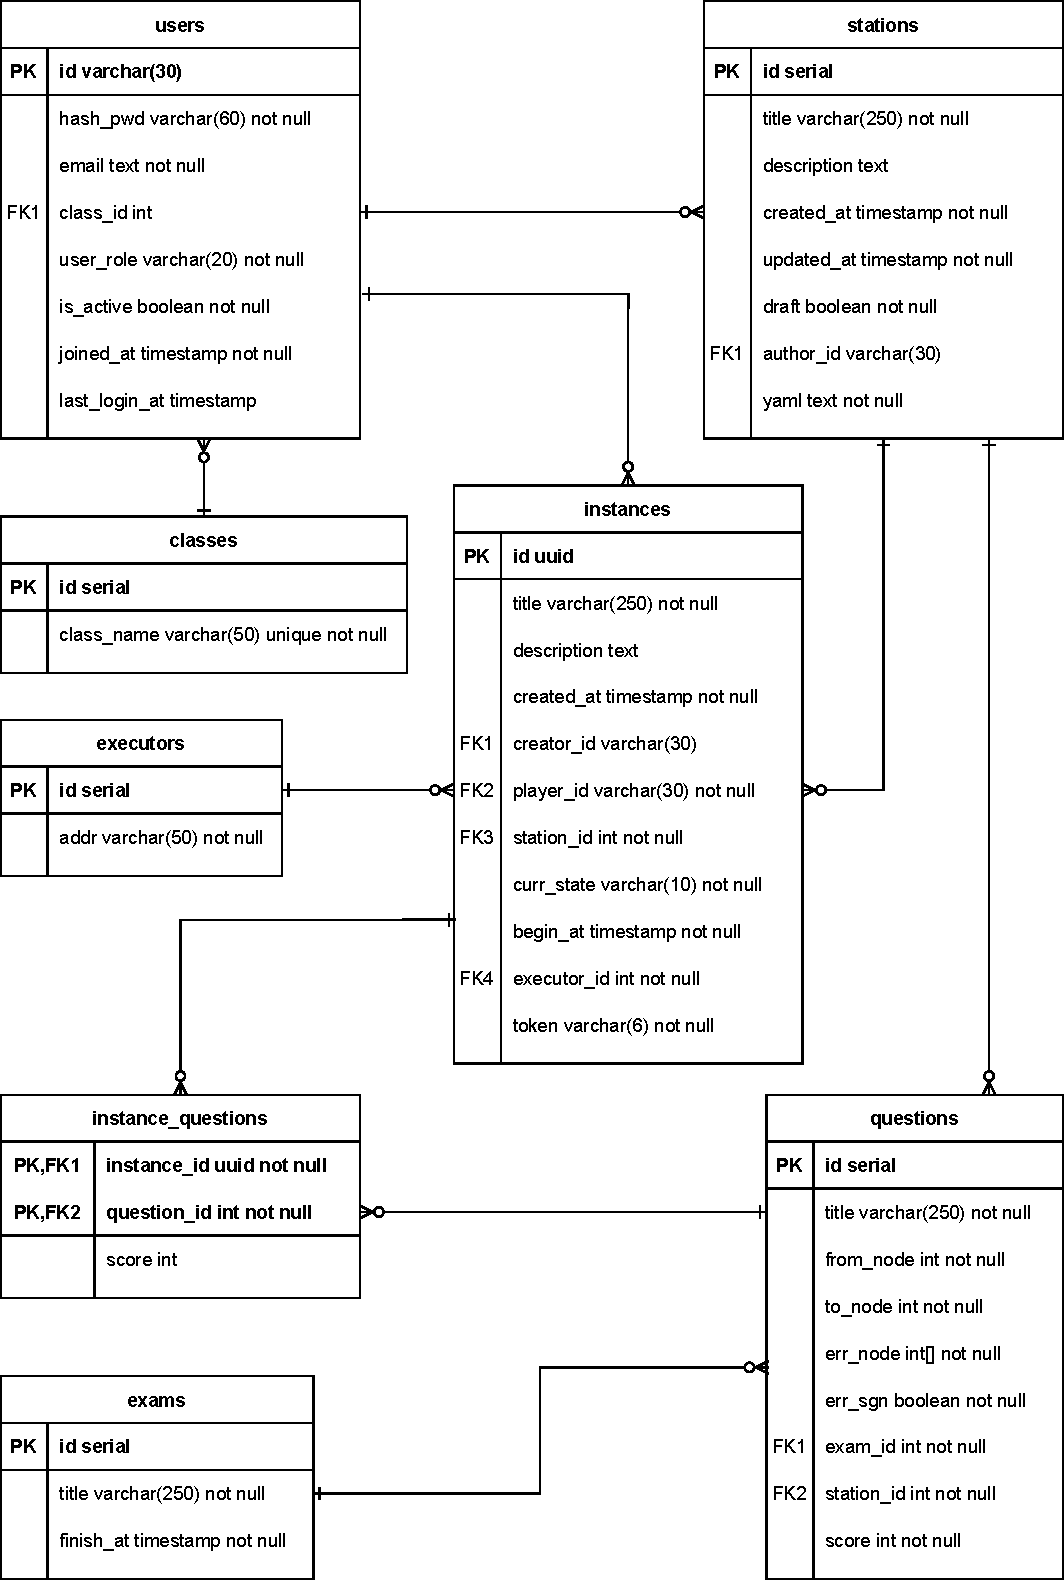
\includegraphics[width=0.95\textwidth]{figures/pdf/erd.pdf}
    \caption{\label{erd}数据库实体关系图}
\end{figure}

\subsubsection{表结构}

\paragraph 班级classes

\begin{lstlisting}
CREATE TABLE classes(
    id         serial       primary key,
    class_name varchar(50)  unique not null
)
\end{lstlisting}
主键id为自增整数,class\_name为班级名称

\paragraph 用户users

\begin{lstlisting}
CREATE TABLE users (
    id             varchar(30)     primary key,
    hash_pwd       varchar(60)     not null,
    email          text            not null,
    class_id       int  references classes(id) on delete set null,
    user_role      varchar(20)     not null,
    is_active      boolean         not null default 't',
    joined_at      timestamp       not null default now(),
    last_login_at  timestamp       default now()
)
\end{lstlisting}
解释:
\begin{itemize}
    \item 主键为id,类型为字符串,即用户自定义的用户id
    \item hash\_pwd 为加密后的用户密码
    \item email 为用户的电子邮箱地址
    \item class\_id 是表classes 的外键,表示用户所属的班级
    \item user\_role 表示用户角色
    \item is\_active 表示账户是否可用(未被禁用)
    \item joined\_at 和 last\_login\_at 默认是插入时的时间
\end{itemize}

\paragraph 车站stations

\begin{lstlisting}
CREATE TABLE stations (
    id          serial        primary key,
    title       varchar(250)  not null,
    description text,
    created_at  timestamp     not null default now(),
    updated_at  timestamp     not null default now(),
    draft       boolean       not null default 'f',
    author_id varchar(30) references users(id) on delete set null,
    yaml        text          not null
)
\end{lstlisting}
解释:
\begin{itemize}
    \item 主键为id, 自增整数
    \item title 为车站的标题
    \item description 为可空键,表示车站的备注
    \item draft 表示是否为草稿
    \item author\_id 是表 users 的外键,表示作者
    \item created\_at 和 updated\_at 默认是插入时的时间
    \item yaml 即为车站的描述文件内容
\end{itemize}

\paragraph 执行器executors

\begin{lstlisting}
CREATE TABLE executors (
    id             serial        primary key,
    addr           varchar(50)   not null
)
\end{lstlisting}
addr是该runtime的地址。

\paragraph 考试exams

\begin{lstlisting}
CREATE TABLE exams (
    id           serial        primary key,
    title        varchar(250)  not null,
    finish_at    timestamp     not null
)
\end{lstlisting}
finish\_at 表示结束时间,是考试特有的属性。

\paragraph 实例instances

\begin{lstlisting}
CREATE TABLE instances (
    id      uuid    primary key default gen_random_uuid(),
    title   varchar(250)  not null,
    description text,
    created_at  timestamp     not null  default now(),
    creator_id  varchar(30) references users(id) on delete ...,
    player_id   varchar(30)   not null  references users(id),    
    station_id  int           not null  references stations(id),
    curr_state  varchar(10)   not null,
    begin_at    timestamp     not null  default now(),
    executor_id int           not null  references executors(id),
    token       varchar(6)    not null
)
\end{lstlisting}
解释:
\begin{itemize}
    \item 主键为id, 类型是uuid
    \item title 为实例标题
    \item curr\_state 表示实例当前的状态
    \item creator\_id 是表 users 的外键,表示创建者
    \item player\_id 是表 users 的外键,表示实例的用户
    \item created\_at  默认是插入时的时间
    \item begin\_at 表示实例的开始时间
    \item executor\_id 表示该实例的运行时id,是executors表的外键
    \item station\_id 是表 stations 的外键,表示实例的车站
    \item token 是游客令牌
\end{itemize}

\paragraph 问题questions

\begin{lstlisting}
CREATE TABLE questions (
    id          serial        primary key,
    title       varchar(250)  not null,
    from_node   int           not null,
    to_node     int           not null,
    err_node    int[]         not null,
    err_sgn     boolean       not null,
    exam_id     int           not null  references exams(id),
    station_id  int           not null  references stations(id),
    score       int           not null
)
\end{lstlisting}
解释:
\begin{itemize}
    \item from\_node 是本题目进路自何处
    \item to\_node 是本题目进路往何处
    \item err\_node 是本题目的预设故障结点
    \item err\_dgn 是本题目进路信号机是否出错
    \item exam\_id 是表 exams 的外键,表示本题目属于哪个考试
    \item station\_id 是表 stations 的外键,表示本题目属于哪个车站
    \item score 表示本道题赋分几何
\end{itemize}

\paragraph 实例问题(即“考题”)instance\_questions

\begin{lstlisting}
CREATE TABLE instance_questions (
    instance_id    uuid   not null references instances(id),
    question_id    int    not null references questions(id),
    score          int,
    PRIMARY KEY (instance_id, question_id)
)
\end{lstlisting}

本表使用instance\_id和question\_id两个外键作为联合主键,本表的一个记录表示
某个实例(必然为考试实例)的某个题目得分几何。score是可空的,因为在新建考试实例的
时候就会在本表中新建进路,在完成某道考题的时候更新记录。

\subsection{持久层}
\subsubsection{ORM}
本案采用ORM以提升开发效率,ORM 是一种程序设计技术,用于将数据库的记录映射到程序语言的对象中,
或者将对象映射到某个表中,其封装了CRUD的SQL语句操作,可以让开发者从表中直接读入一个对象。或者将
一个对象插入某个表。效果上说,它其实是创建了一个可在编程语言里使用的“虚拟对象数据库”。

在本案的持久层 uroj-db 中,定义了程序的DAO层逻辑,封装了所有项目需要的数据库访问方法。
以便供Api, Auth, Executor 等服务复用。uroj采用diesel作为本案的ORM库,
将DAO层的各种结构体定义和上小结所定义的SQL表映射起来的,
就是diesel client所生成的schema。

这里简单介绍一下 diesel 的使用步骤。首先需要定义migration,migration可以简单理解为创建和删除表
的sql文件。将上一节的表定义好后。使用diesel生成schema,schema是diesel使用
rust macro定义的一些字段。之后我们需要定义DAO层的struct,对于一个表一般而言需要两种
struct,一个是读取用一个是插入用,但需要derive diesel提供的相应的过程宏,这样就可以
将sql表和DAO 层 struct映射起来,再使用diesel提供的方法进行CRUD操作。

\subsubsection{连接池}
连接池(英语:connection pool)是维护的数据库连接的缓存,
以便在将来需要对数据库发出请求时可以重用连接。
每次需要再打开一个新的数据库连接都是低效的,而且在高流量条件下会导致资源耗尽。
可以使用连接池解决这个问题以提高在数据库上执行命令的性能。
为每个用户打开和维护数据库连接,尤其是对动态数据库驱动的网站应用程序发出的请求,
既昂贵又浪费资源。在连接池中,创建连接之后,将连接放在池中并再次使用,这样就不必创建新的连接。
如果所有连接都正在使用,则创建一个新连接并将其添加到池中。
连接池还减少了用户必须等待创建与数据库的连接的时间。

uroj 采用 r2d2 作为数据库连接池,r2d2 是rust的一个通用连接池。
r2d2对于它所管理的连接类型是不可知的。
ManageConnection特性的实现者提供了数据库特定的逻辑来创建和检查连接的健康状况。

在 uroj-db crate 中使用如下create\_connection\_pool函数创建一个连接池。在
uroj-api 和 uroj-runtime 使用本函数创建连接池。
\begin{lstlisting}
use diesel::r2d2::{ConnectionManager, Pool};
use diesel::{pg::PgConnection, r2d2::PooledConnection};

pub type PgPool = Pool<ConnectionManager<PgConnection>>;
pub type Conn = PooledConnection<ConnectionManager<PgConnection>>;

pub fn create_connection_pool() -> PgPool {
    let url = env::var("DATABASE_URL").expect("Can't get DB URL");
    let manager = ConnectionManager::<PgConnection>::new(url);
    Pool::builder()
        .build(manager)
        .expect("Failed to create pool")
}
\end{lstlisting}

\subsubsection{时区处理}
本项目从数据库PostgreSQL、业务逻辑层到前端的表现层,一个需要重视的问题是时区。
若是单时区应用的话大可以直接在数据库中保存北京时间的字符串,但本案为了保证通用性
,考虑来自不同时区的用户,或者是部署于不同时区的数据库、服务器。因此在PostgreSQL中,
本例使用时间戳(timestamp)保存时间,时间戳是UTC1970年1月1日0时0分0秒起至现在的总秒数。
因此是一种没有时区的信息,或者说是协调世界时0时区的时间。

从数据库中取到的时间戳,在业务逻辑层中被表示为 chrono 库中的 NaiveDateTime,NaiveDateTime是
一种没有时区的日期时间字面量,其可以被简单地转换成任何时区的DateTime,因此我们会在
业务逻辑层中将0时区的时间戳转换成业务逻辑层服务器所在时区的时间,并呈递给表现层。表现层
显示哪种时区完全取决于其访问部署于何处的服务器。

\clearpage
\section{测试}
\subsection{业务逻辑层服务}
业务逻辑层服务众多,如第四章介绍的,但测试流程基本上相同,这里只拿典型举例:
\subsubsection{获取车站布局测试}
测试输入(其中的实例id是之前创建的):
\begin{lstlisting}
query {
  stationLayout(id: "db42f0ed-d096-4805-b048-909e69dd44e2") {
    title,
    nodes{
      nodeId, 
      trackId, 
      leftP{x,y}, 
      rightP{x,y}, 
      leftJoint, 
      rightJoint
    },
    signals{
      signalId,
      sgnType,
      sgnMnt,
      protectNodeId,
      side,
      dir,
      pos{x,y},
      btns
    }
  }
}
\end{lstlisting}

服务输出:
\begin{lstlisting}
{
  "data": {
    "stationLayout": {
      "nodes": [
        {
          "leftJoint": "EMPTY",
          "leftP": {
            "x": 0,
            "y": 5
          },
          "nodeId": 1,
          "rightJoint": "NORMAL",
          "rightP": {
            "x": 5,
            "y": 5
          },
          "trackId": "X3JG"
        },
        {
          "leftJoint": "NORMAL",
          "leftP": {
            "x": 5,
            "y": 5
          },
          "nodeId": 5,
          "rightJoint": "NORMAL",
          "rightP": {
            "x": 5,
            "y": 10
          },
          "trackId": "IAG"
        }
      ],
      "signals": [
        {
          "btns": [
            "PASS",
            "GUIDE",
            "TRAIN"
          ],
          "dir": "LEFT",
          "pos": {
            "x": 5,
            "y": 5
          },
          "protectNodeId": 5,
          "sgnMnt": "POST_MOUNTING",
          "sgnType": "HOME_SIGNAL",
          "side": "UPPER",
          "signalId": "X"
        }
      ],
      "title": "测试站"
    }
  }
}
\end{lstlisting}
\subsection{控制台界面}
\begin{figure}[htbp!]
  \centering
  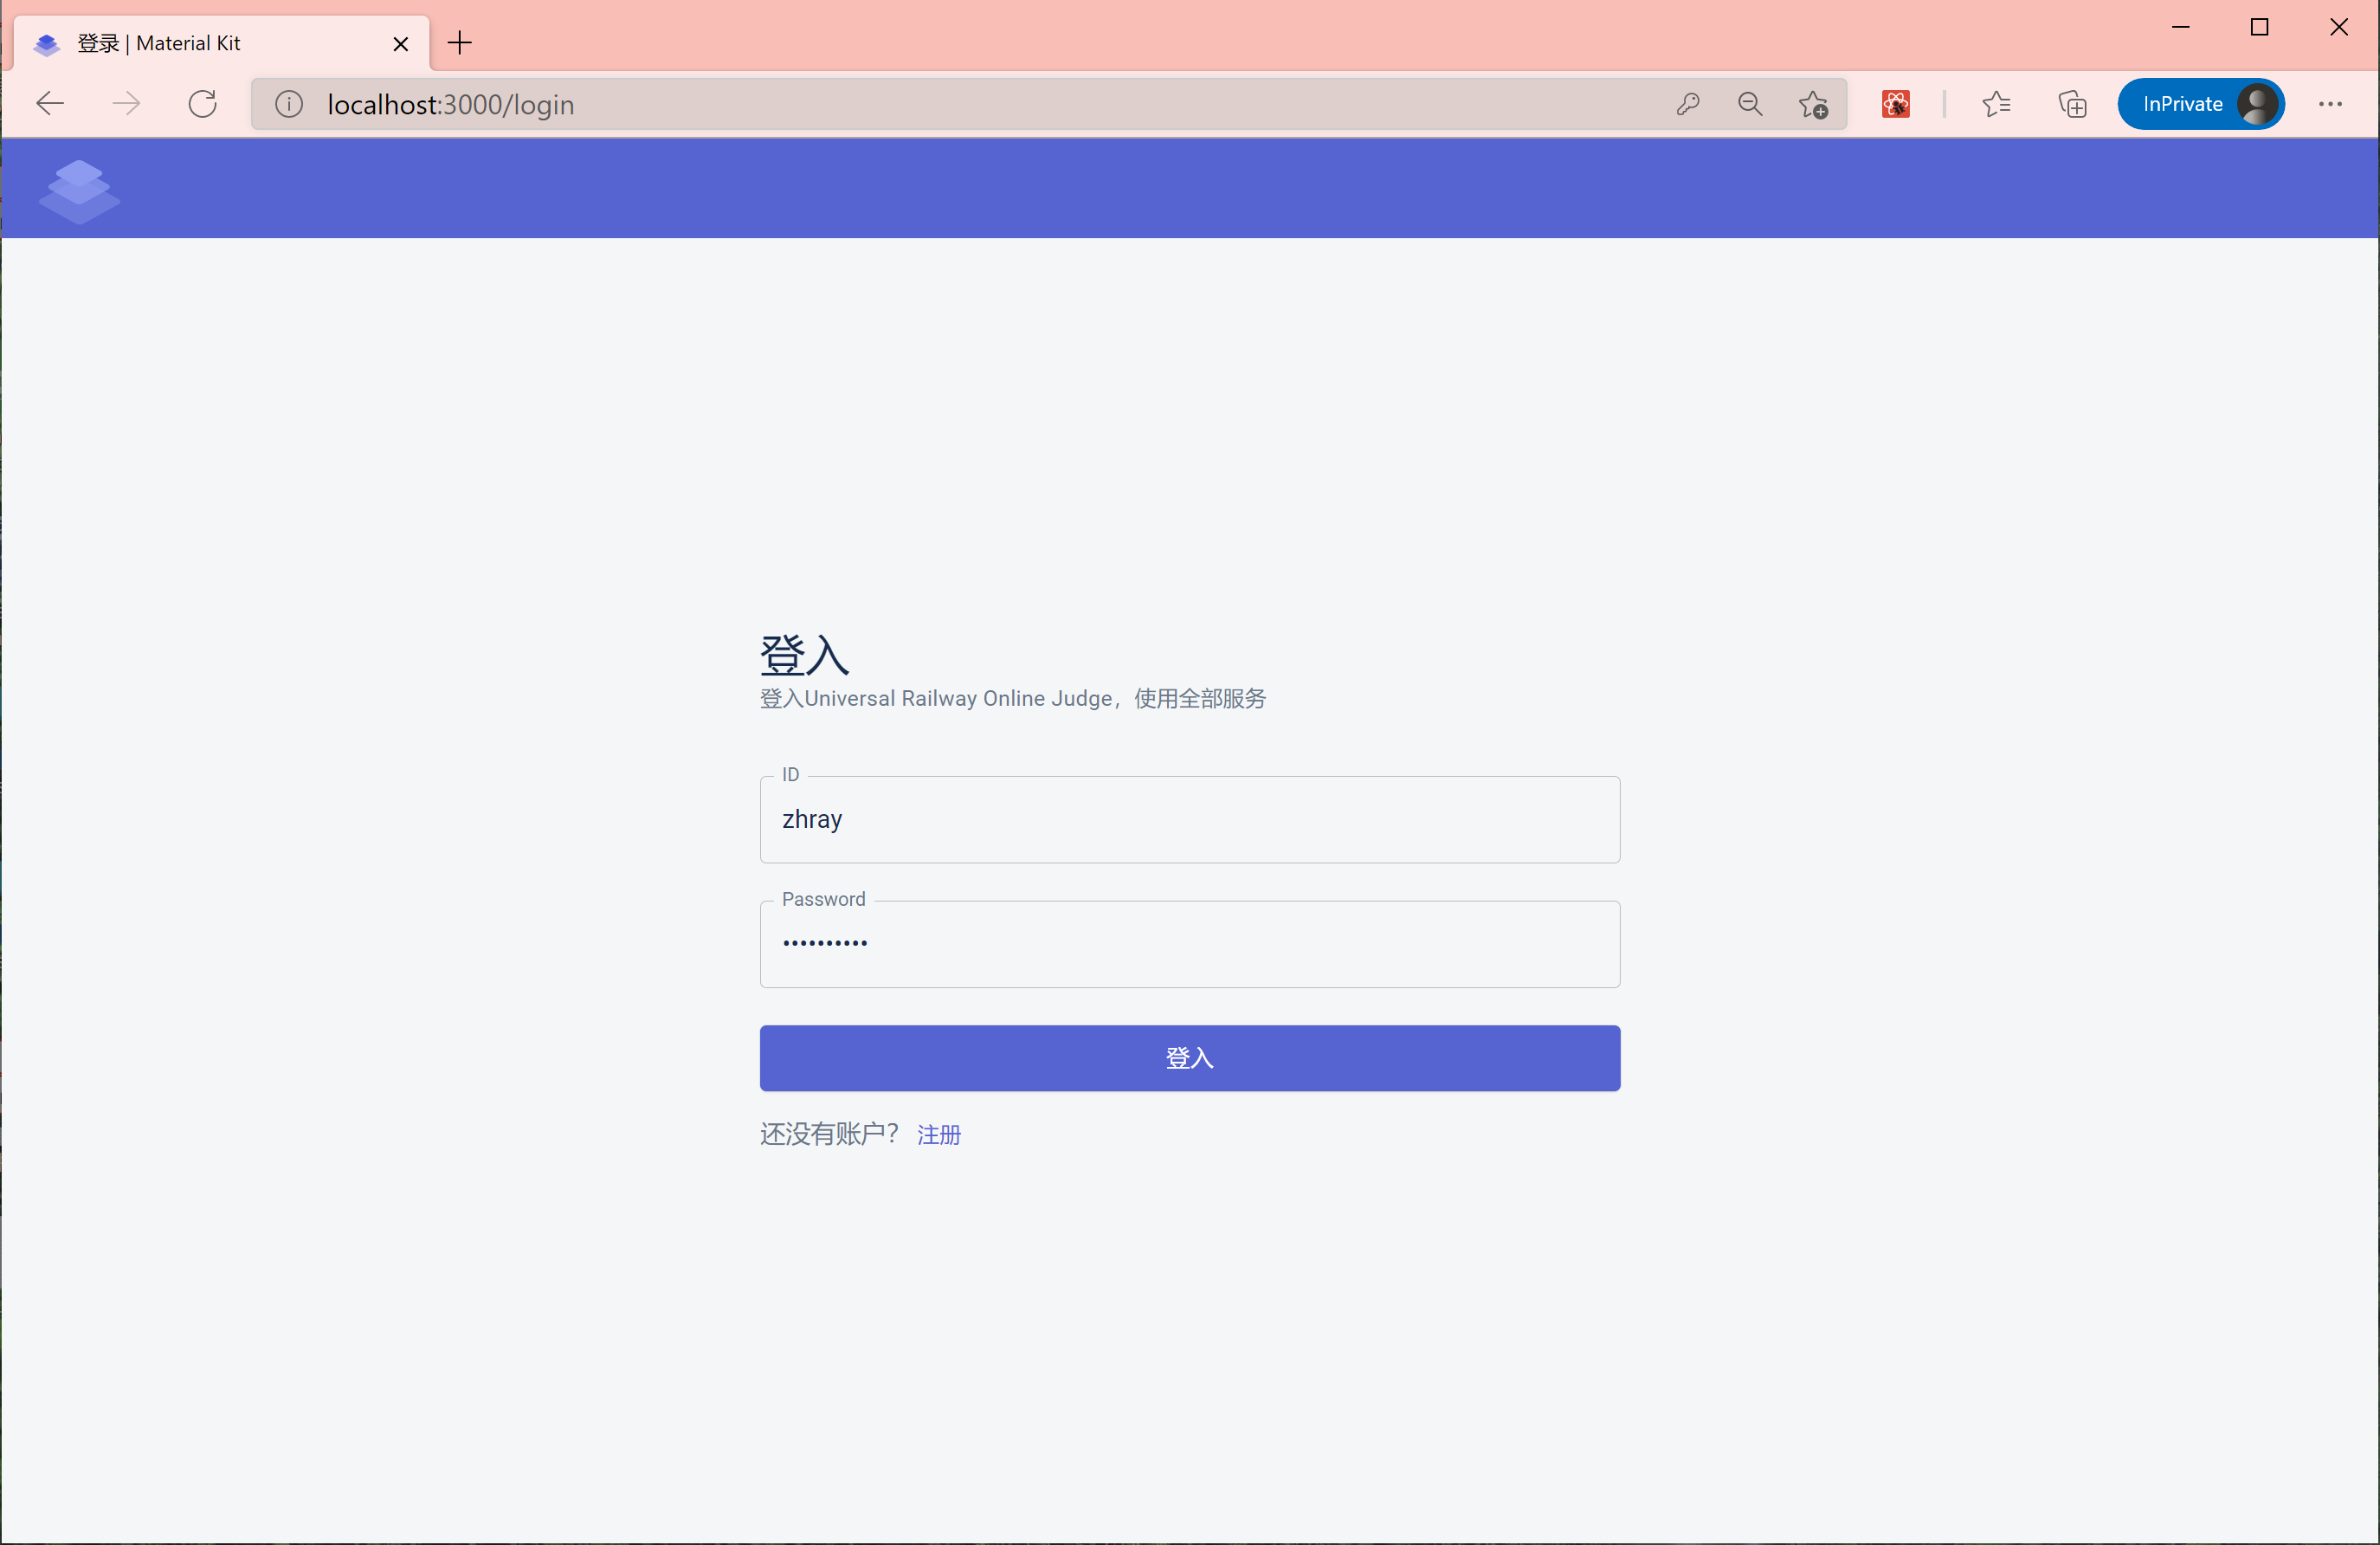
\includegraphics[width=\textwidth]{figures/png/login.png}
  \caption{\label{login}登录界面}
\end{figure}

登录界面如图\ref{login} 所示,当登录成功后,系统会跳转页面至控制台。
如果登陆失败则会报错

\begin{figure}[htbp!]
  \centering
  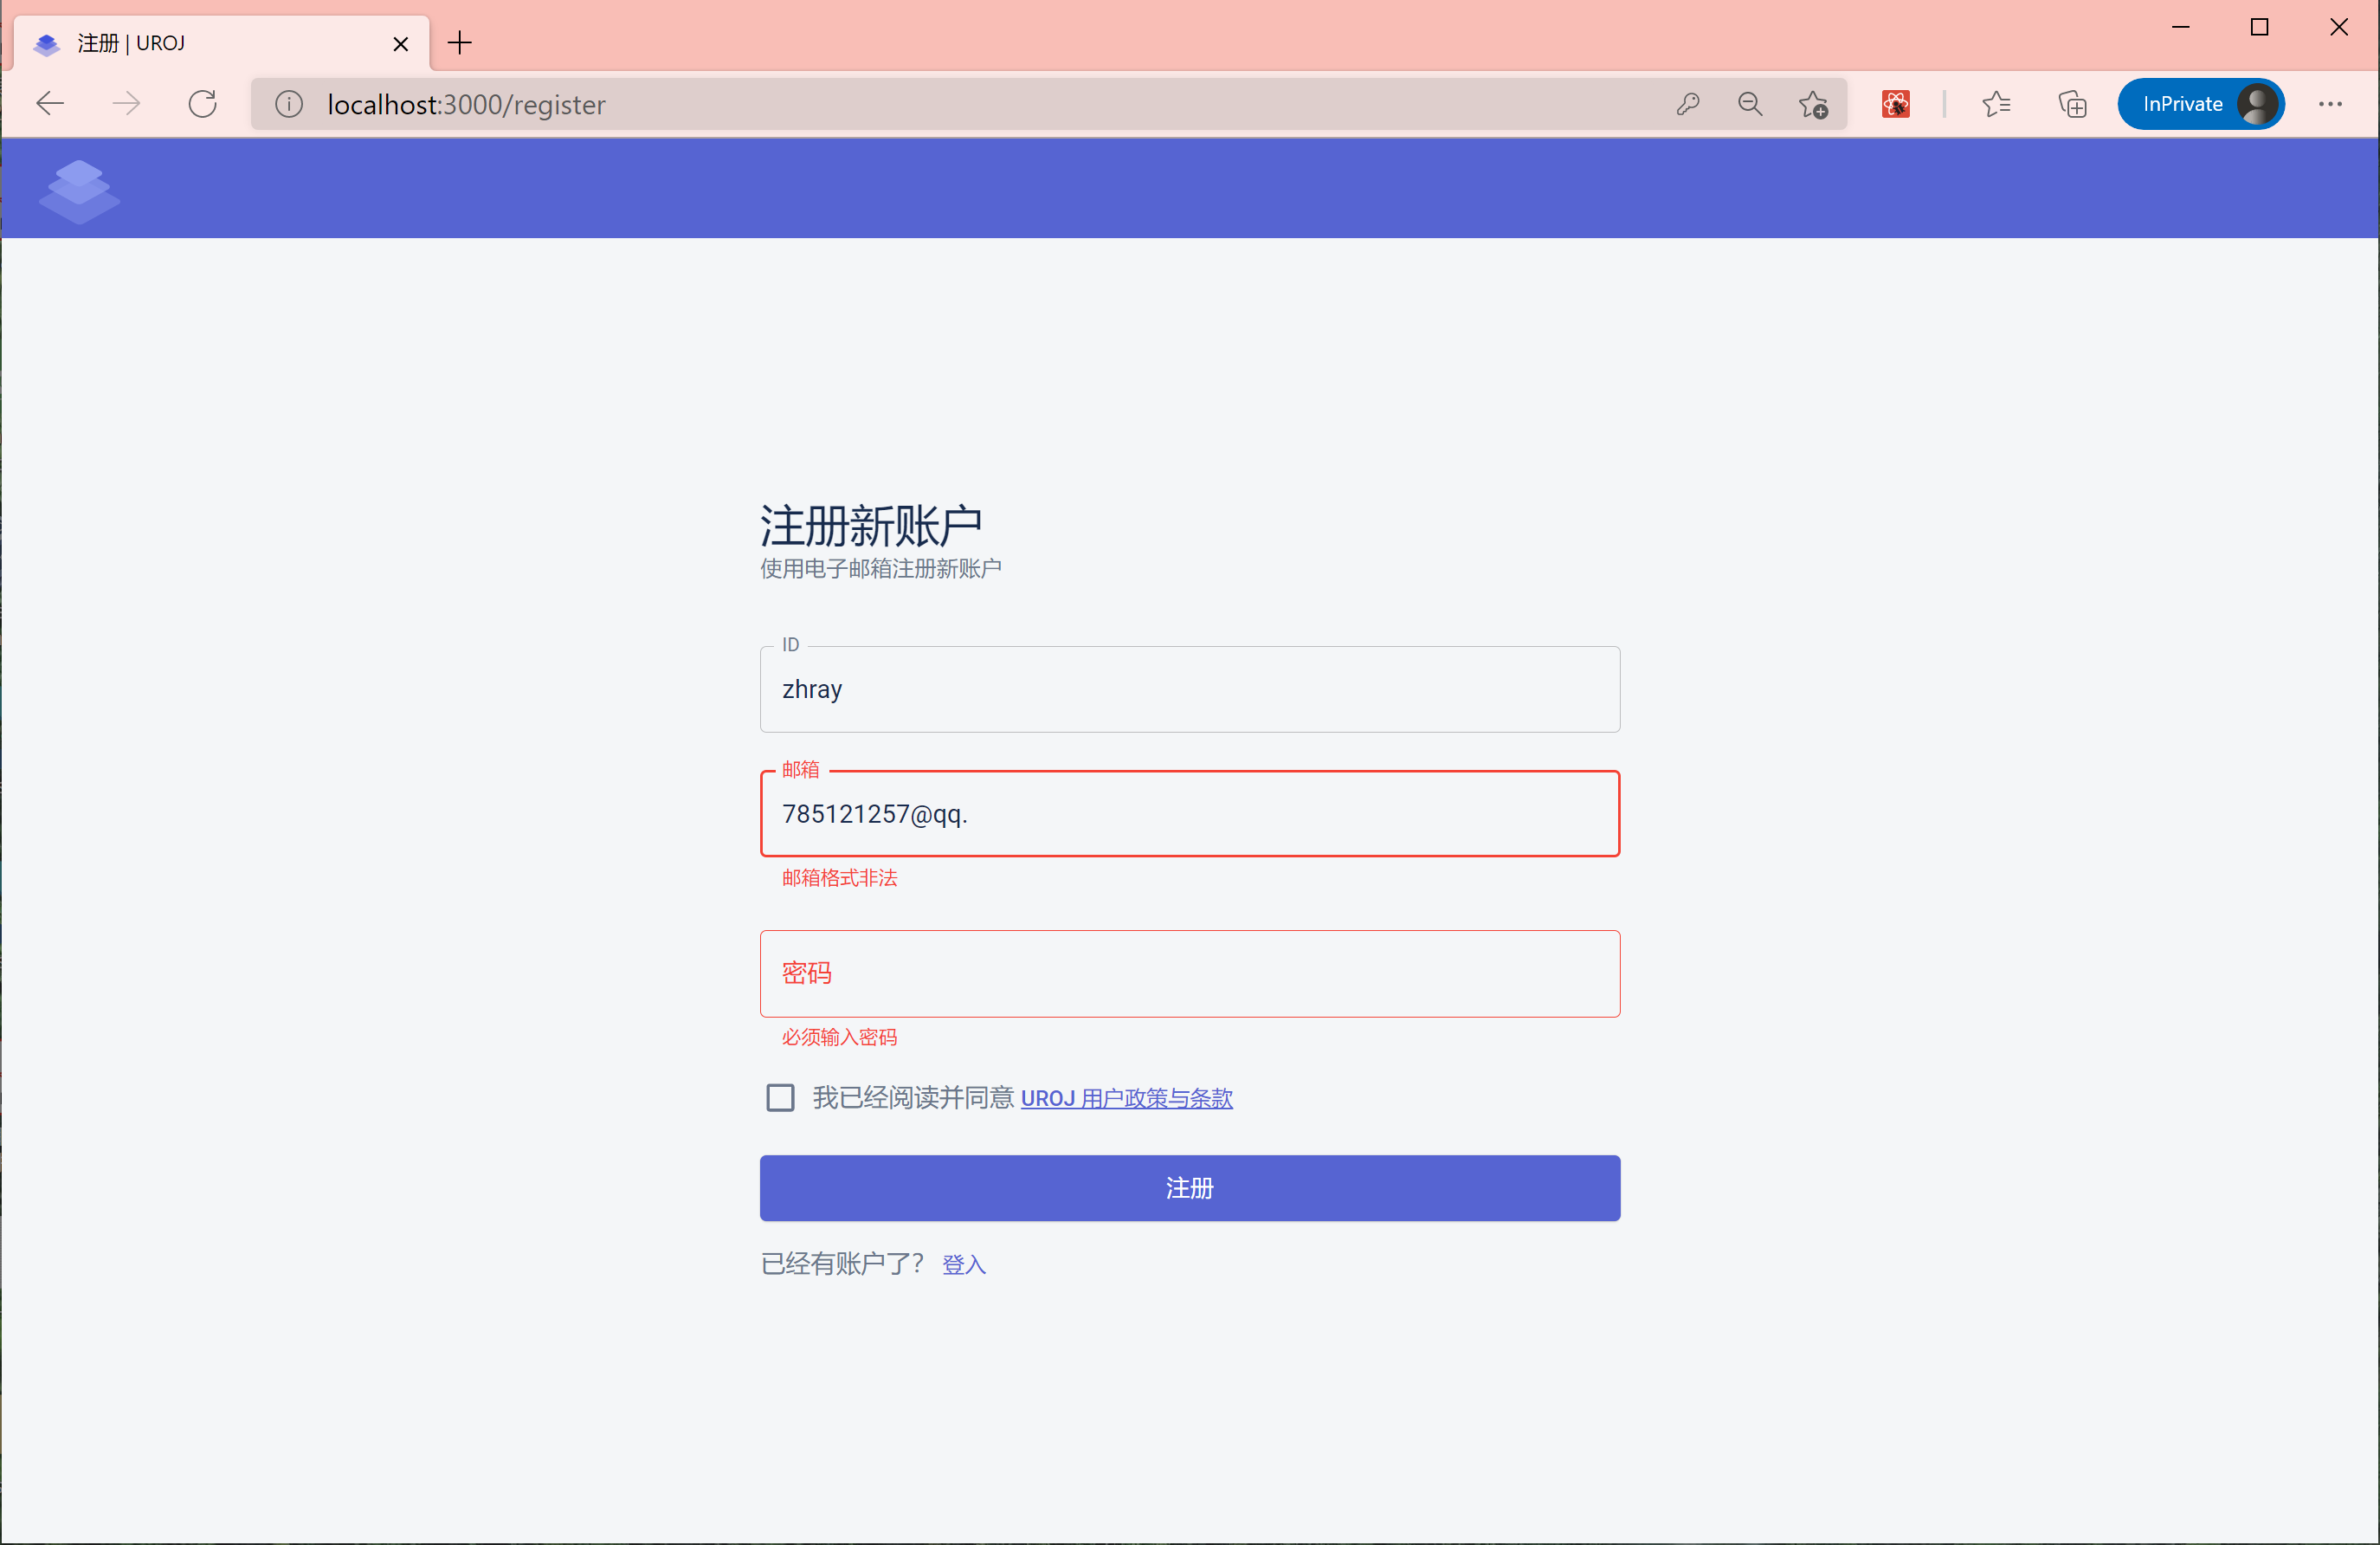
\includegraphics[width=\textwidth]{figures/png/input_err.png}
  \caption{\label{input_err}注册}
\end{figure}

注册界面如图\ref{input_err} 所示,当注册成功后,系统会询问是否跳转页面至登录。
如果注册失败则会报错

\begin{figure}[htbp!]
  \centering
  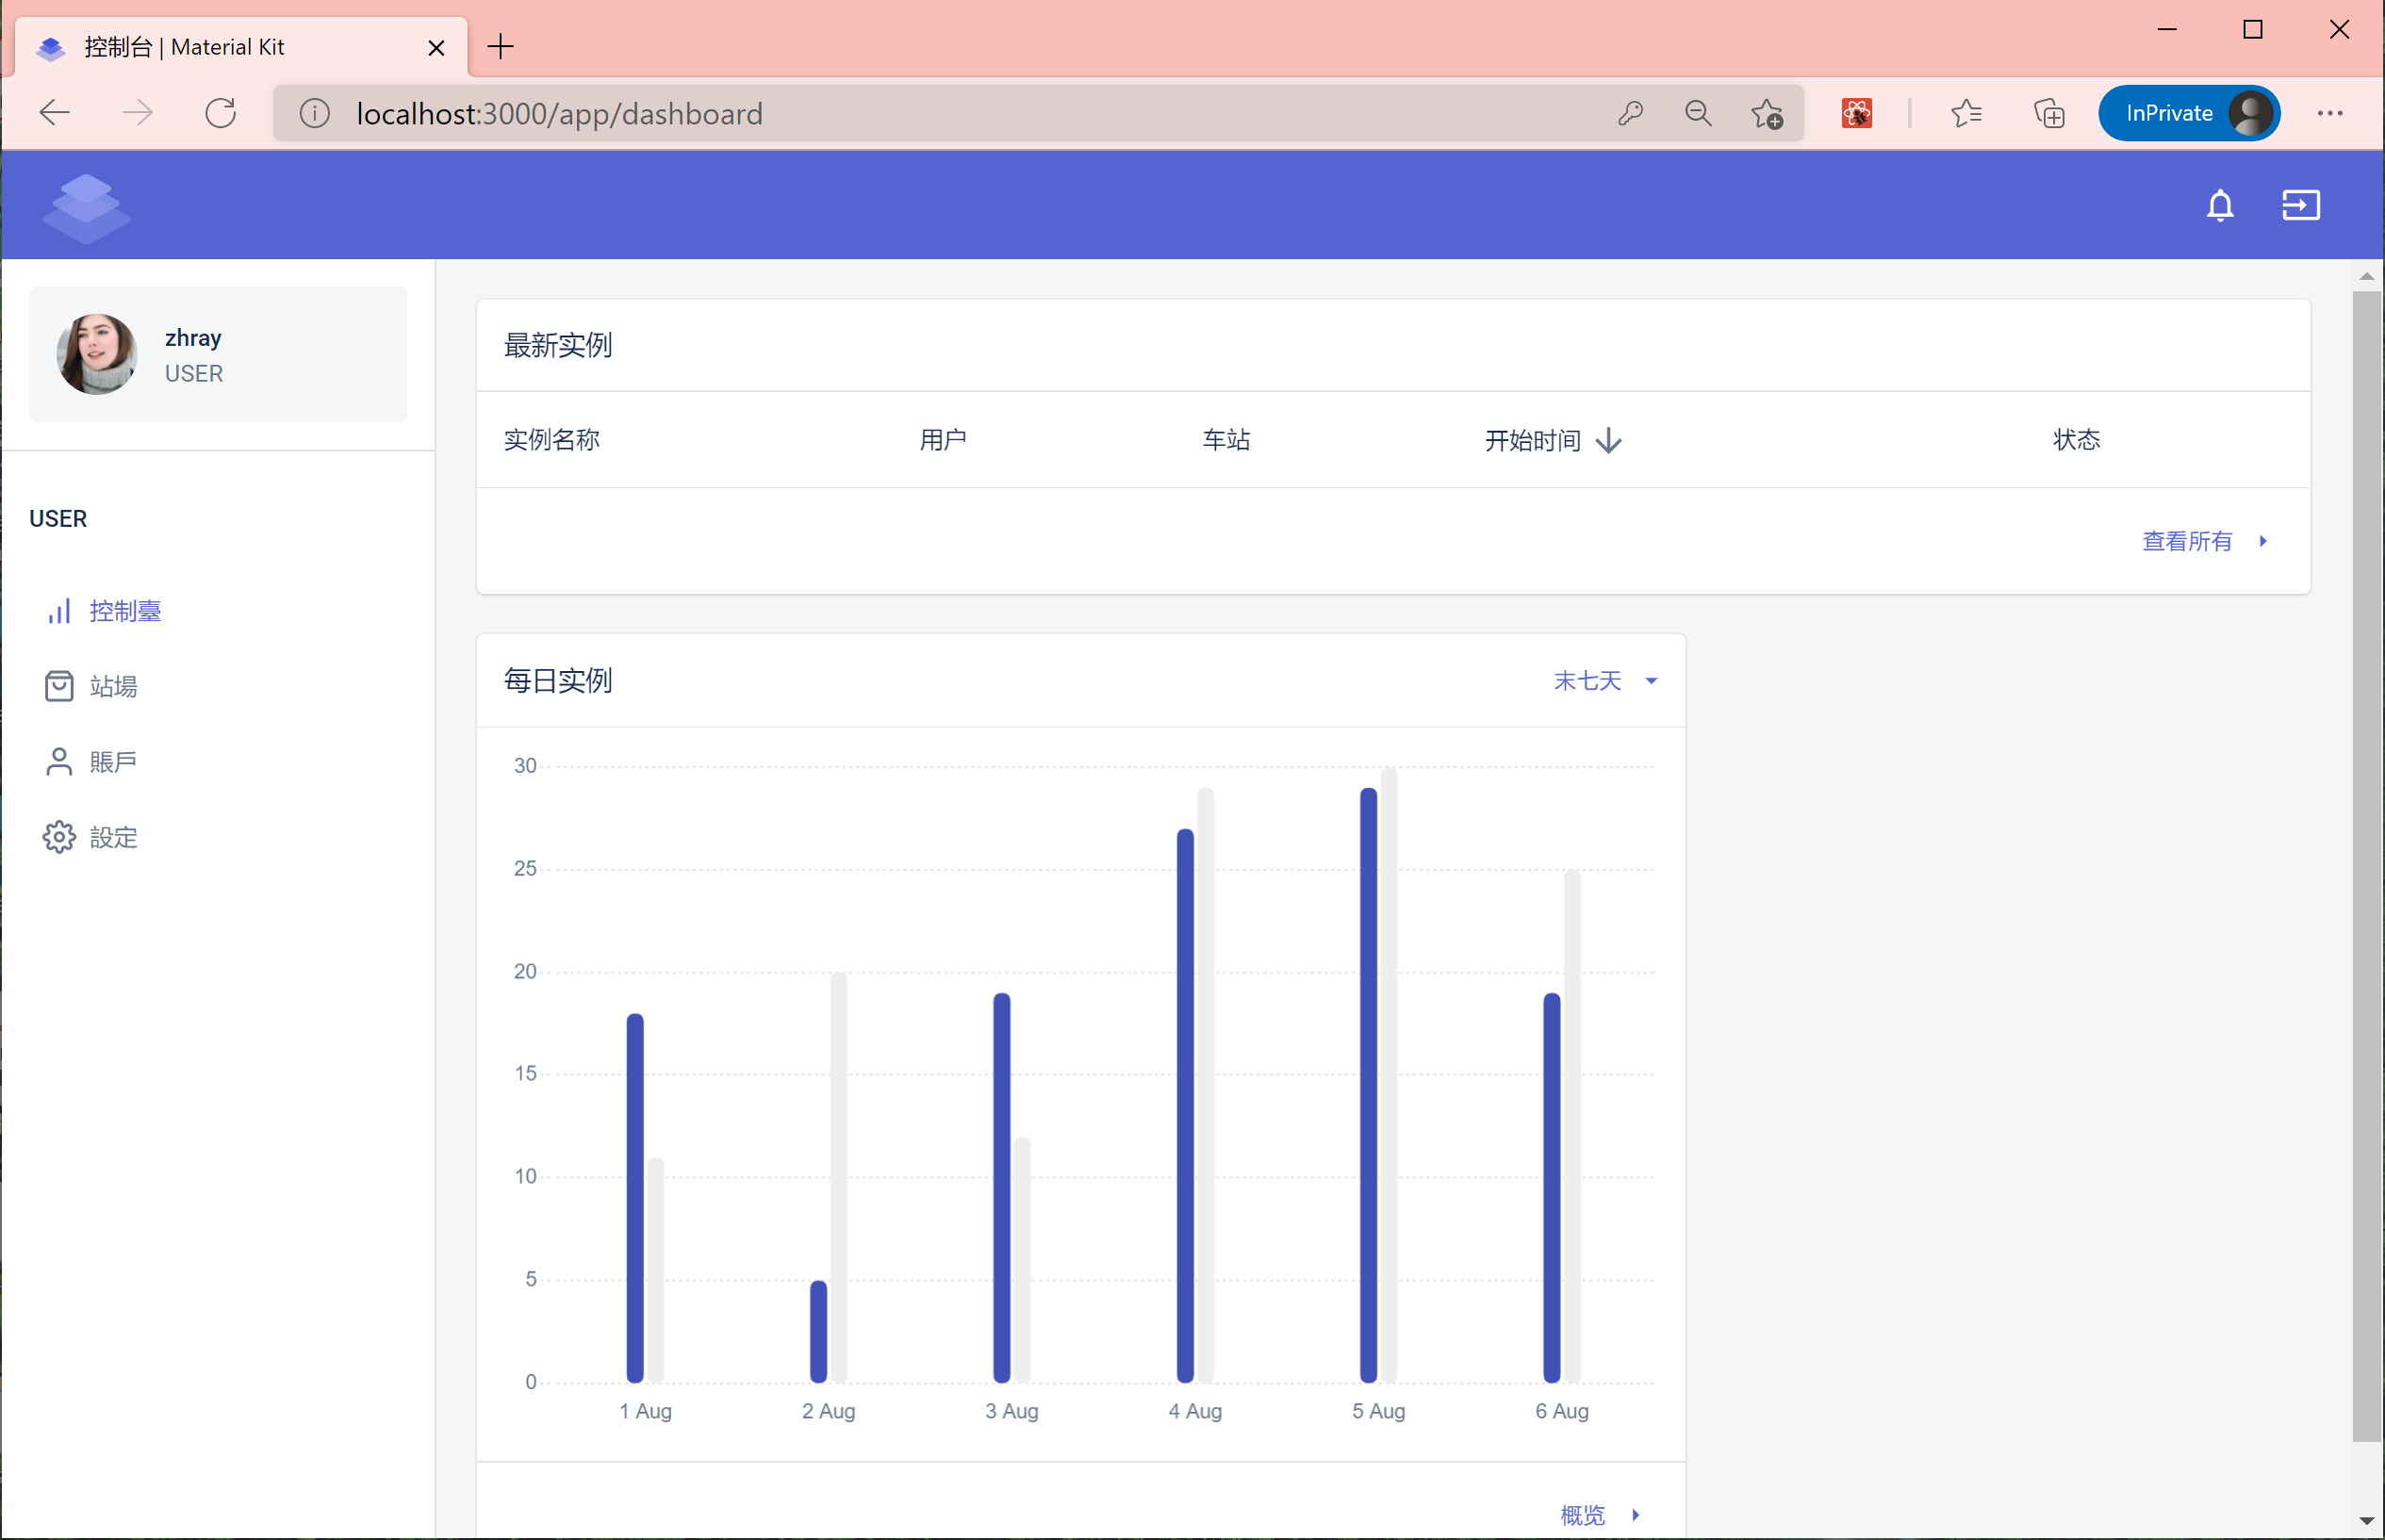
\includegraphics[width=\textwidth]{figures/png/user_ui.png}
  \caption{\label{user_ui}用户角色的控制台首页}
\end{figure}

USER 角色的控制台界面如图\ref{user_ui} 所示,在侧边栏中是可供用户
点入的功能清单。

\begin{figure}[htbp!]
  \centering
  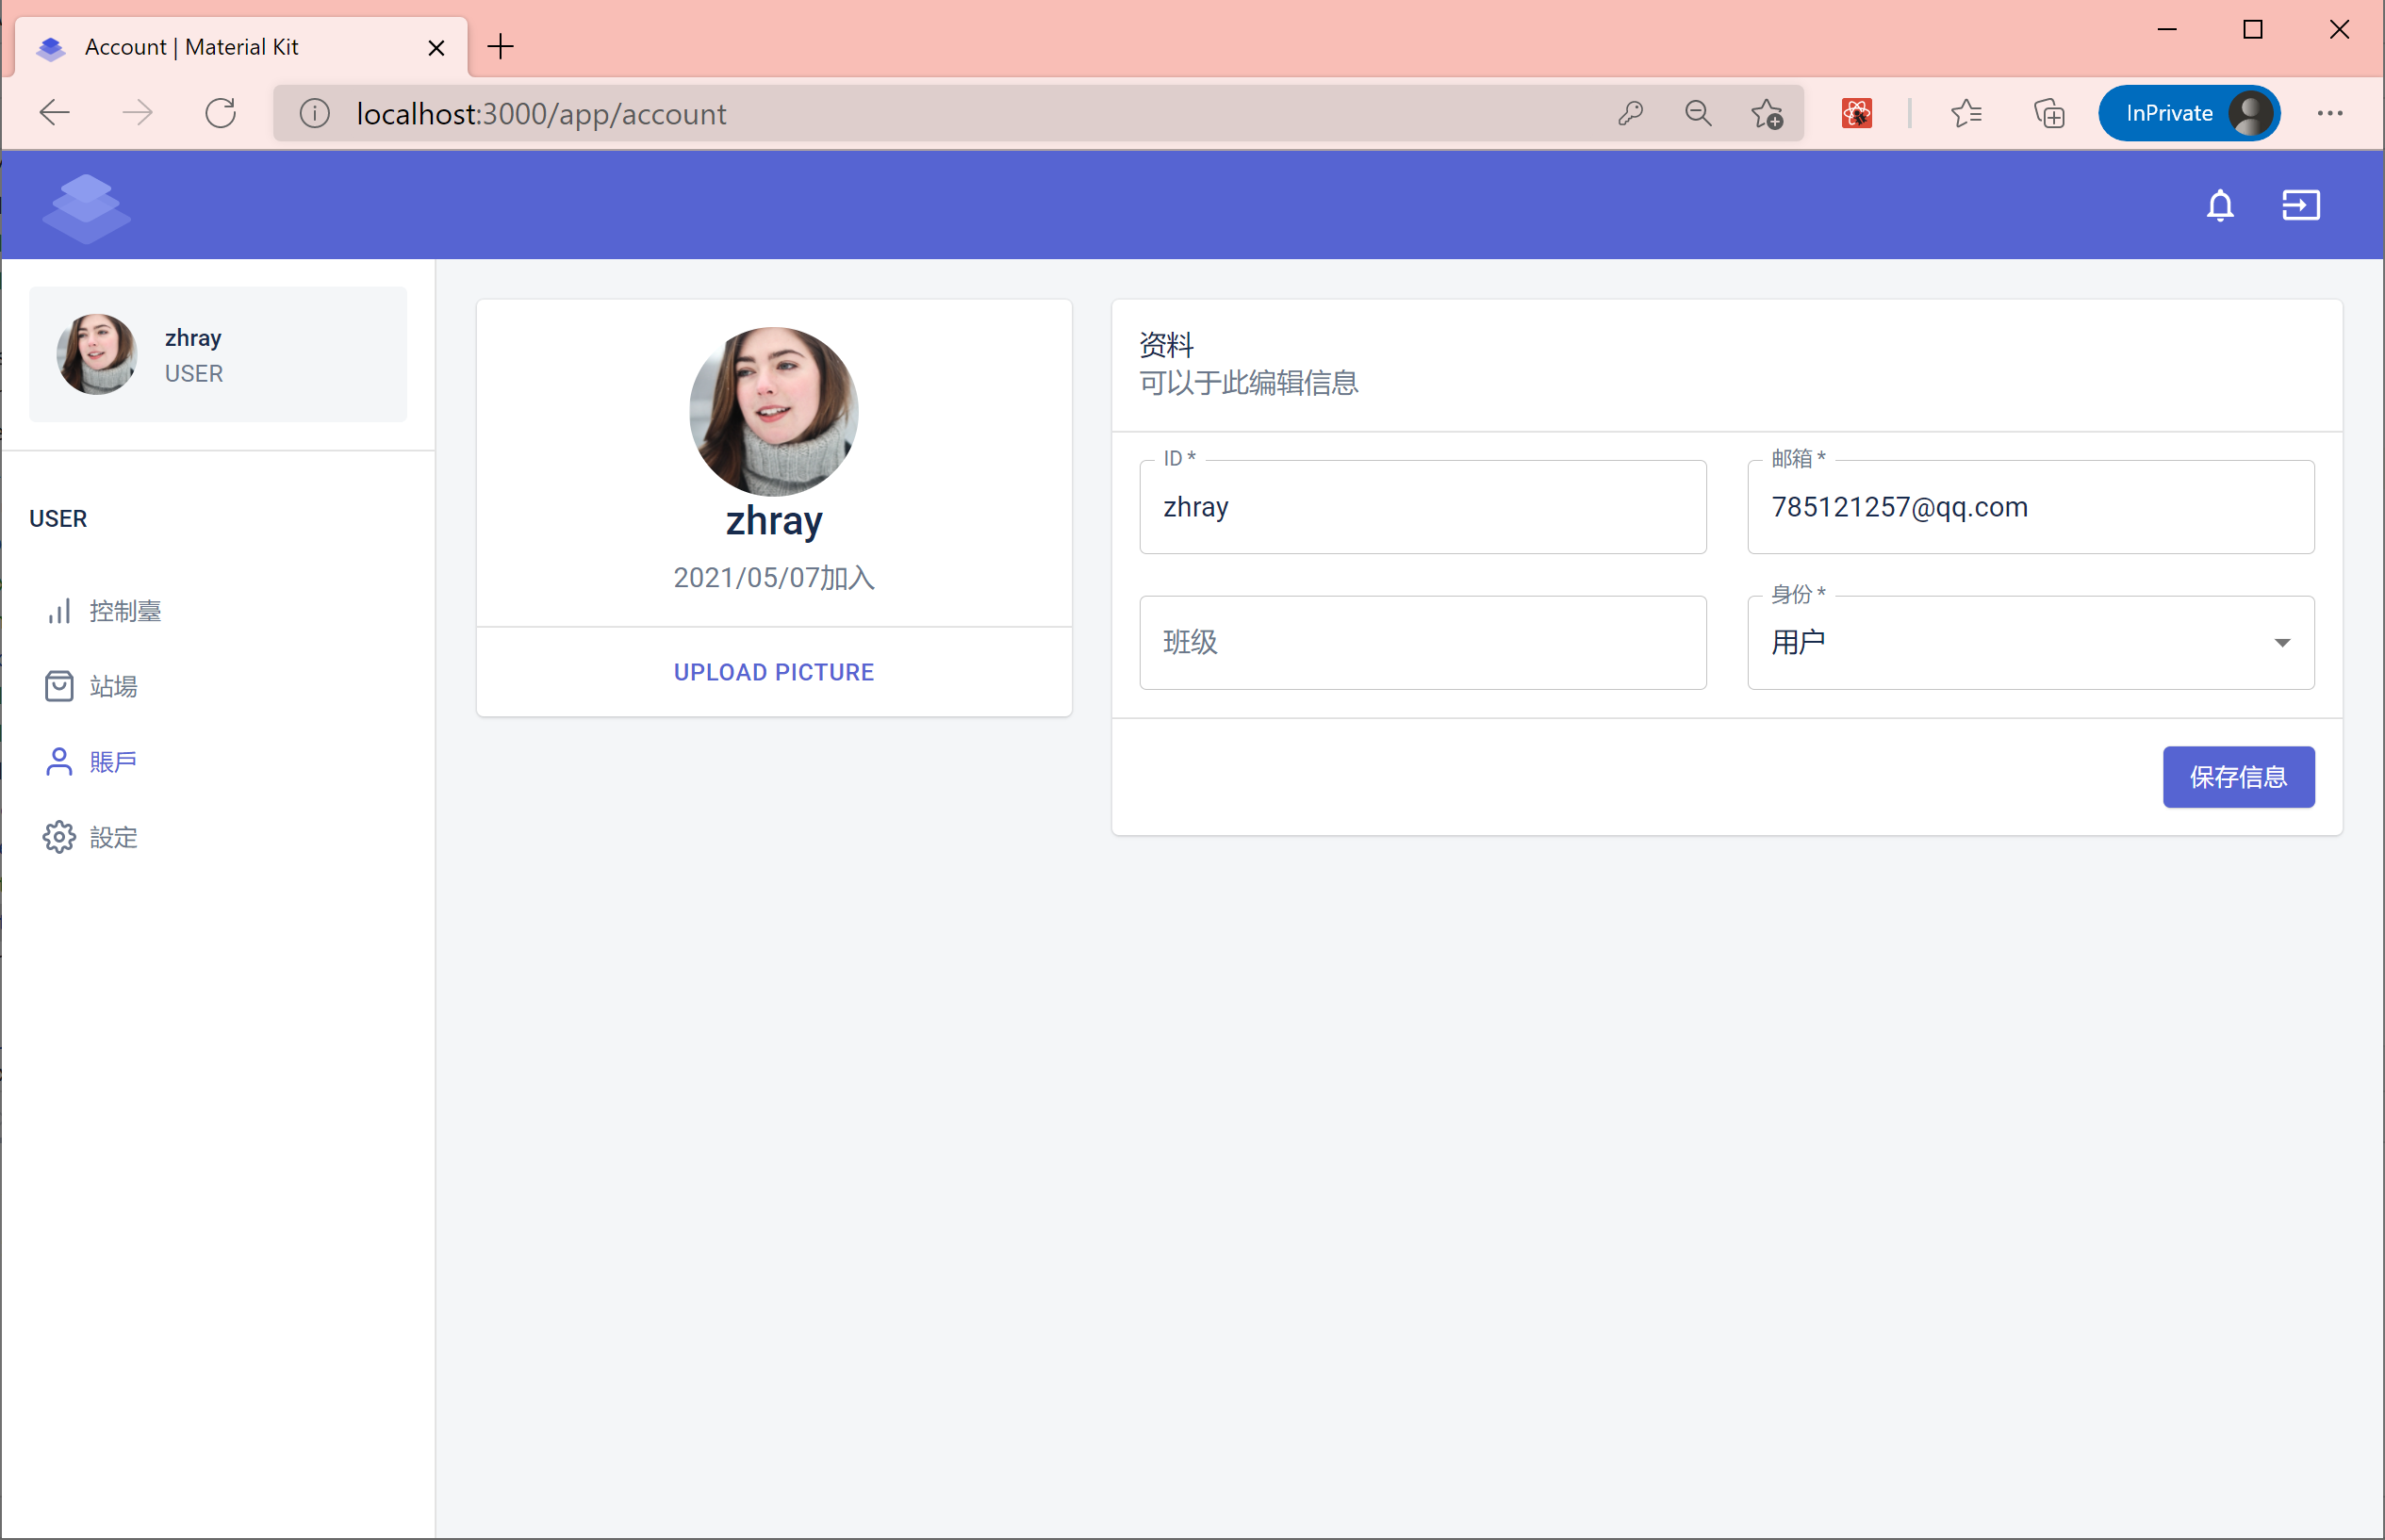
\includegraphics[width=\textwidth]{figures/png/user_data.png}
  \caption{\label{user_data}用户信息页}
\end{figure}

\begin{figure}[htbp!]
  \centering
  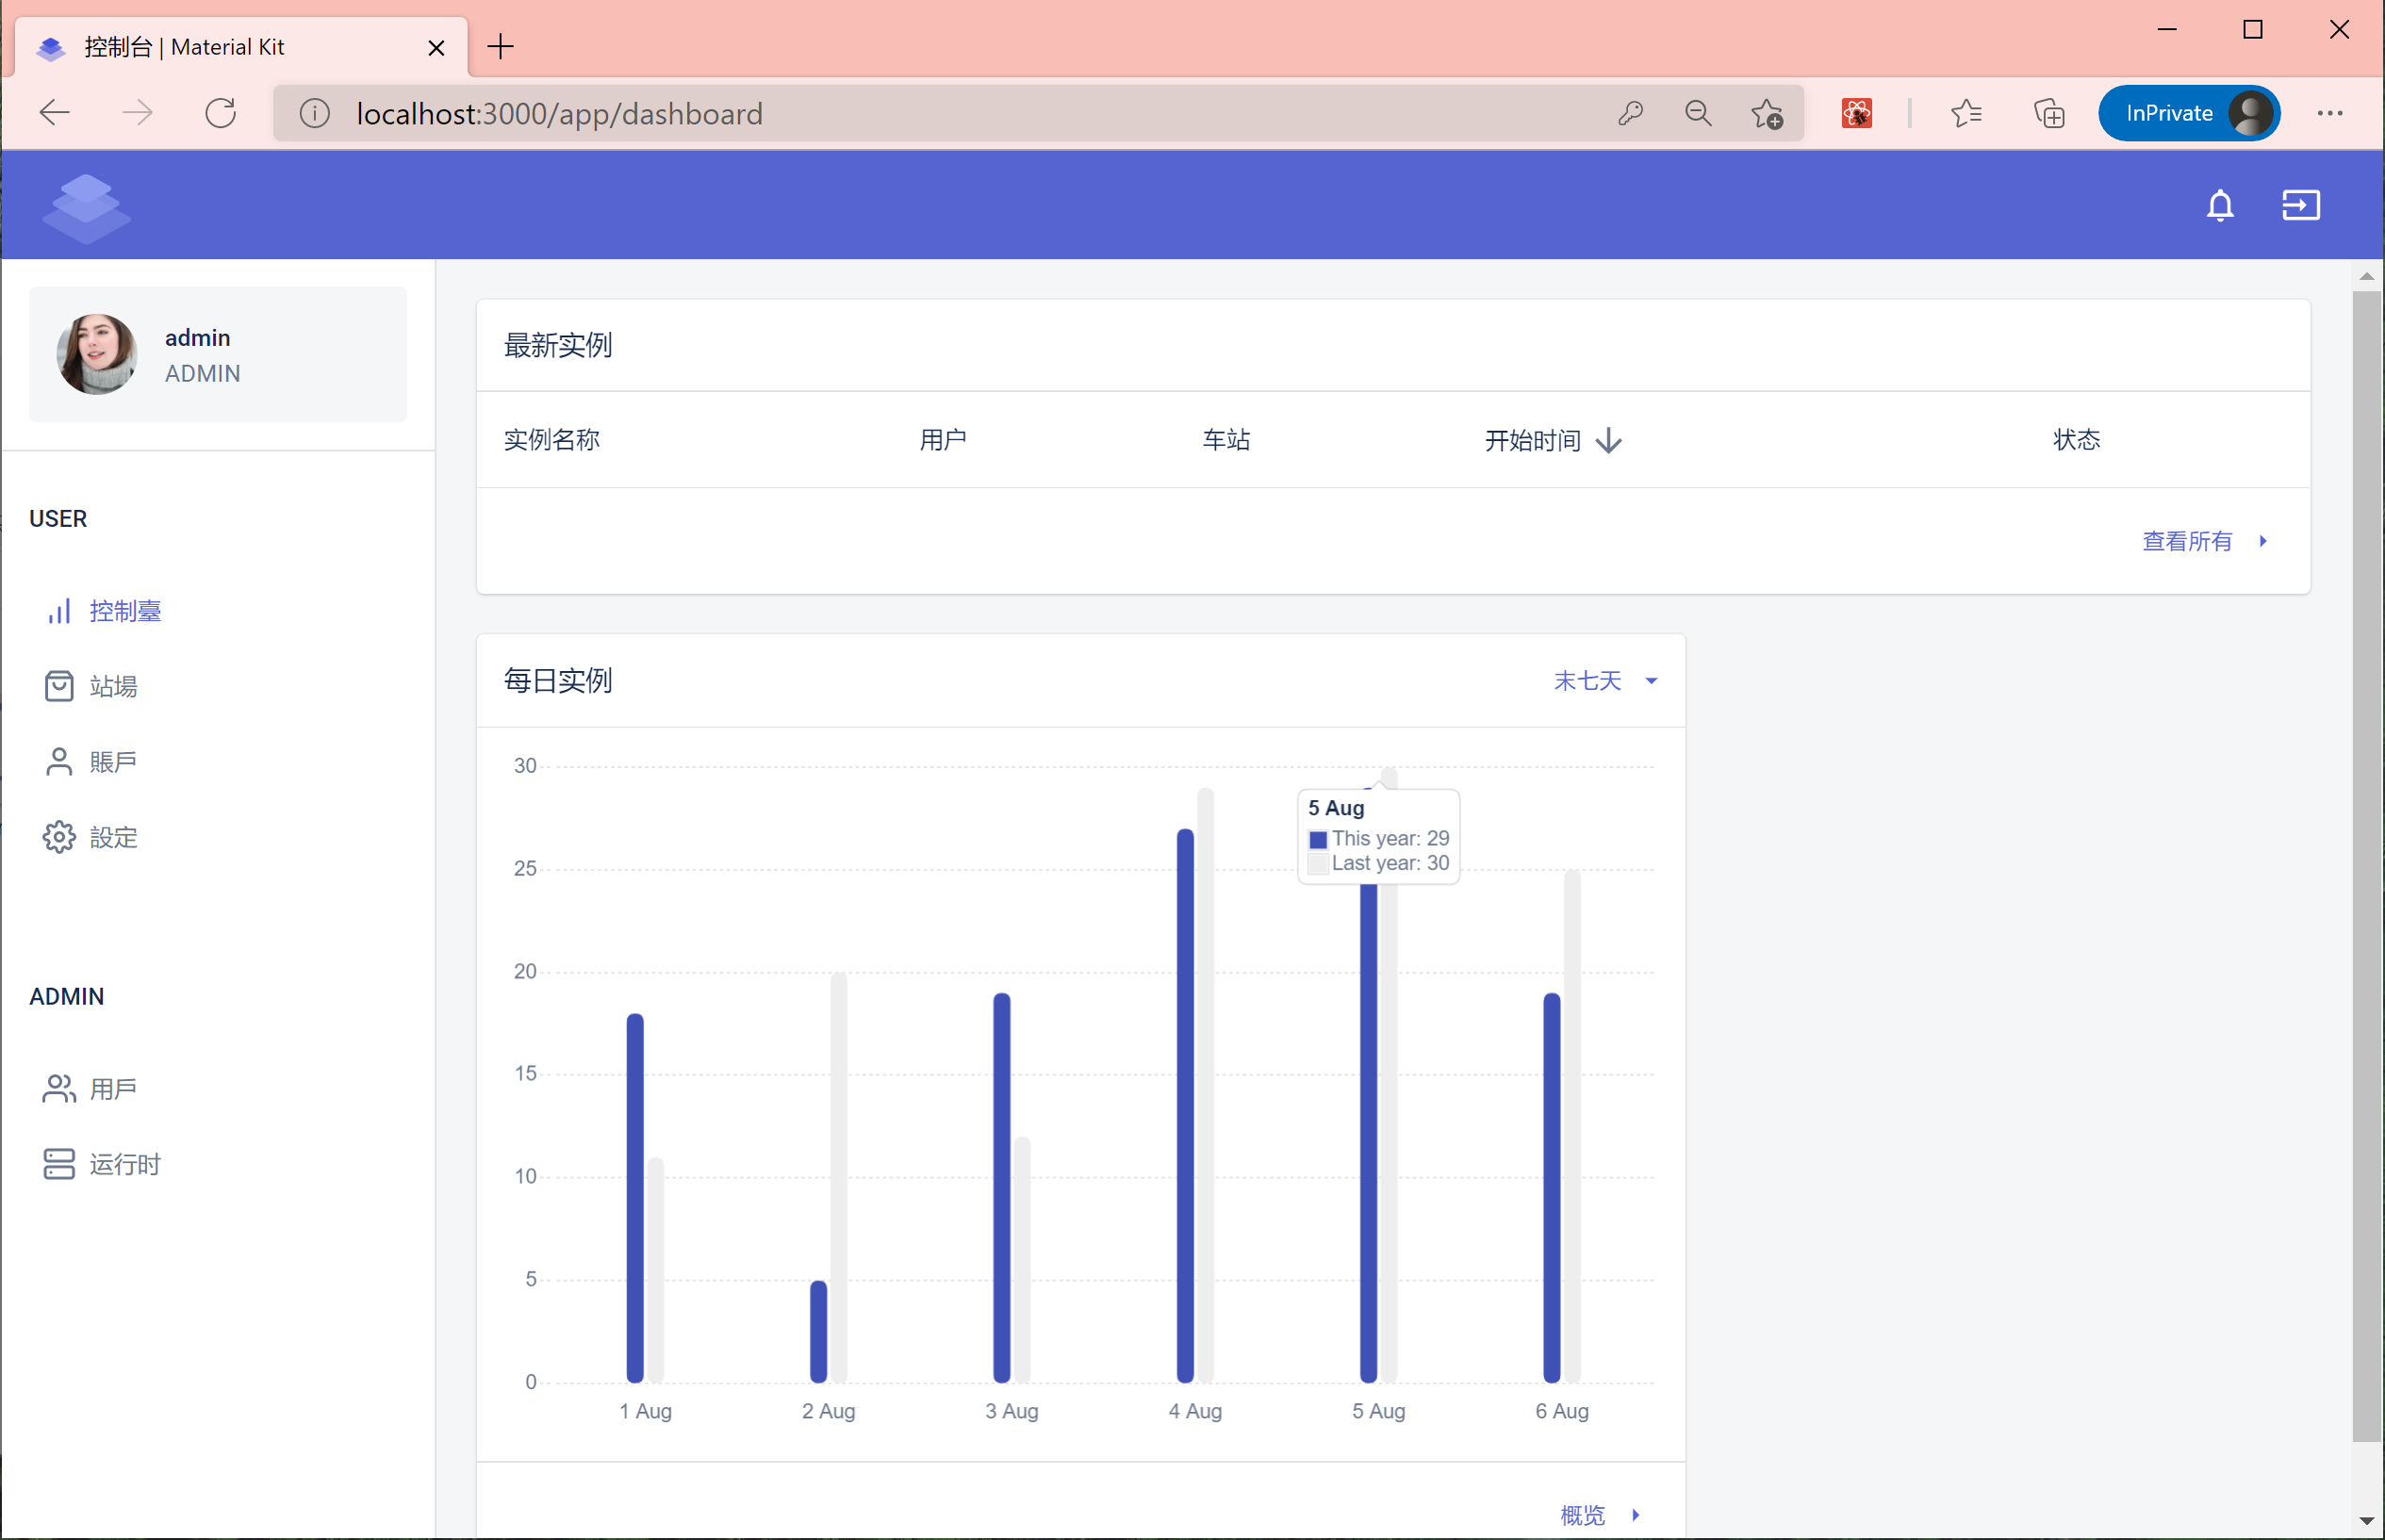
\includegraphics[width=\textwidth]{figures/png/admin_ui.png}
  \caption{\label{admin_ui}管理员角色的控制台首页}
\end{figure}

管理员角色的控制台界面如图\ref{admin_ui} 所示,在侧边栏中是可供用户
点入的功能清单。但与用户角色不同的是,多了用户管理以及运行时管理这两项
只有管理员才有权使用的功能。

\begin{figure}[htbp!]
  \centering
  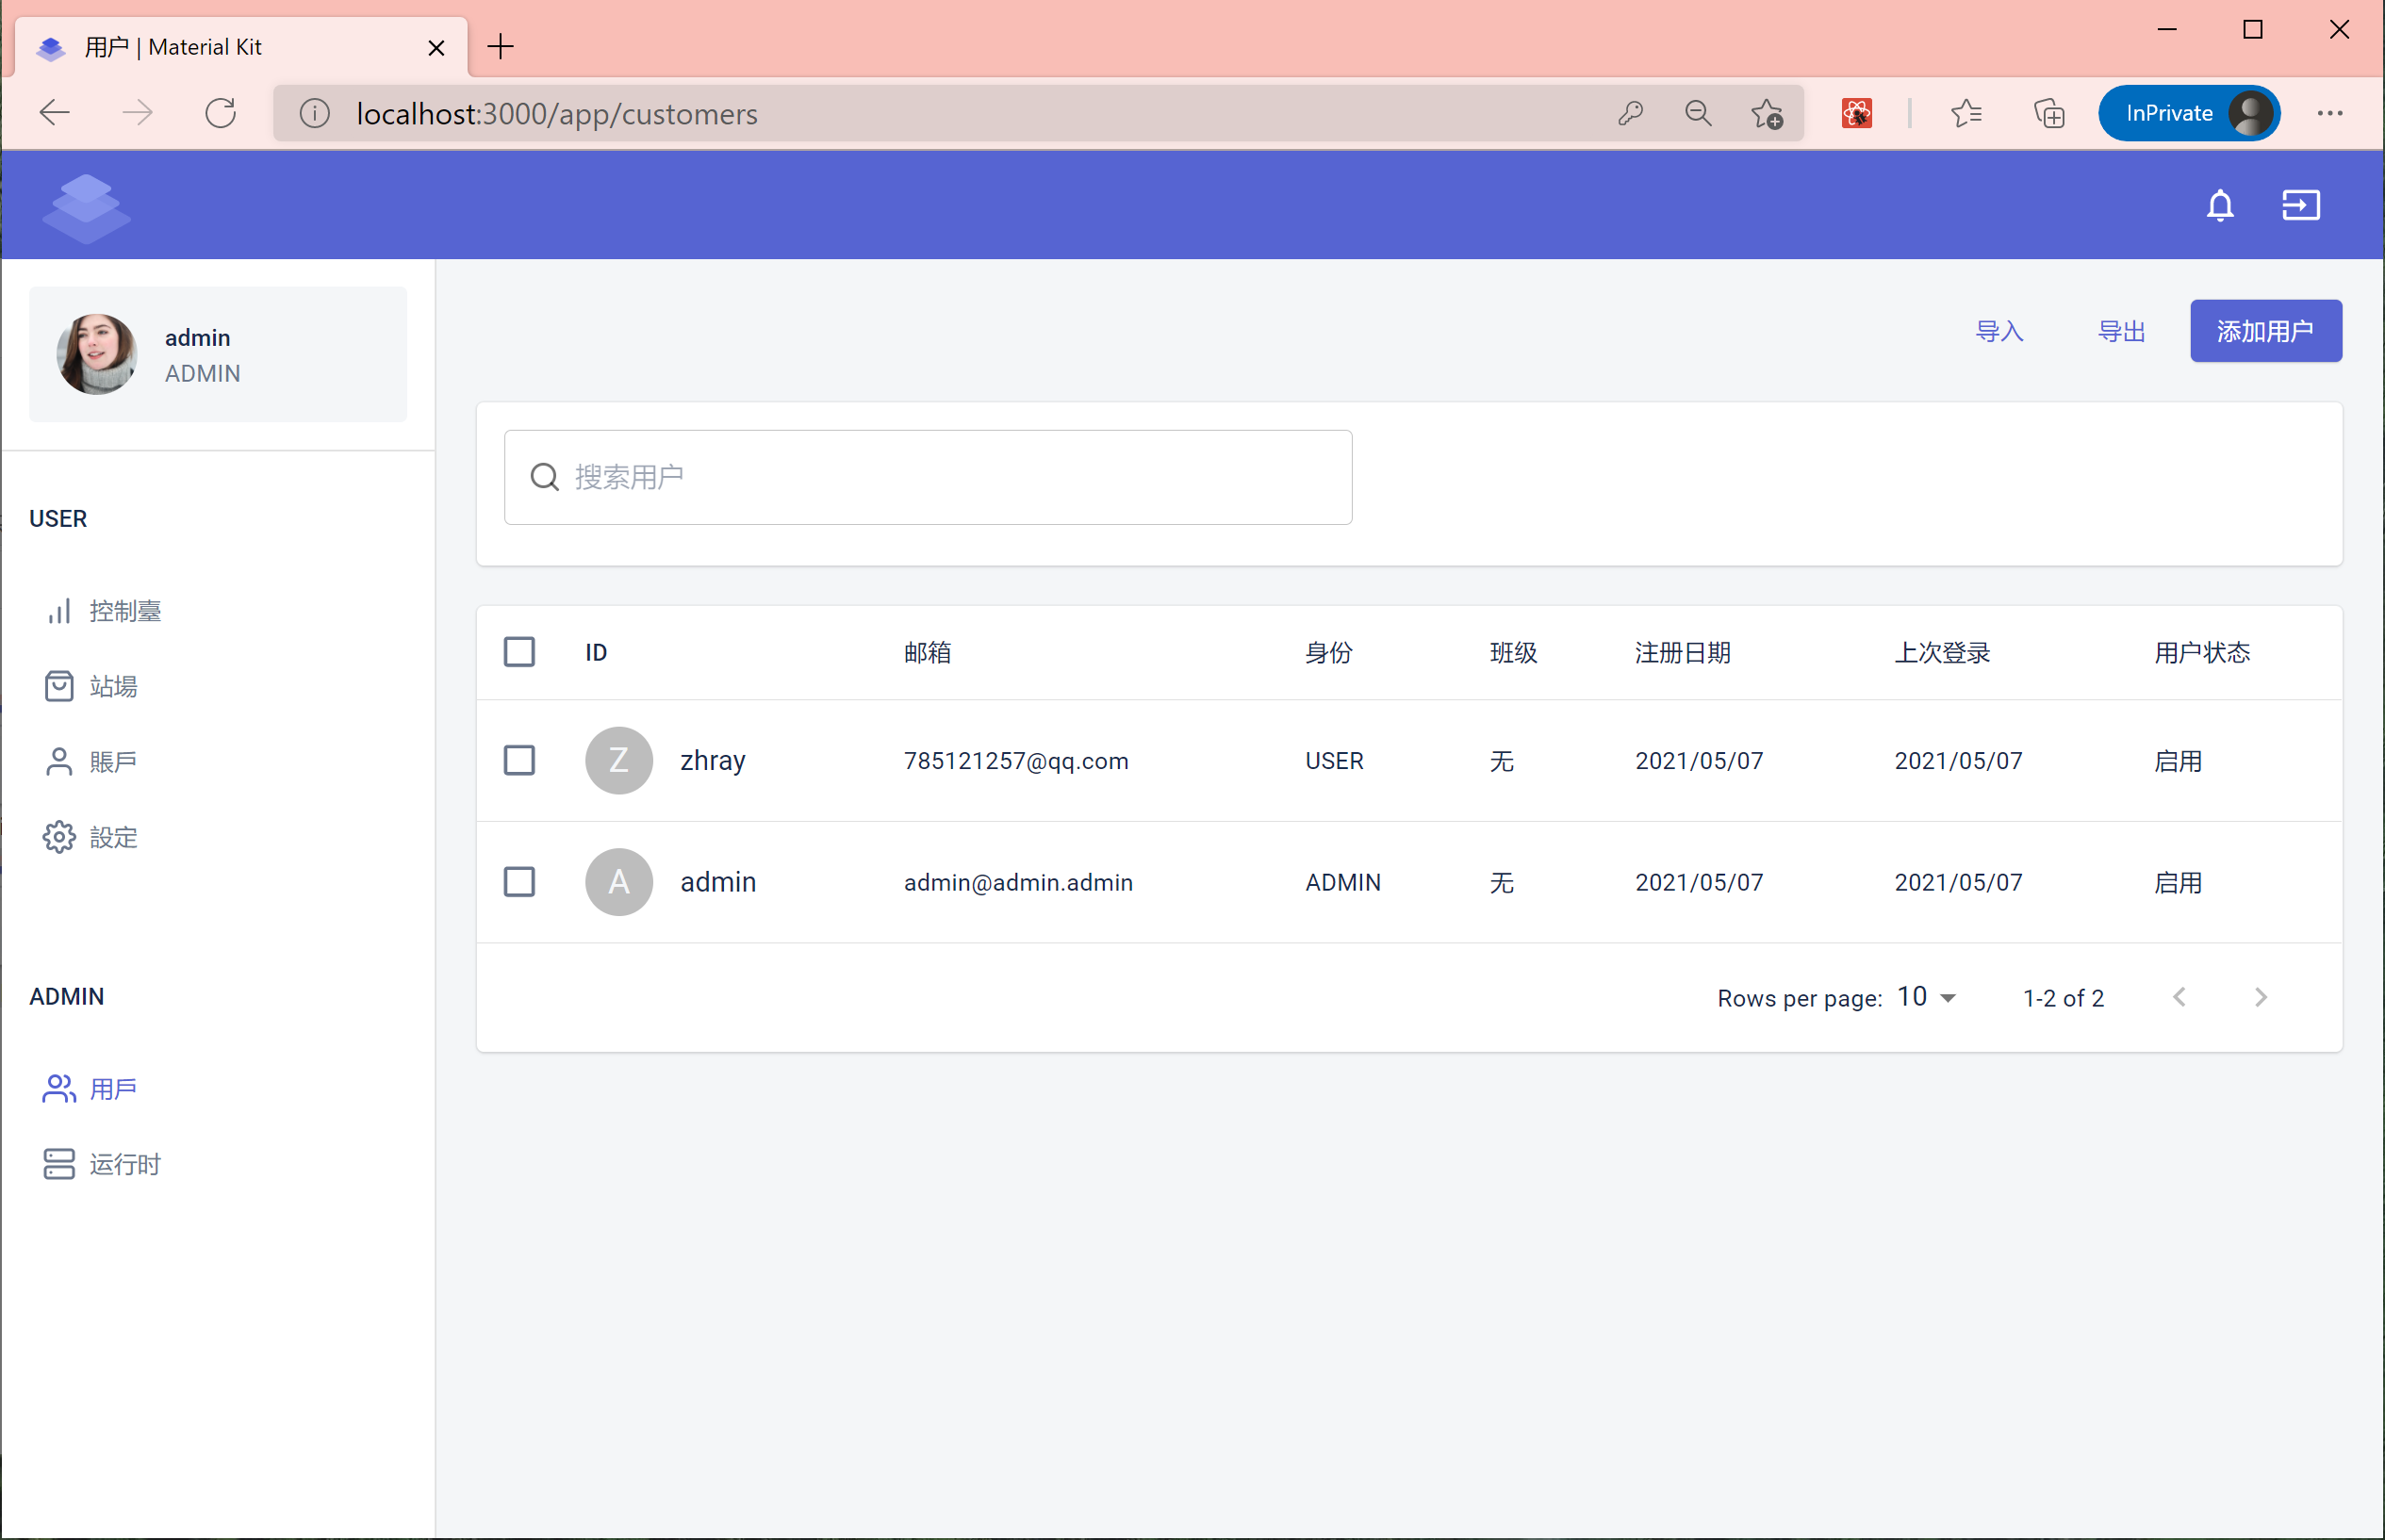
\includegraphics[width=\textwidth]{figures/png/admin_users.png}
  \caption{\label{admin_users}用户管理}
\end{figure}

图\ref{admin_users} 是管理员功能之一的用户管理,从中可以看到刚刚注册成功的zhray账户。

\begin{figure}[htbp!]
  \centering
  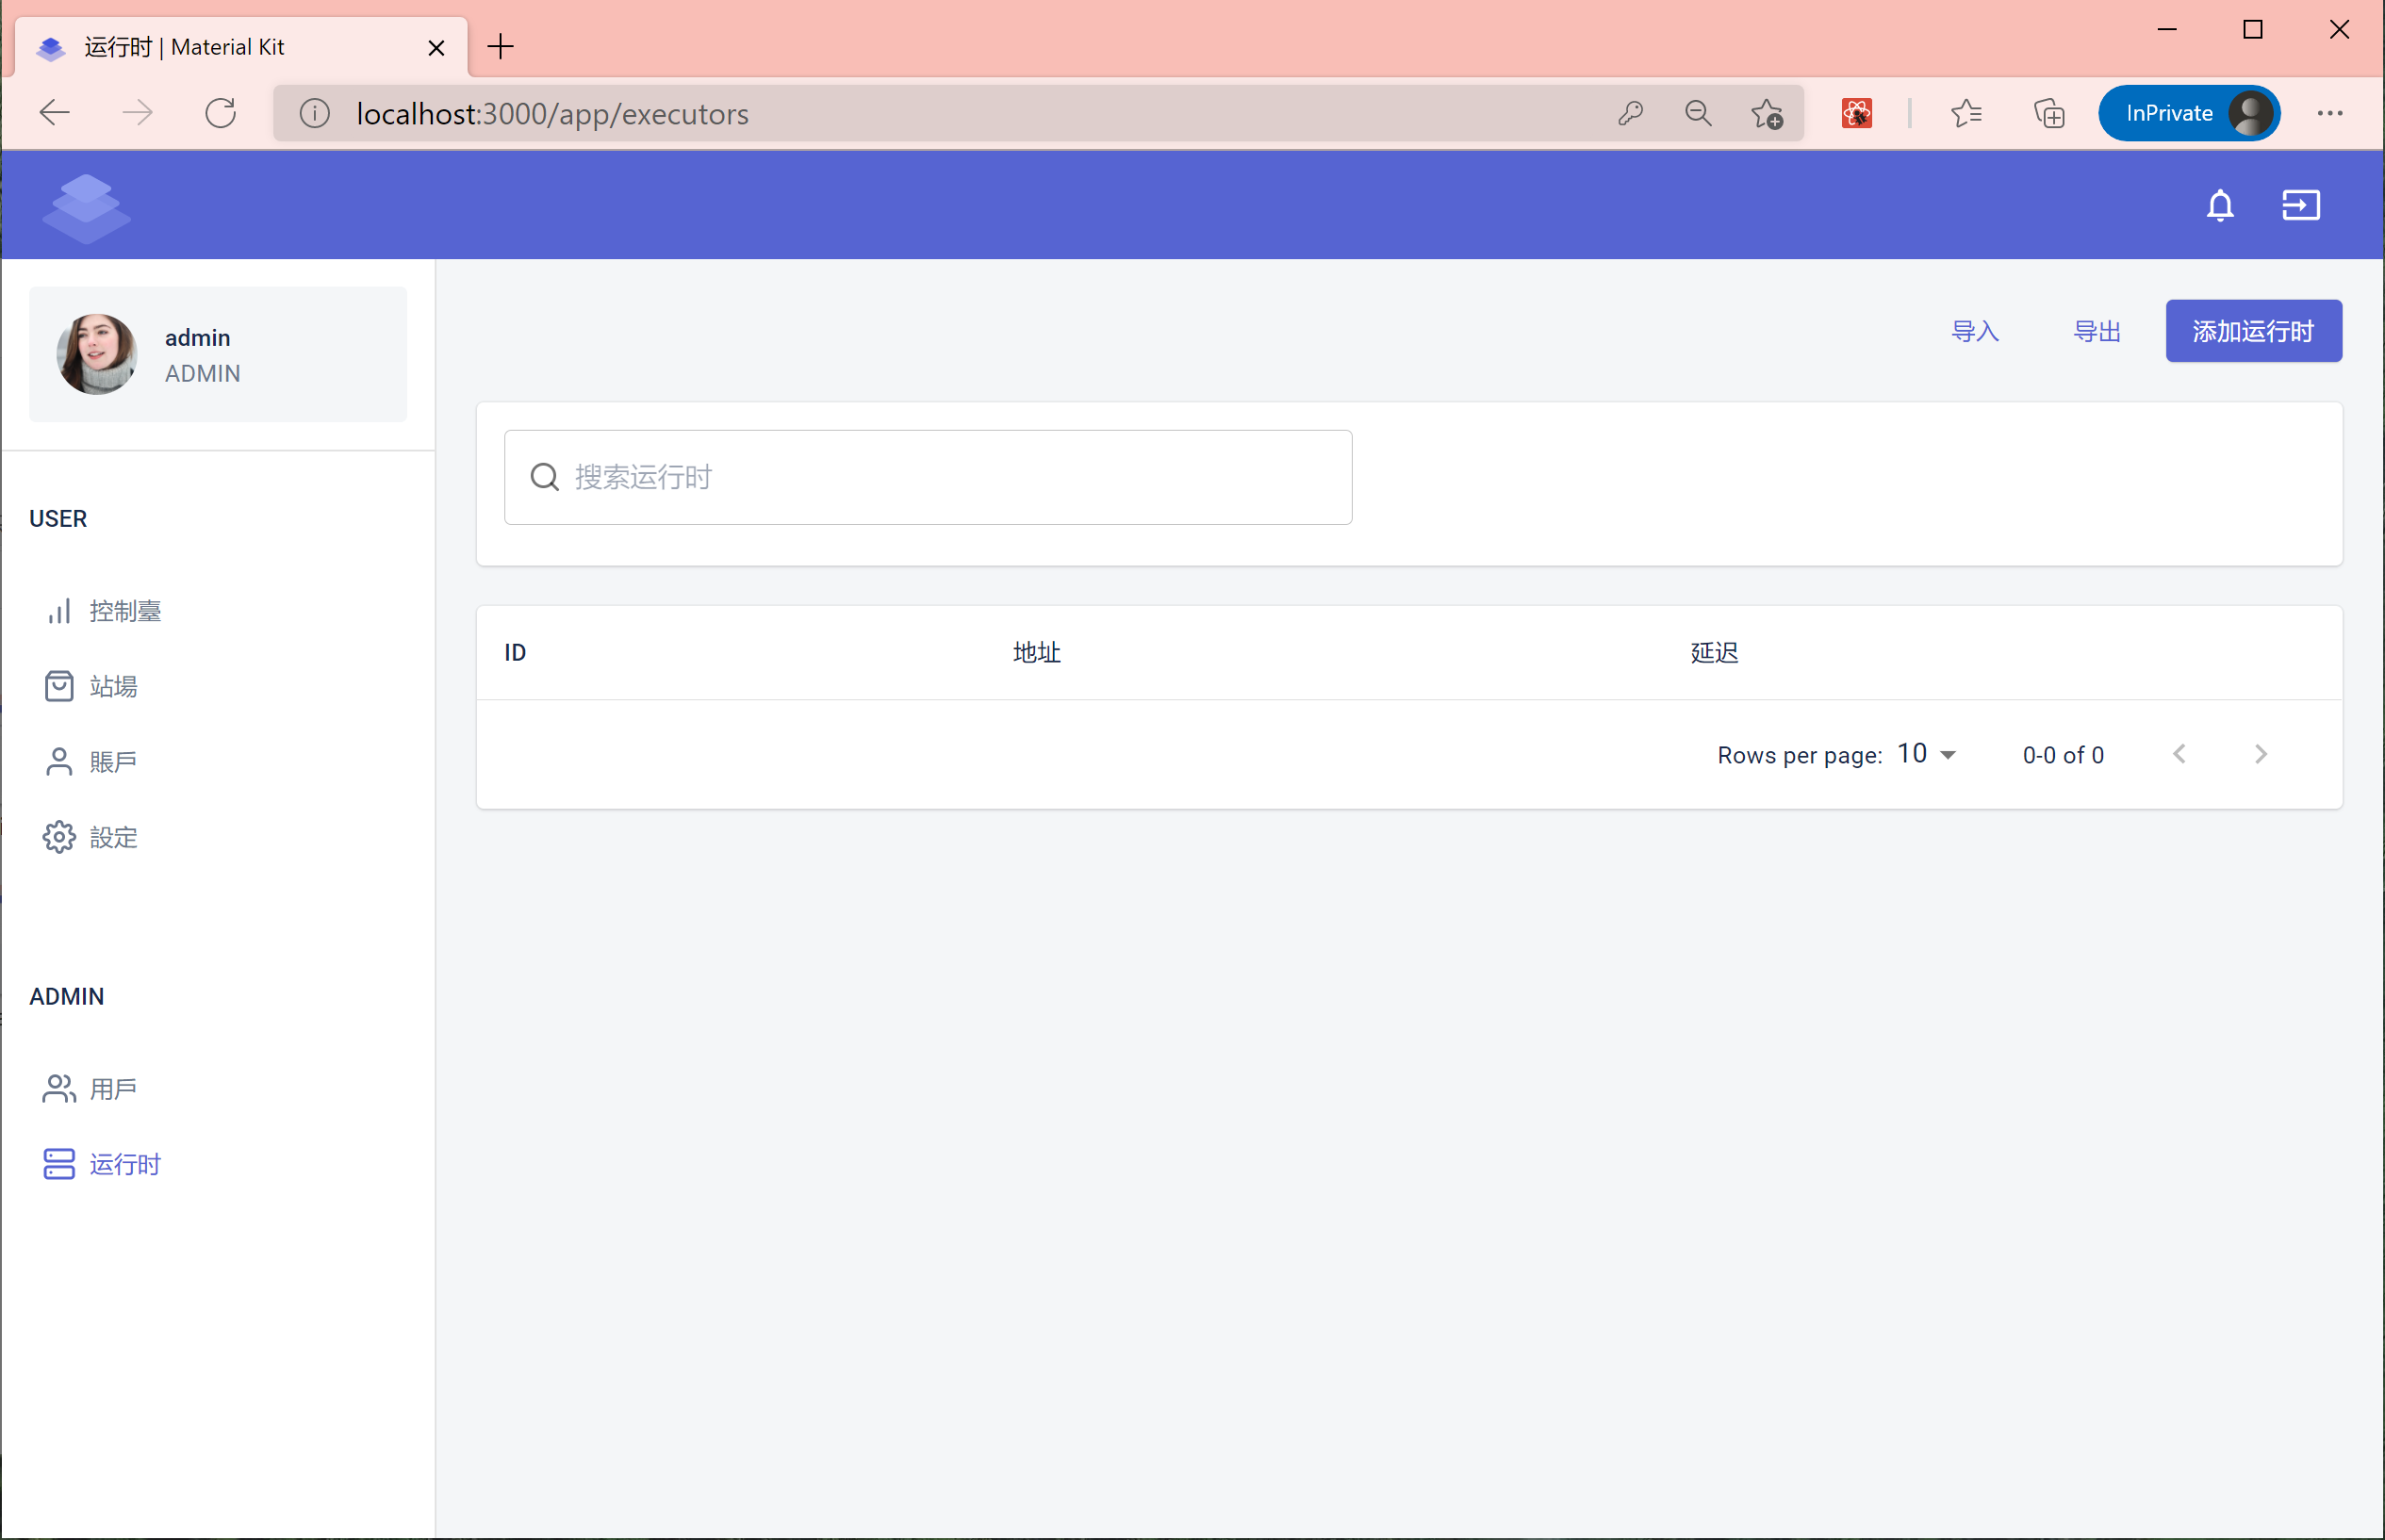
\includegraphics[width=\textwidth]{figures/png/exes.png}
  \caption{\label{exes}运行时管理}
\end{figure}

图\ref{exes} 是管理员功能之一的运行时管理。可以在这里增删改查运行时。

\begin{figure}[htbp!]
  \centering
  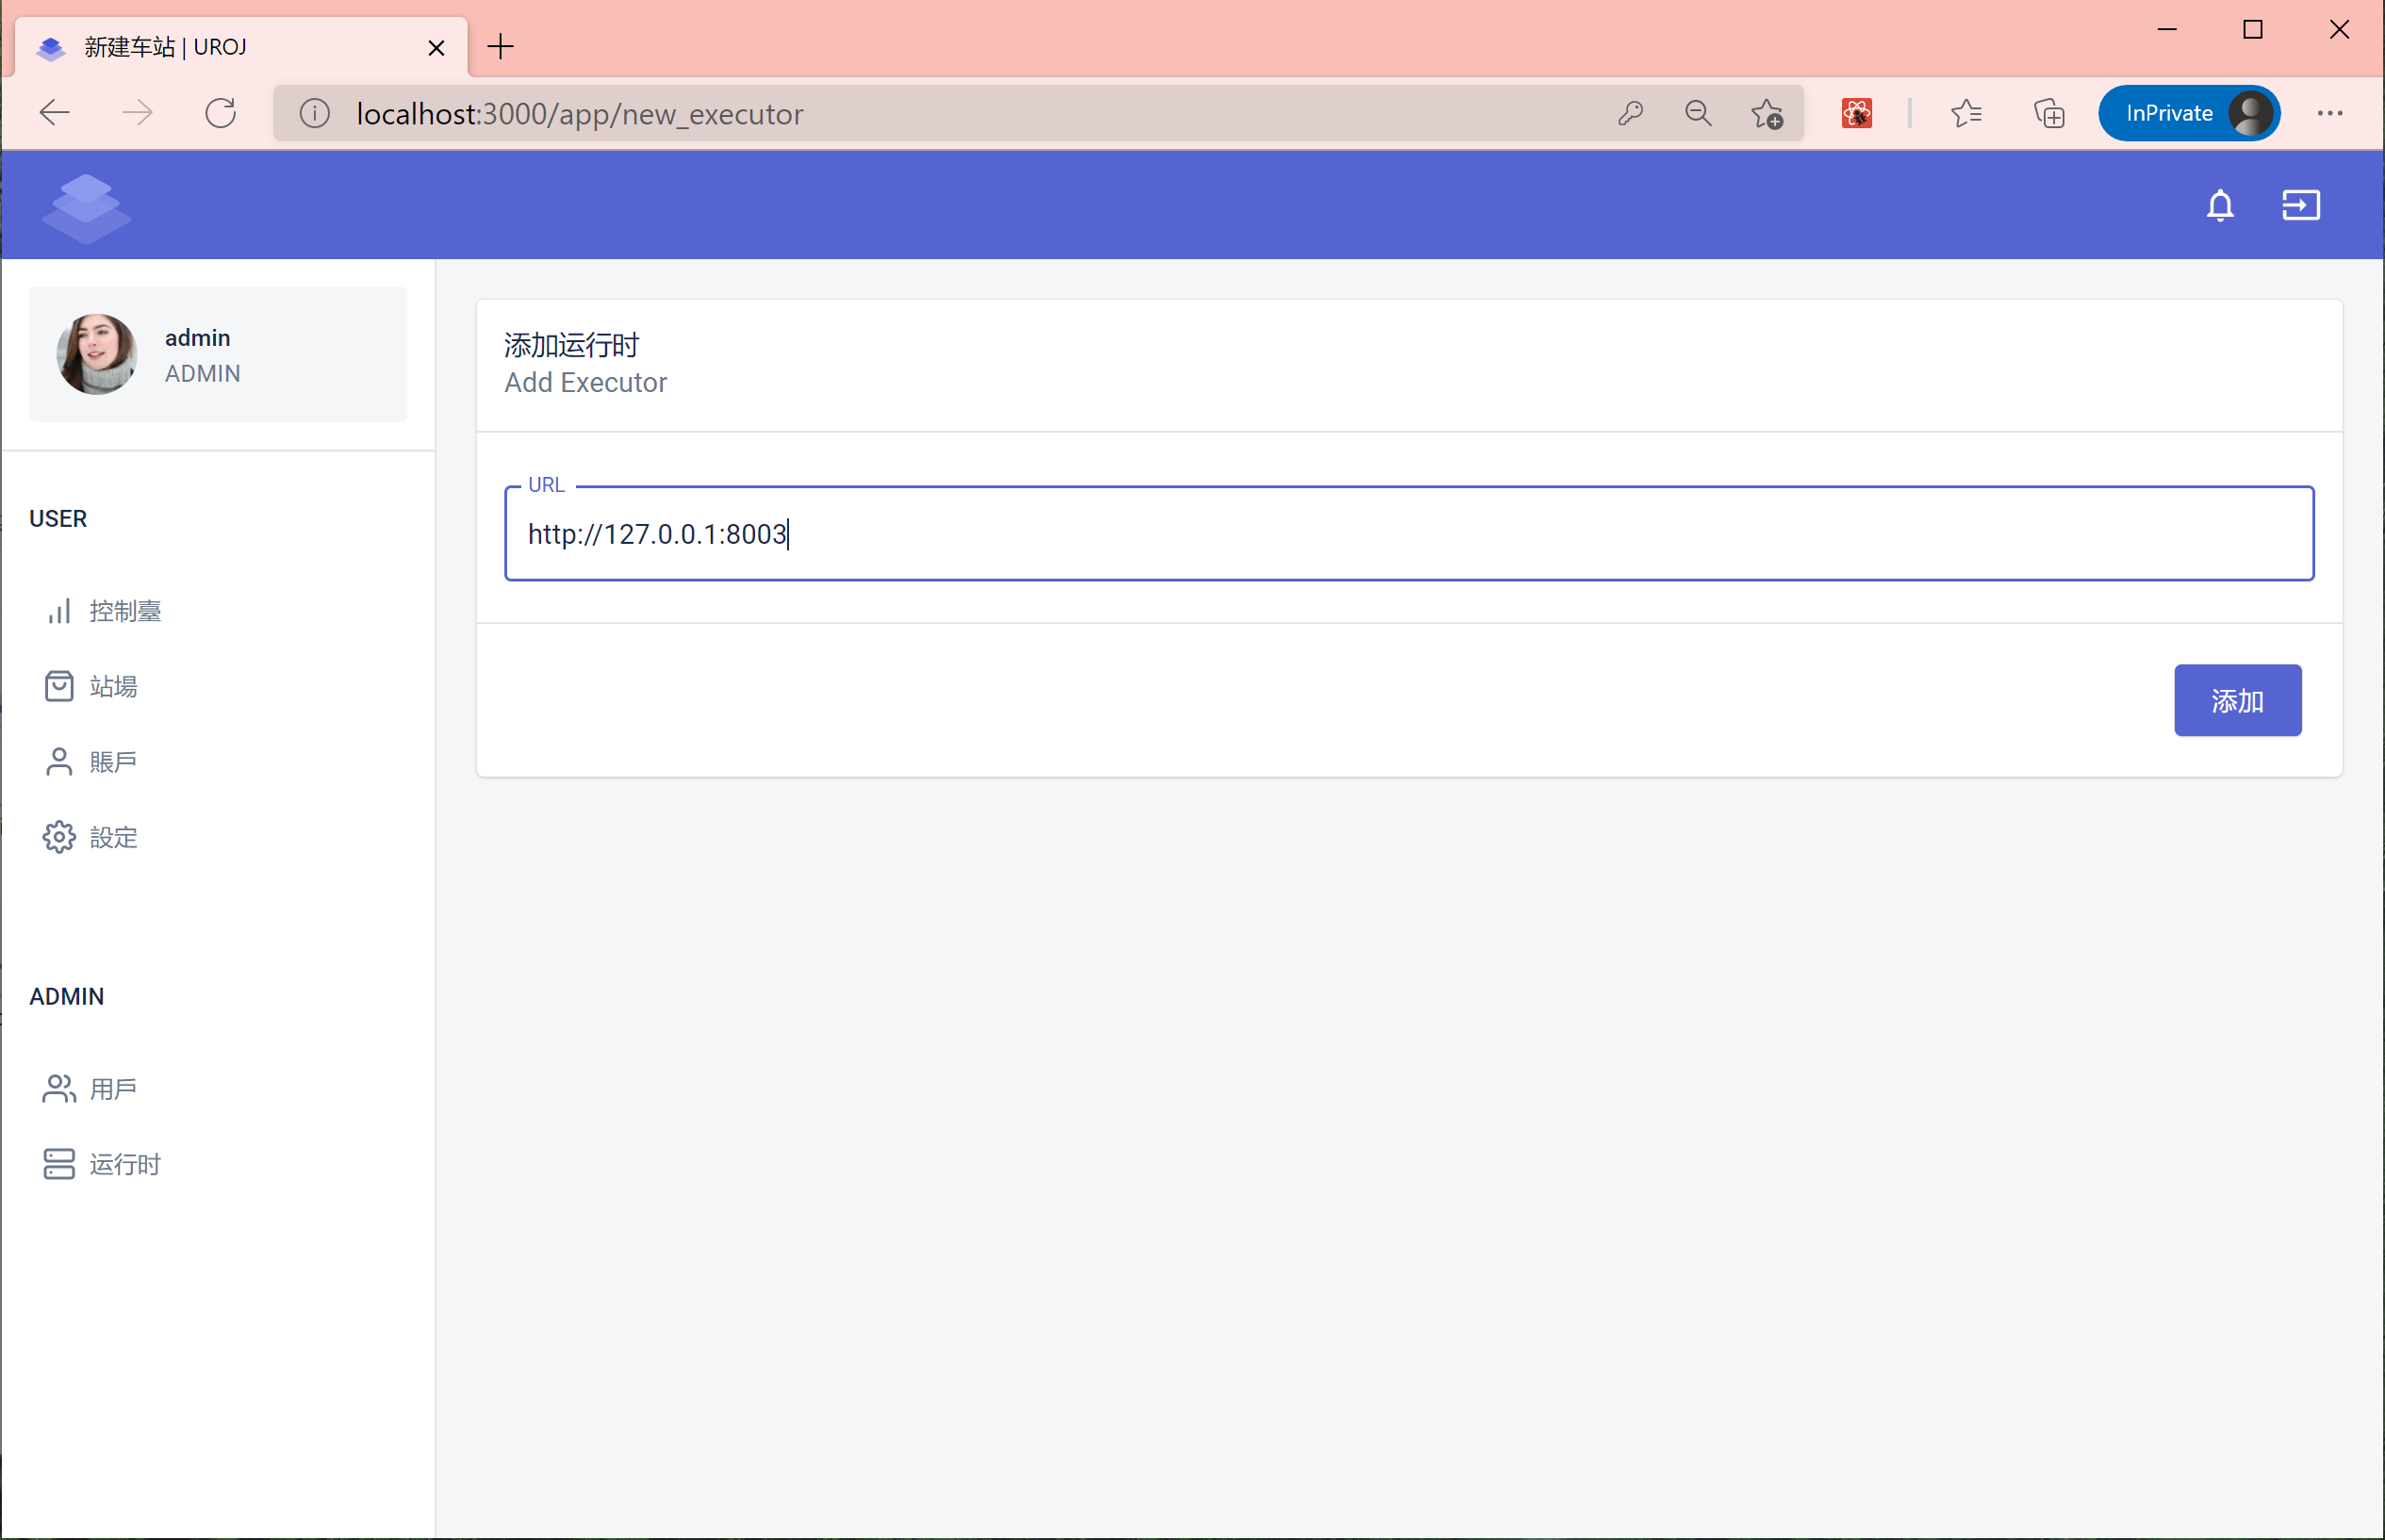
\includegraphics[width=\textwidth]{figures/png/add_exes.png}
  \caption{\label{add_exes}添加运行时}
\end{figure}

\begin{figure}[htbp!]
  \centering
  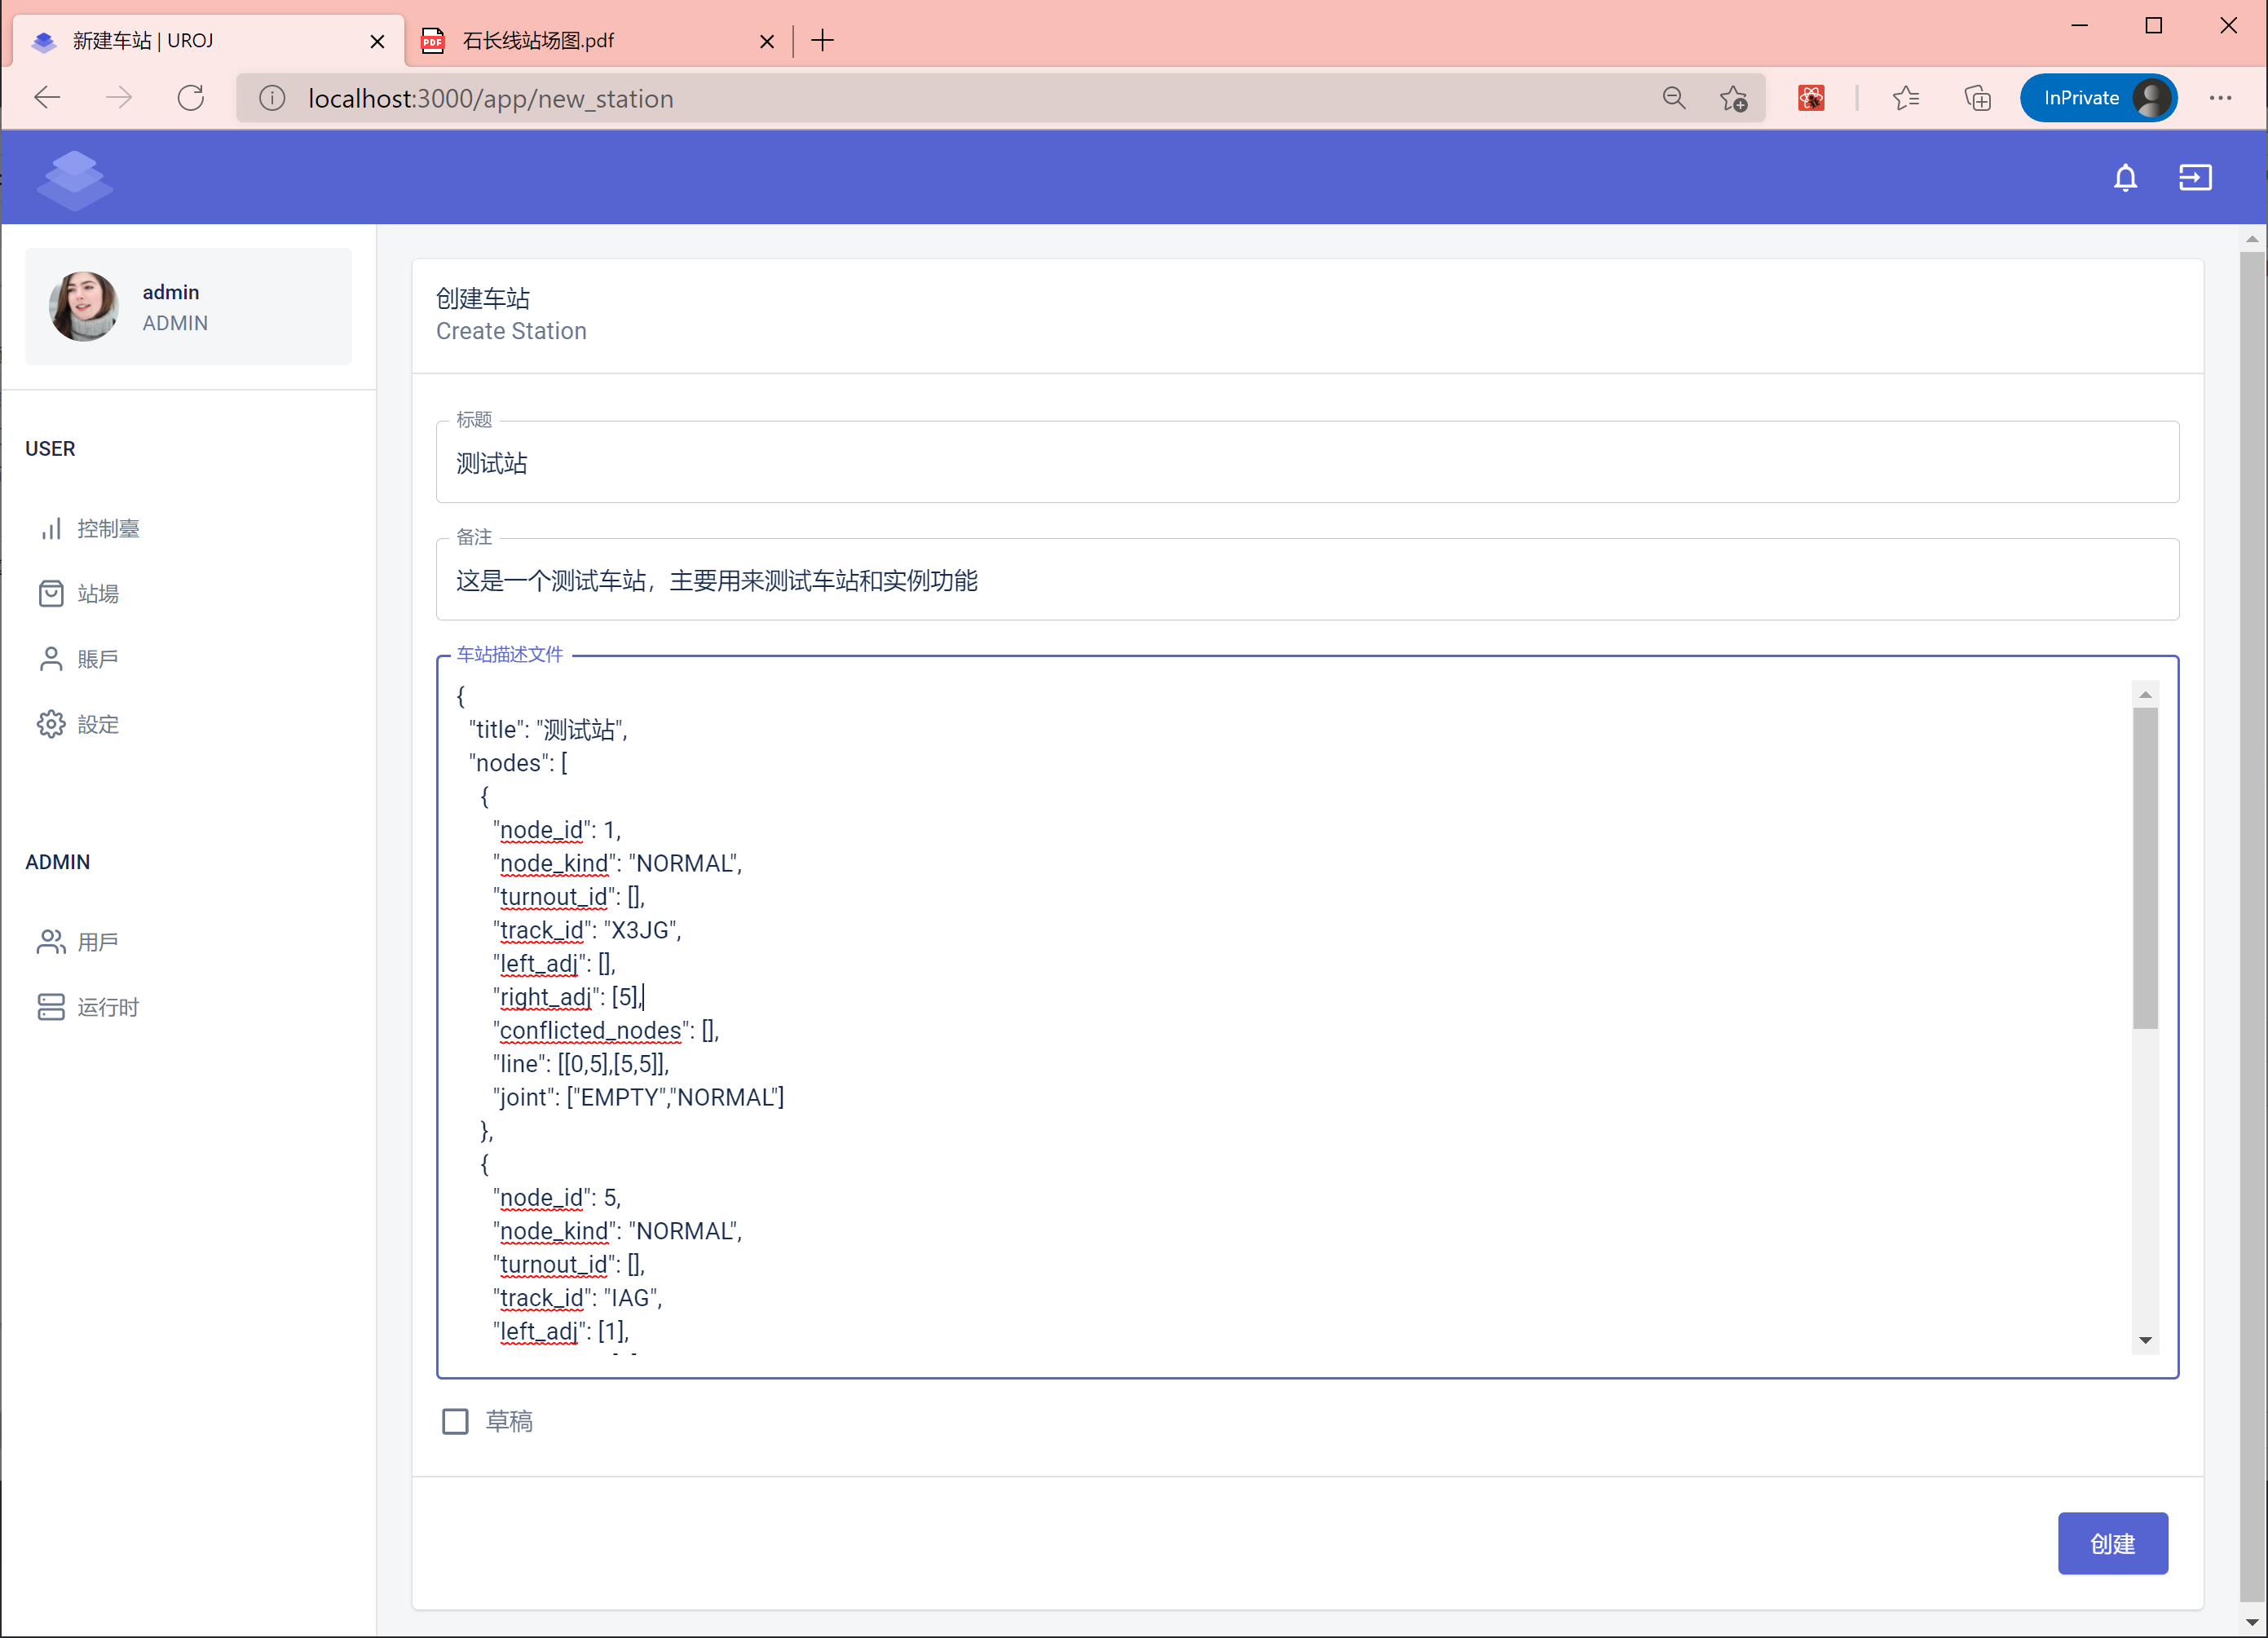
\includegraphics[width=\textwidth]{figures/png/create_sta.png}
  \caption{\label{create_sta}创建车站}
\end{figure}

图\ref{create_sta} 所示的界面是创建车站页面,用户在这里上传车站的相关信息
以及车站描述文件,以新建新车站。

\begin{figure}[htbp!]
  \centering
  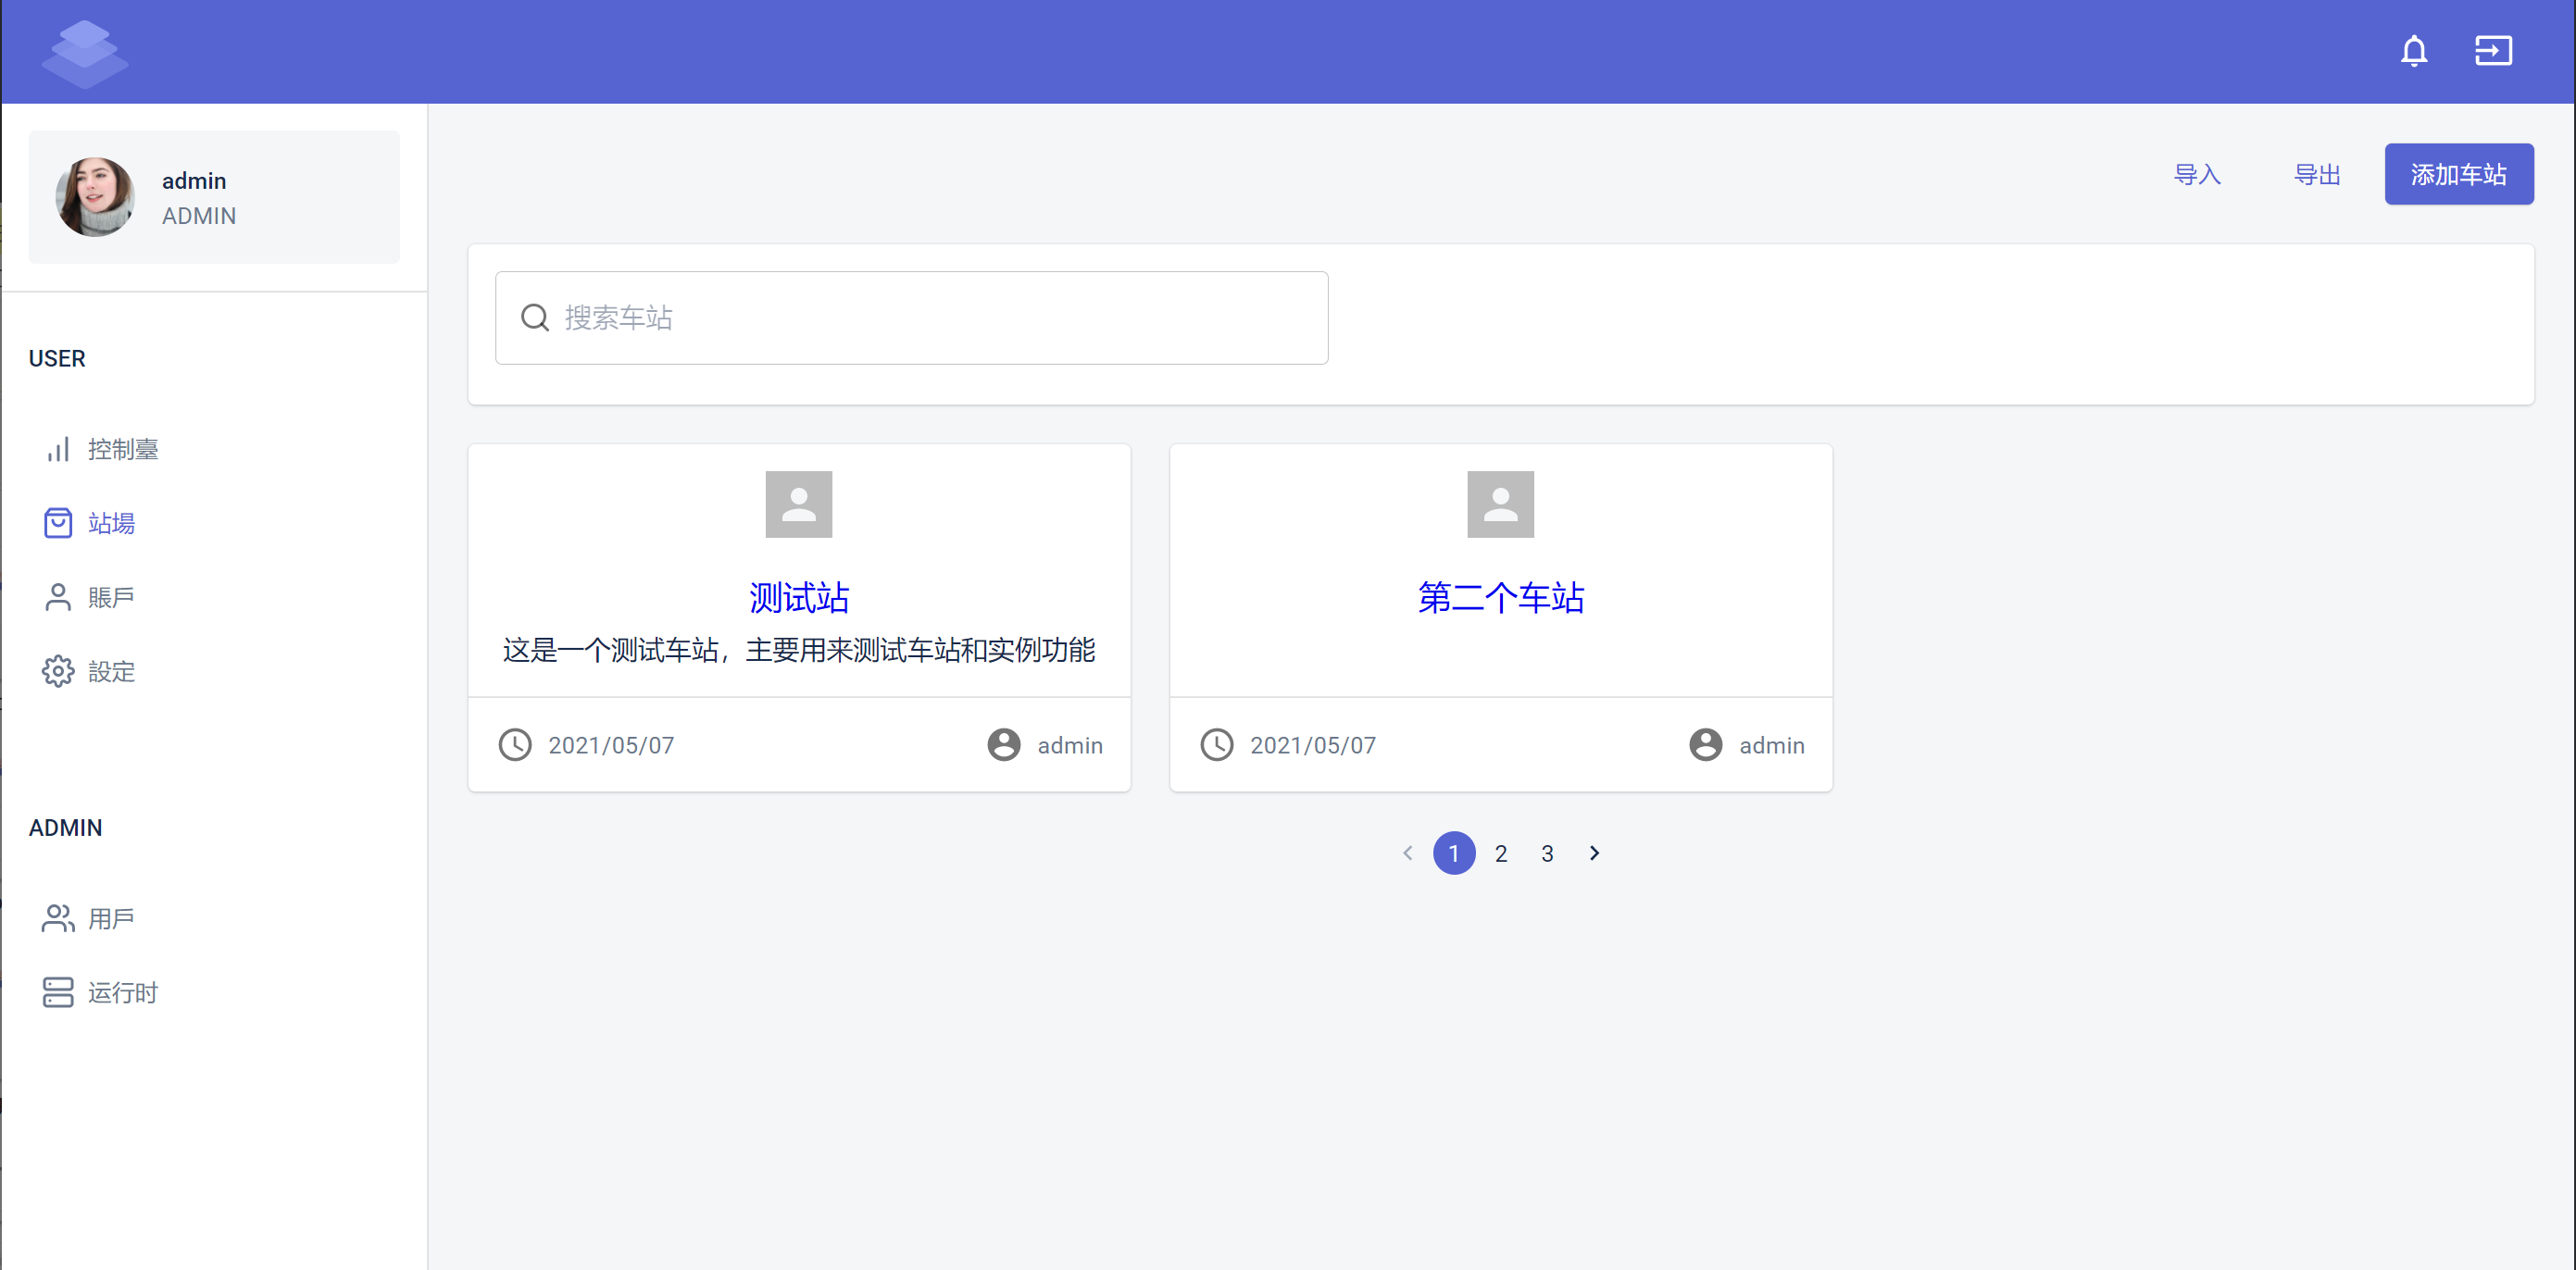
\includegraphics[width=\textwidth]{figures/png/station_list.png}
  \caption{\label{station_list}车站页面}
\end{figure}

图\ref{station_list} 所示页面为车站列表页面,其列出了当前系统中所有
的车站。

\begin{figure}[htbp!]
  \centering
  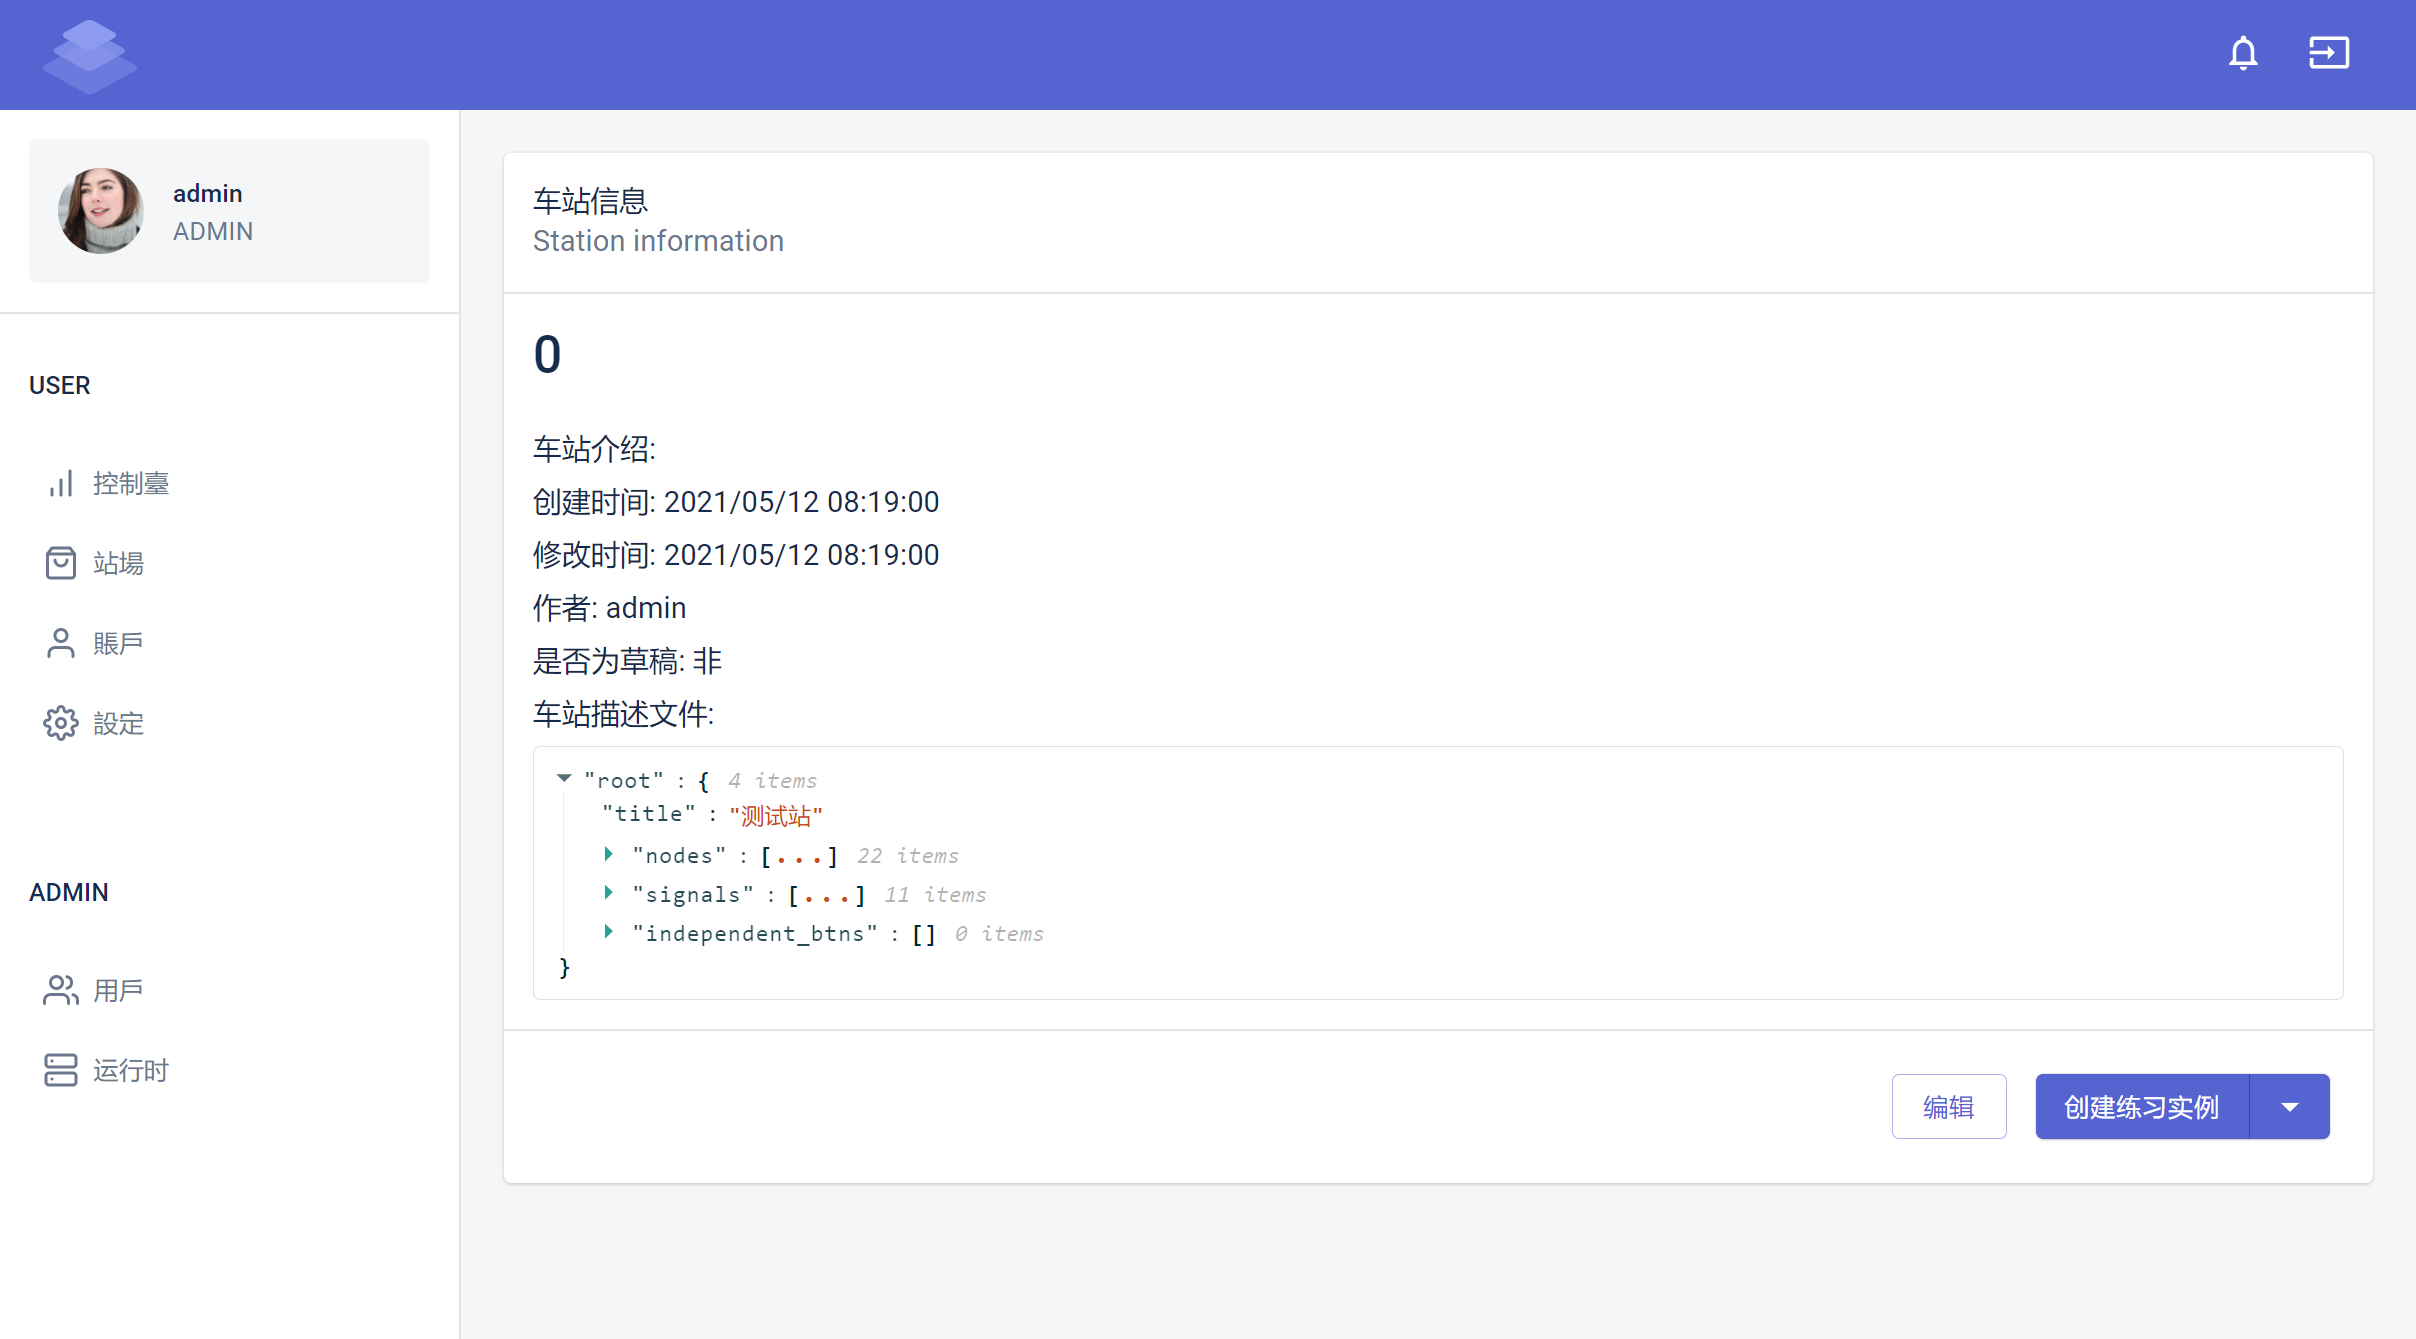
\includegraphics[width=\textwidth]{figures/png/station_info.png}
  \caption{\label{station_info}车站信息查看}
\end{figure}

图\ref{station_info} 所示的页面为车站的详情页面,显示着某个车站的所有信息。
其中为车站描述文件显示称为可交互的树状图,方便用户查看,提升用户体验。

\begin{figure}[htbp!]
  \centering
  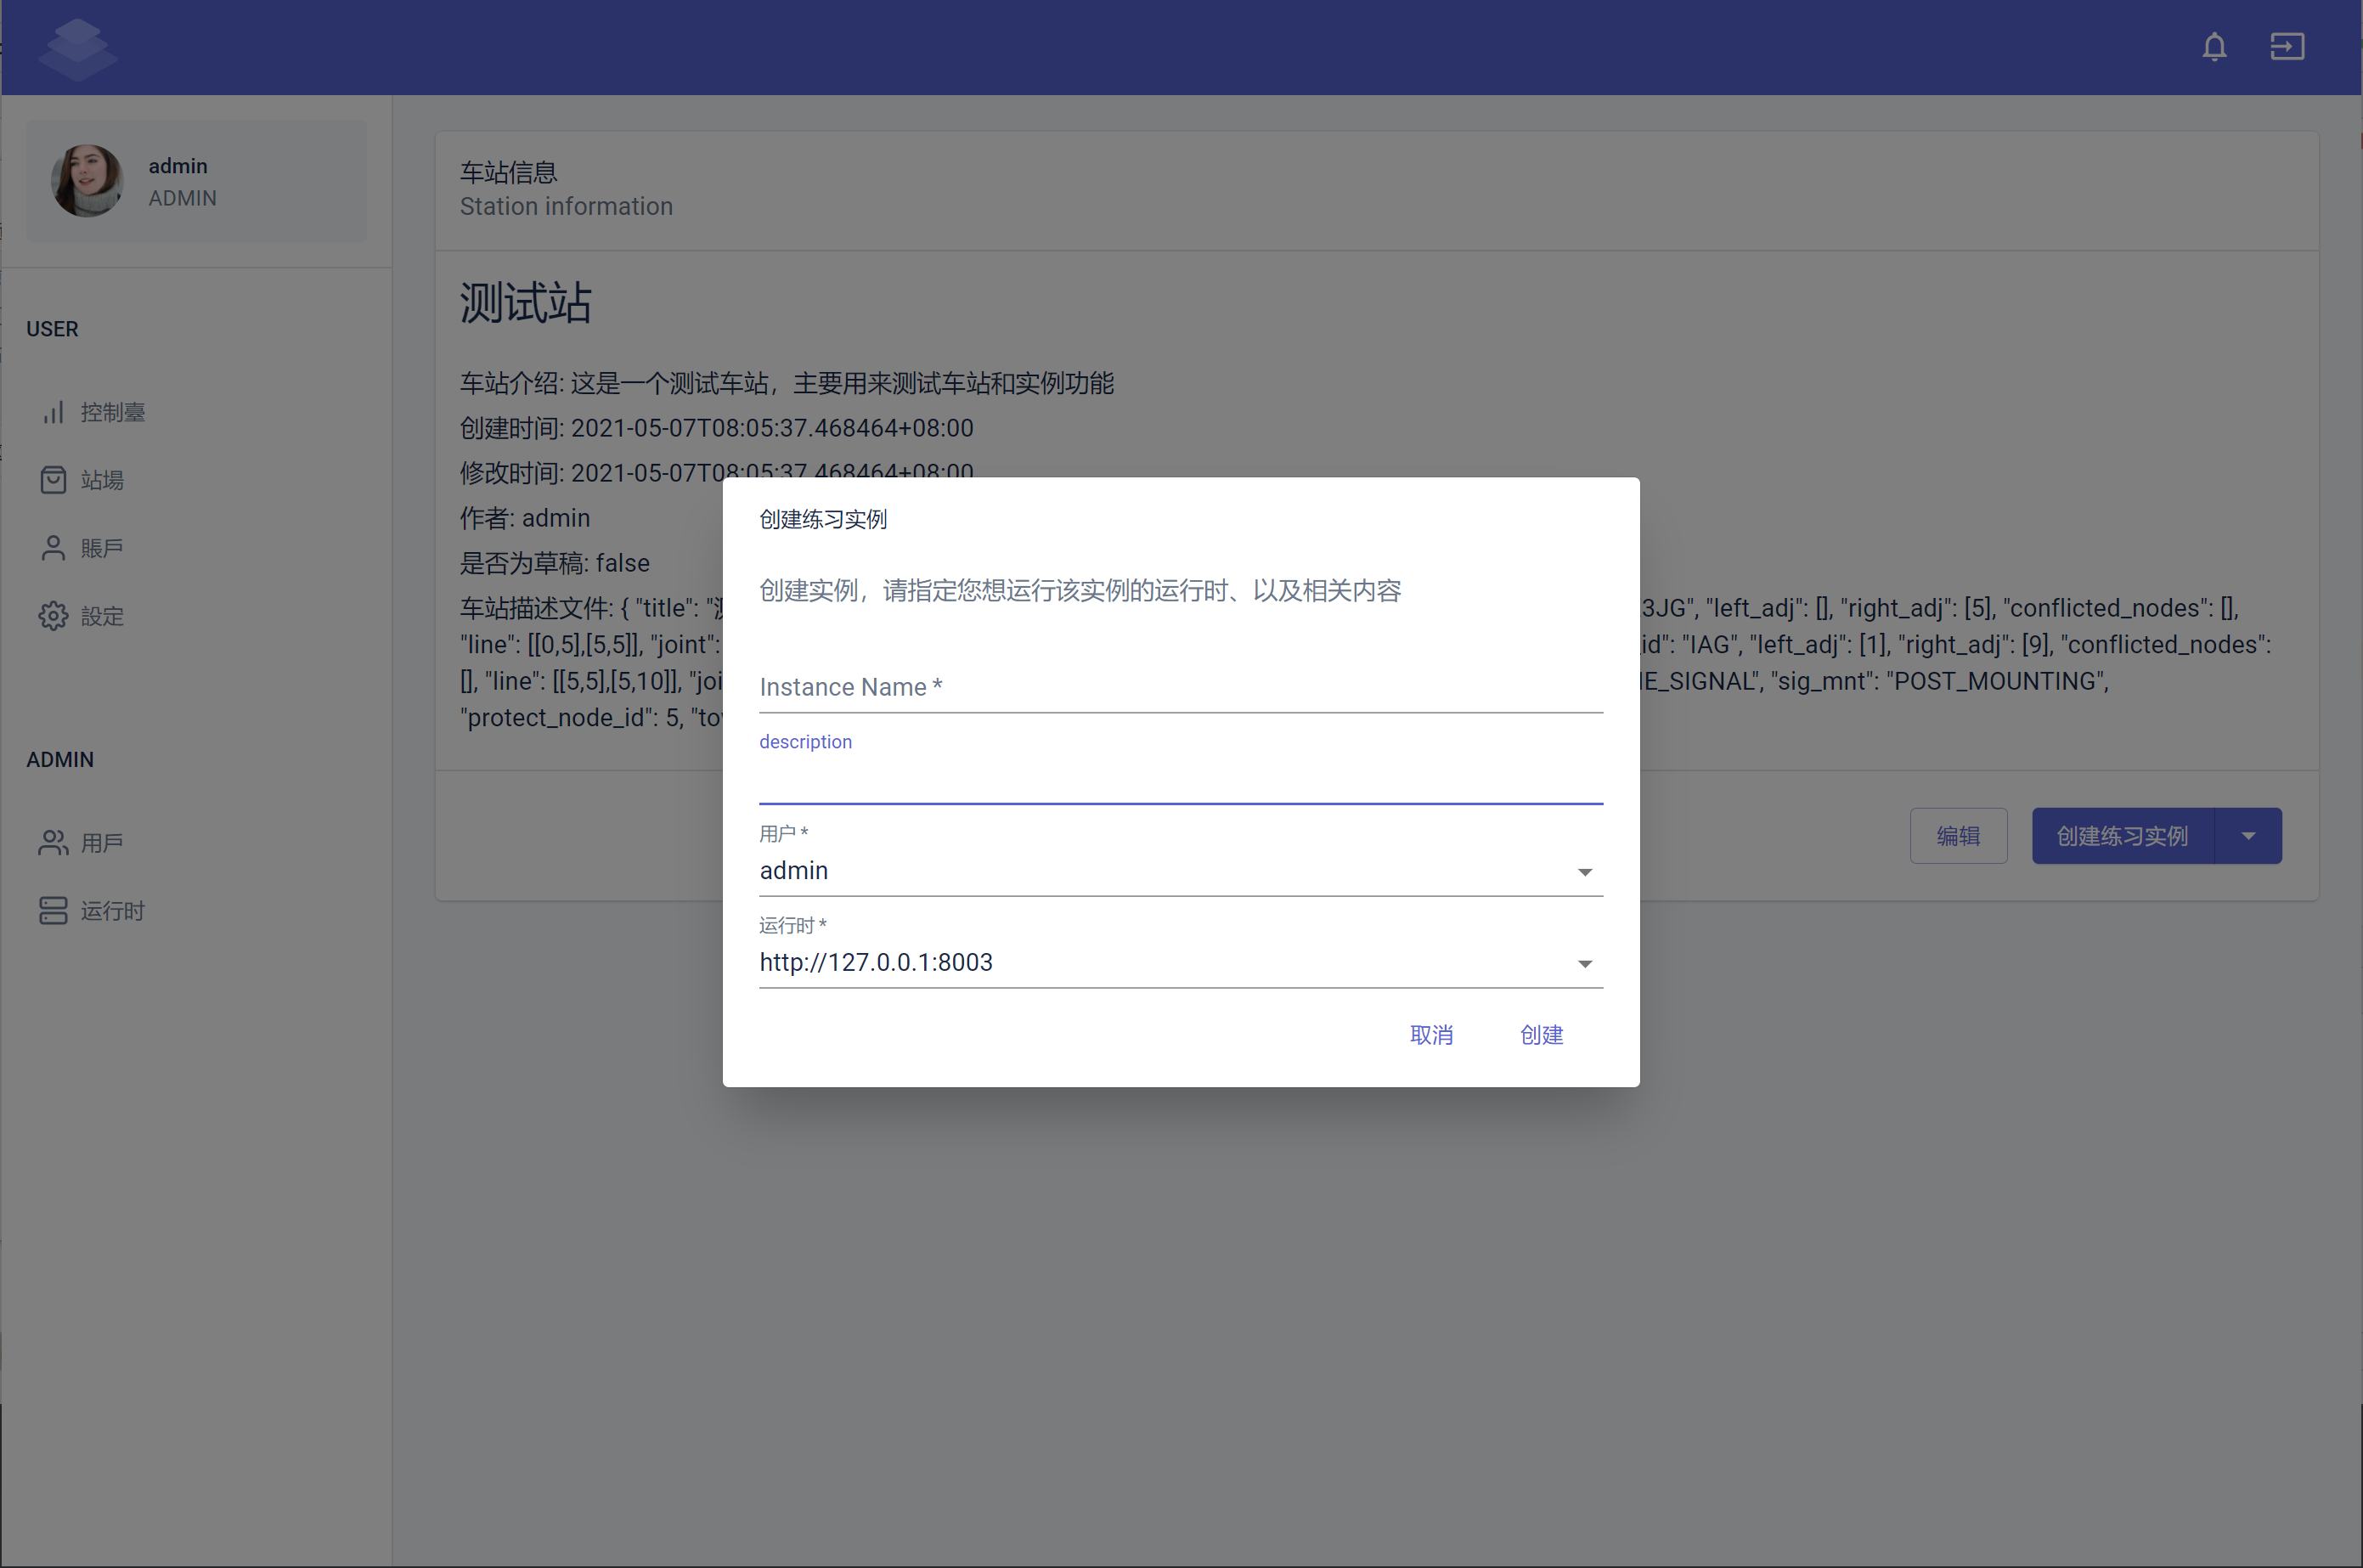
\includegraphics[width=\textwidth]{figures/png/dialog.png}
  \caption{\label{dialog}新建实例对话框}
\end{figure}

点击右下角的按钮后会弹出如图\ref{dialog} 所示的对话框,
用户使用该对话框新建实例。其中用户选单和运行时选单中的数据是从服务器中
获取的所有用户和所有运行时清单,供用户在新建实例时选择。

\begin{figure}[htbp!]
  \centering
  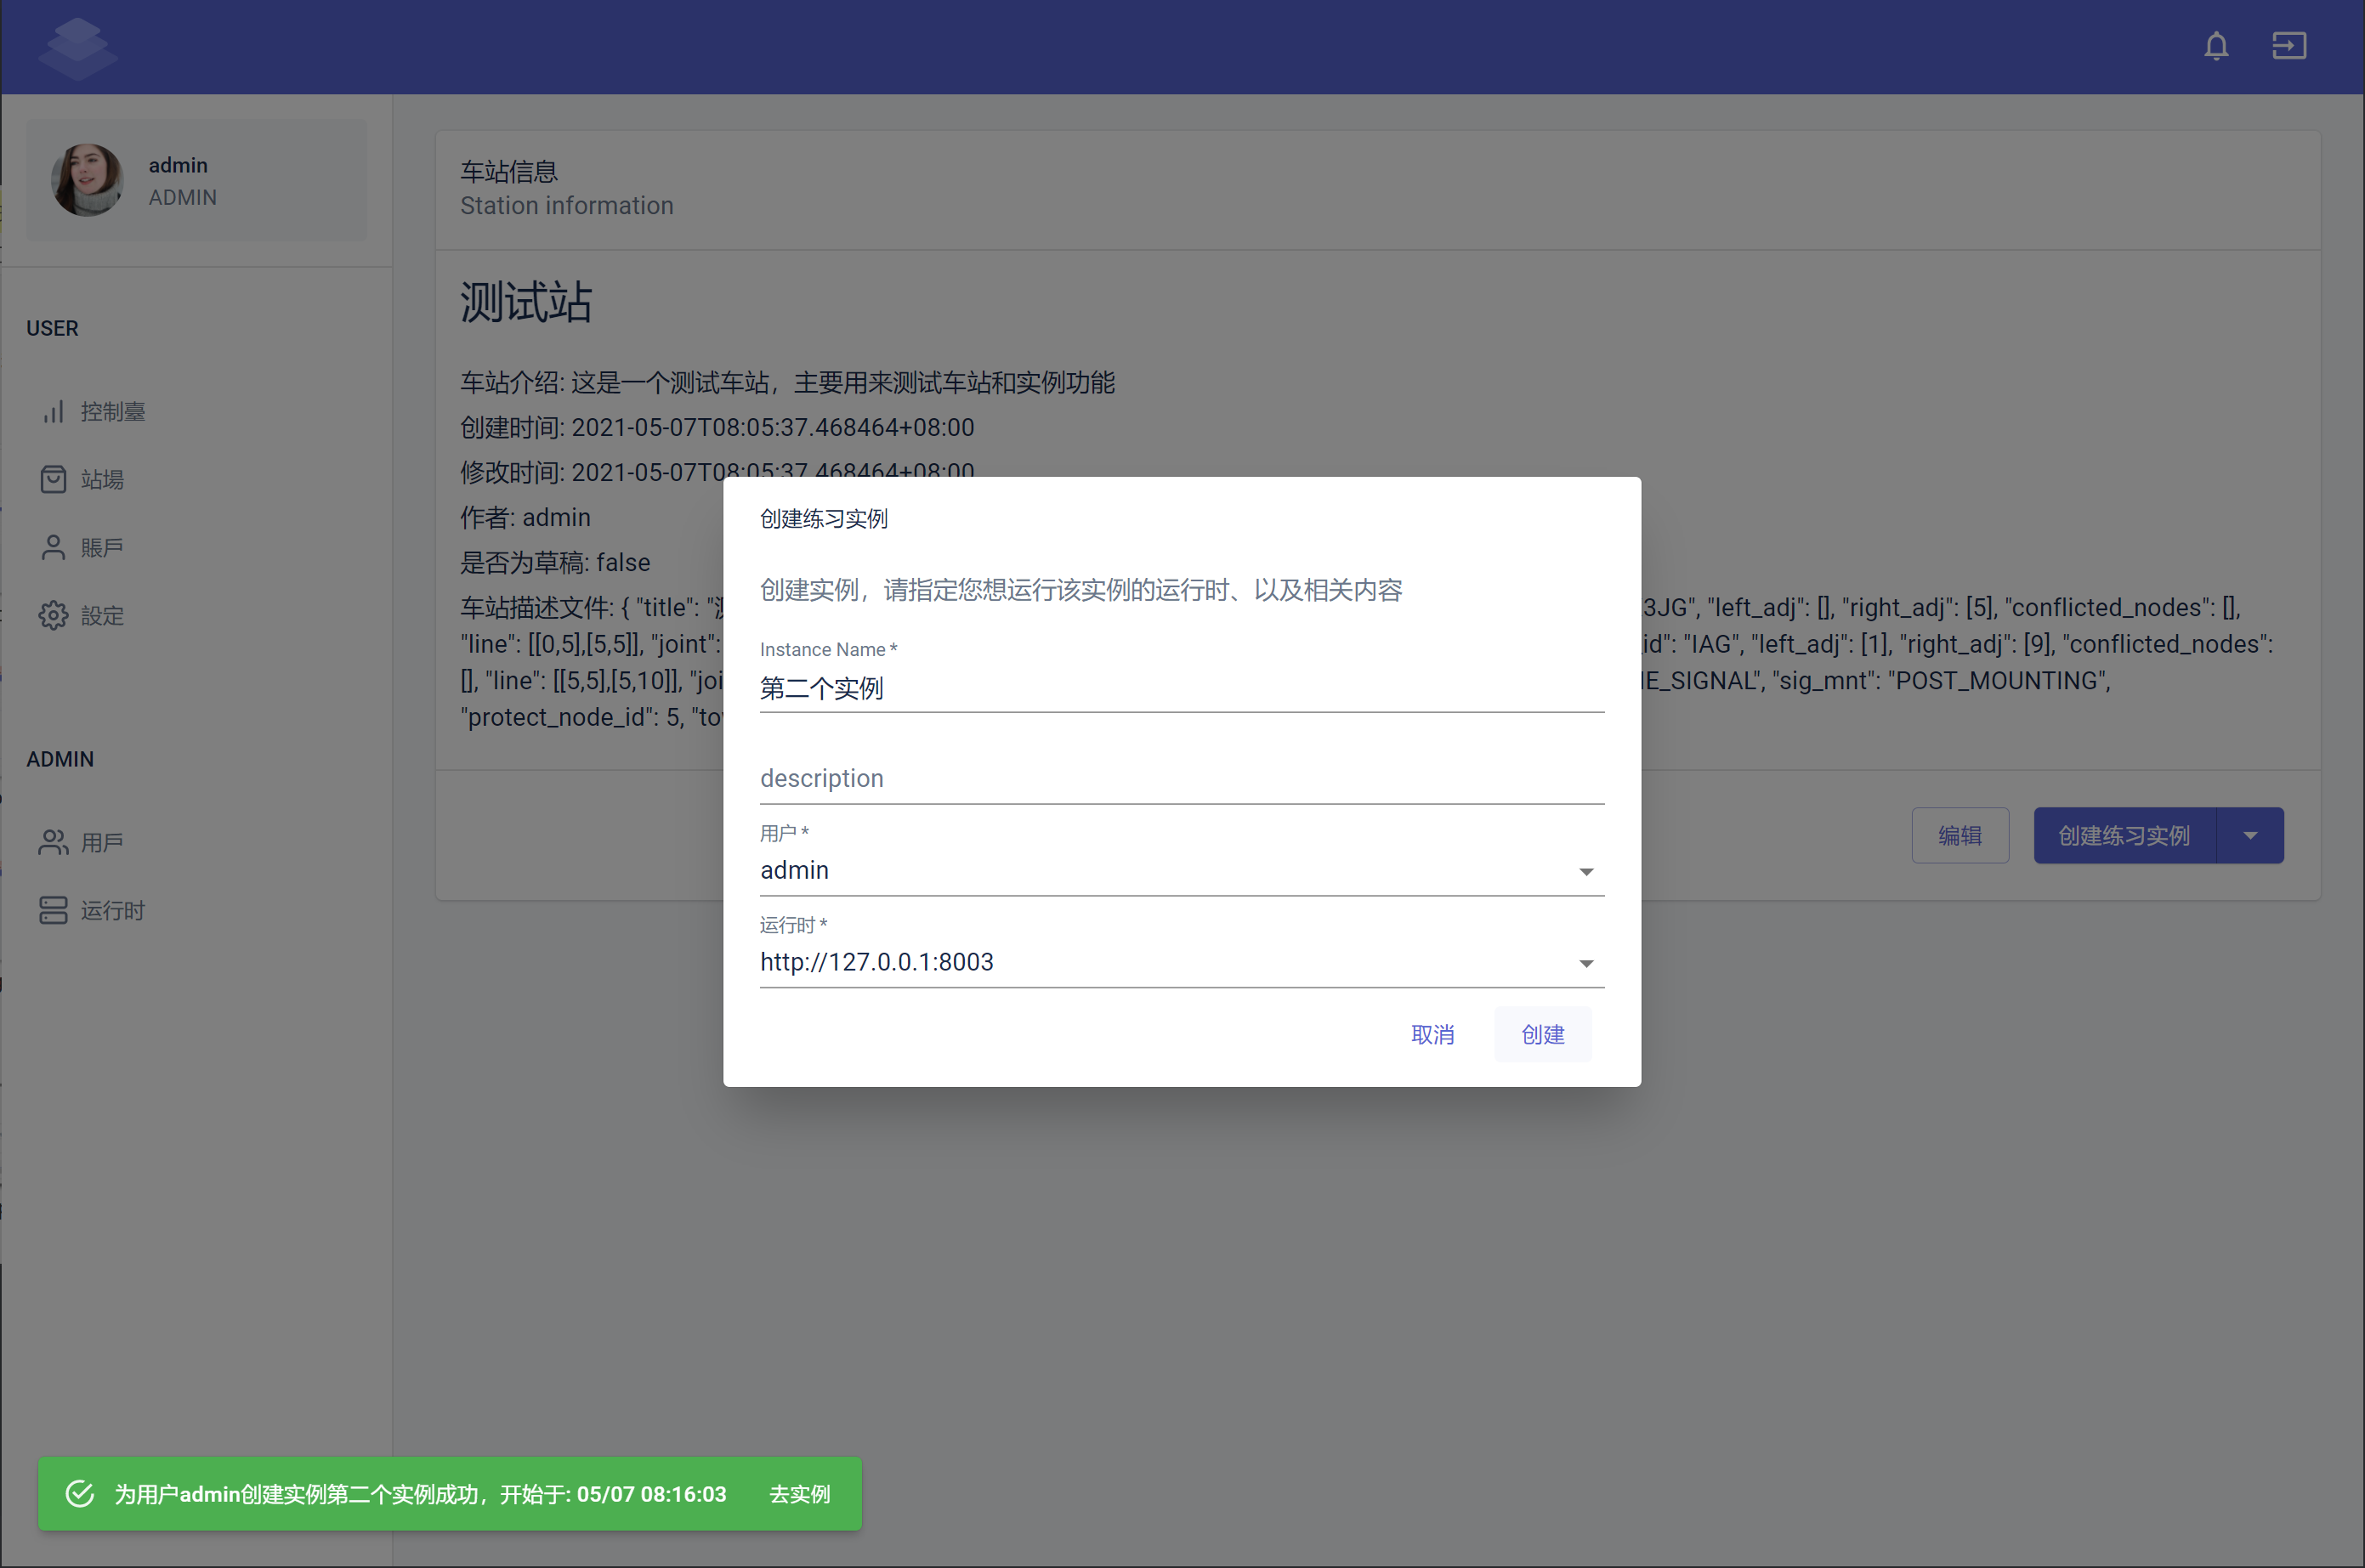
\includegraphics[width=\textwidth]{figures/png/dialog_succ.png}
  \caption{\label{dialog_succ}创建实例成功}
\end{figure}

若新家实例成功,如图\ref{dialog_succ} 所示,
系统会提供用户访问实例的捷径,点击按钮就可以直接访问实例。

\begin{figure}[htbp!]
  \centering
  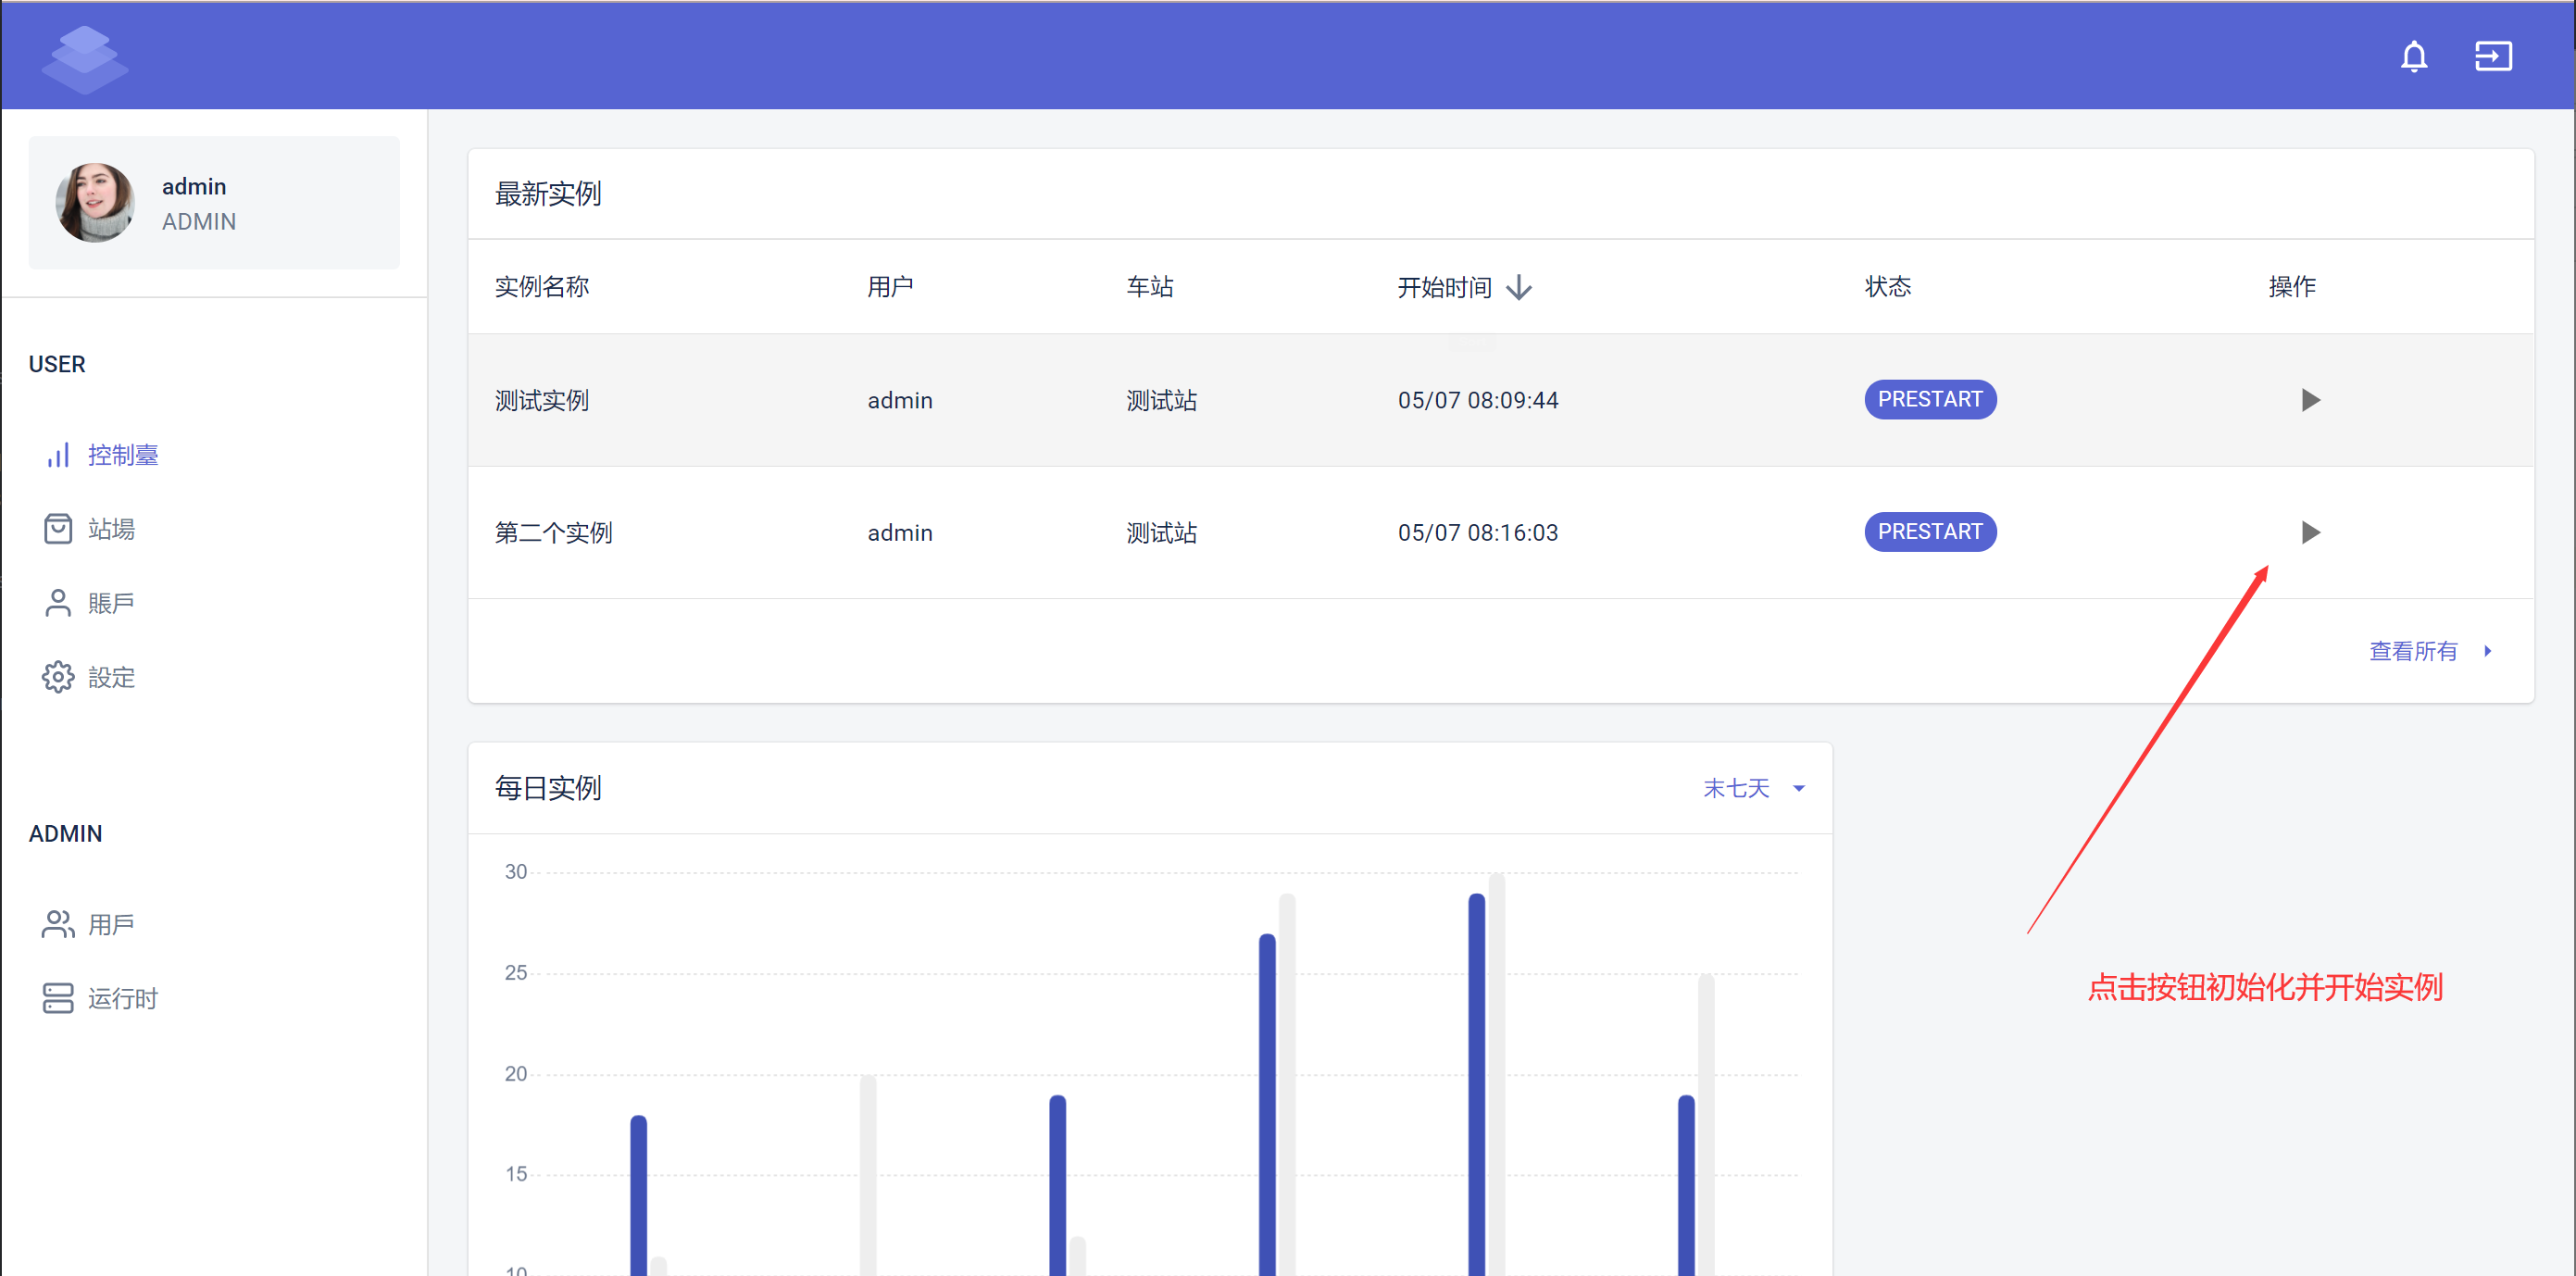
\includegraphics[width=\textwidth]{figures/png/after_create.png}
  \caption{\label{after_create}创建实例后运行实例前}
\end{figure}


\begin{figure}[htbp!]
  \centering
  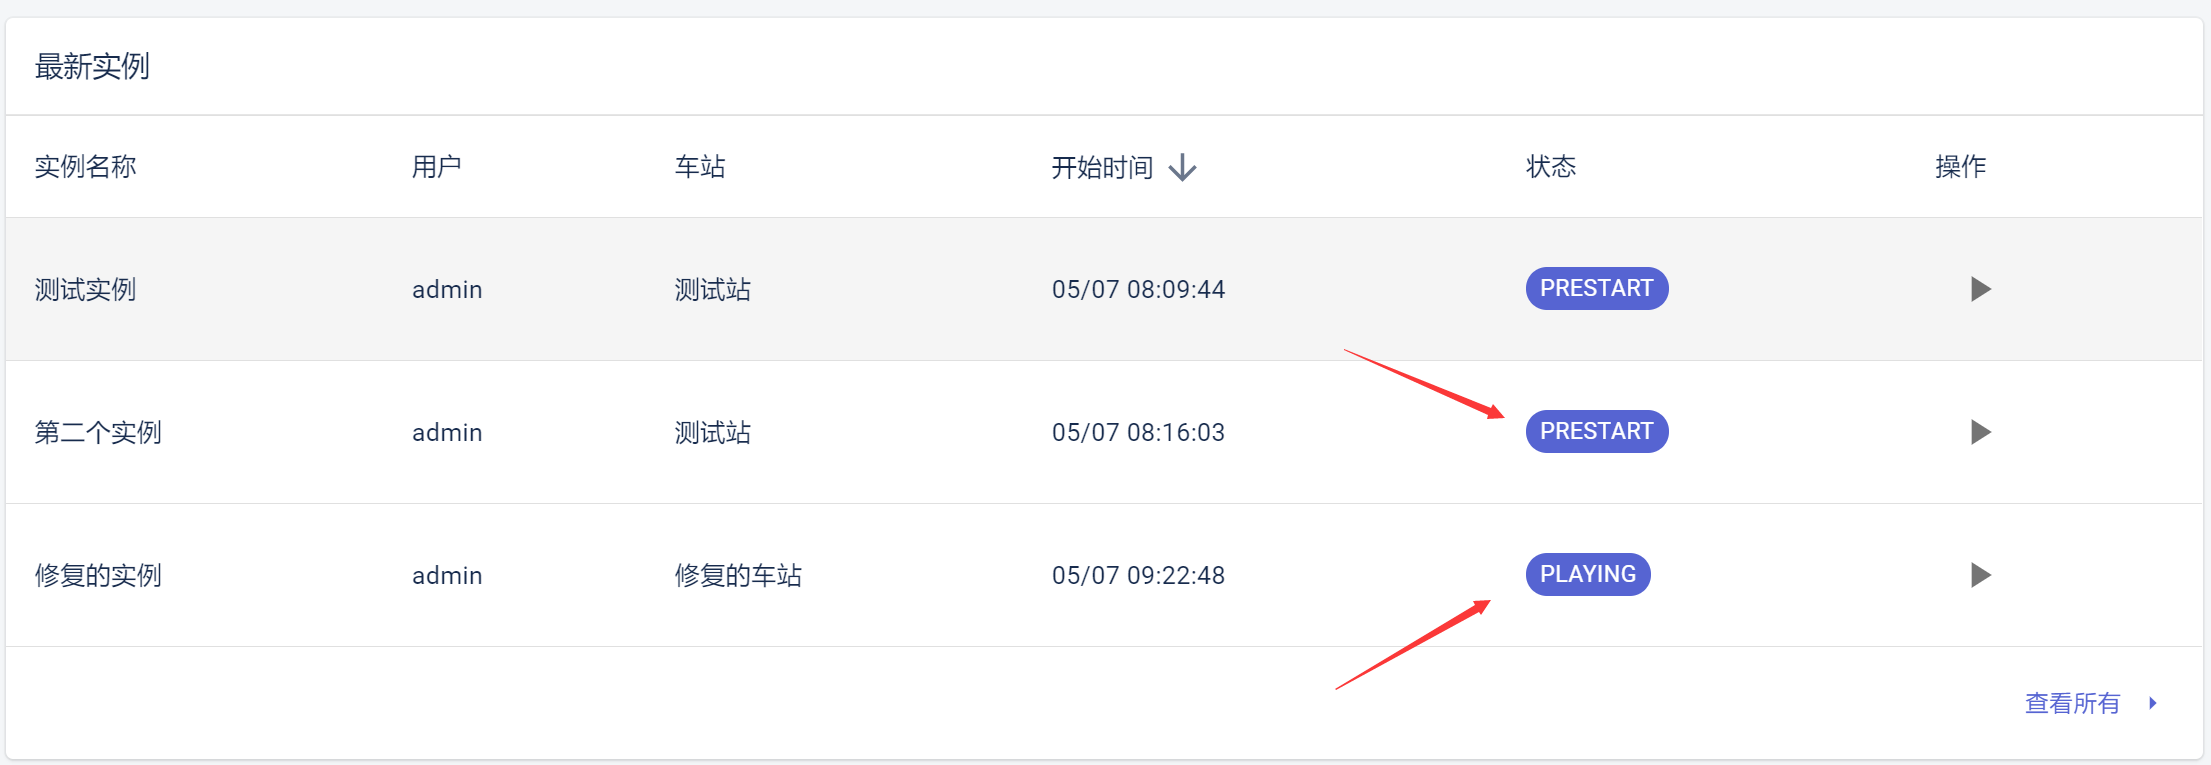
\includegraphics[width=\textwidth]{figures/png/3rd.png}
  \caption{\label{3rd}运行实例后}
\end{figure}

在图 \ref{after_create} 和 \ref{3rd}  中,若当前时间未满开始时间,
则开始的三角按钮不能被按下(图中未体现),也就是前文所述的双重保证。在按下开始按钮后,实例在运行时中被
初始化、运行、实例状态从 PRESTART 变为 PLAYING。表现层的网页
则跳转至实例界面。

% \subsection{实例界面}


%------------结论与致谢----------------%
\begin{keturon}
    在本次设计中,因为工程量大,不可避免遇到了几个预料之外的问题。
    在多线程编程中,为了避免多个线程同时访问资源形成竞态条件,
    通常使用互斥锁(Mutex)来解决问题(本次设计使用的是异步编程,但是
    启用线程池的异步编程)。即当一个线程访问资源时为互斥锁上锁,如果
    互斥锁已经被锁则阻塞该线程,直至互斥锁被解锁,该线程再上锁继续程序。

    这种设计能保证同一时间某个资源至多只有一个线程对其存取,从而避免竞险。
    但是,本案不仅是多线程程序,还是异步程序。因此同步互斥锁是不能够使用
    的,在查询文档后,使用了tokio提供的异步锁。如果第二个线程尝试上异步锁
    则会被挂起。

    因为 Rust 所有权的设计和强制RAII的特性,当 MutexGuard(即被互斥锁保护的资源
    在上锁后得到的句柄)离开作用域后,其drop函数会被调用,互斥锁会被自动解锁。
    所以在在函数调用栈很长的时候会不经意间为同一个资源上两次锁,这样会导致死锁
    的发生。当调试时发现最初的代码有不少死锁的问题。
    在任何编程语言中,避免死锁都是十分需要注意的。

    展望:

    \paragraph{} 当前使用JSON对于用户仍然具有一定的学习成本,
    如果能支持对于车站描述文件的图形化编辑,并且提供实时的车站布局画面预览
    ,将进一步提升用户体验。

    另外,在用户提交车站描述文件后,应当对车站描述文件
    做一次有效性验证,以避免用户输入的信息导致运行时崩溃或生成的实例不可用。
    车站有效性验证应包含如下几项内容:
    \begin{enumerate}
        \item 无垂悬引用 (严格)
        \item 判断$R$图没有孤立点(不严格)
        \item $R$,$S$关系的对称性验证,($S$严格,$R$不严格)
        \item 验证道岔区段组第一性质定理(严格)
        \item 验证每个结点的度(严格)
    \end{enumerate}
    只有严格项目满足,用户输入的车站描述文件才能视之为合法的车站。可以满足
    实例所需要的种种拓扑关系。而不严格项目说明不会产生致命的错误,但显然不是
    现实中合理的车站。因此对用户输入中违反严格项时返回错误,违反非严格项
    时返回警告。

    因为时间关系,本案未能依上述设计对用户的输入进行初步检查。


    \paragraph{} 目前为实现热插拔,没有在运行时使用网关,在表现层通过实例配置时指定的
    运行时创建对应运行时服务的Apollo客户端,从而实现在指定的运行时上运行实例。
    本案的原初设计是在api服务中集成实例调度器(Instance Scheduler),
    其具体职能是管理调度安排实例
    运行在哪个运行时上,还可以将多个运行时视为一种计算“资源”,
    将多个运行时服务池化称为运行时池,通过池中各个运行时的
    负载(运行实例数量、CPU负责、网络IO)等参数来决策新开始的实例应该由哪个运行时
    来运行。调度器通过tarpc(Google 开发的一个Rust专用的rpc专案)和各个运行时连接
    各个运行时作为tarpc服务器,调度器作为tarpc客户端。调度器在某个实例开始时间到时
    通过tarpc服务将新建实例配置传送给一个运行时以运行。
    但是十分遗憾的是,在开发完成调试程序时,发现tarpc要求异步库tokio的最低版本是1.0,
    而本案使用的web 异步框架
    actix-web(latest release)使用tokio版本是0.3,因为异步运行时的版本不兼容,
    导致tarpc与actix-web不能集成于一个项目中。当时我寻求actix-web的替代品,但是
    本案的设计宗旨就是高性能,因为垂涎于actix-web的效率,实在不忍心将actix-web替换为
    别的web框架。因此便舍去了调度器方案。

    在此之后,我又尝试使用redis或者etcd等方案来实现,奈何时间过于紧迫,没添加一项新
    流程、新技术,都意味着阅读学习其使用文档说明、配置环境、处理和现有架构的耦合等等问题,
    要花费的时间不可估算(字面上的意思)。因此最终还是舍弃了使用redis或etcd的方案。
    随着actix-web的更新(actix-web的4.0.x beta版已经使用tokio 1.0了)再将调度器加入api服务中
    就可以了。

\end{keturon}
\begin{arigatou}
    能够完成本次毕业设计,首先要感谢开发过程中使用到的开源项目:

    Mozilla 的 Rust 程序设计语言;

    Facebook 的 GraphQL 和 React.js;

    jonobr1 的 Two.js:面向现代浏览器的二维绘图api;

    Apollo 的 GraphQL 网关和客户端实现;

    Microsoft 的 TypeScript 程序设计语言;

    PostgreSQL Global Development Group的PostgreSQL数据库管理系统;

    Tokio:Rust异步运行时;

    petgraph:Rust 图论算数据结构库;

    Actix Team 的 actix-web:高性能的异步Rust web框架;

    sunli829 的 Async-GraphQL:Rust的异步 GraphQL 服务端实现;

    Diesel Core Team 的 diesel:Rust 的SQL数据库ORM库;

    sfackler 的 r2d2:Rust 的通用数据库连接池;

    OpenJS 基金会的 Node.js:前端web服务器的运行时环境;

    Keats 的 rust-bcrypt:Rust的bcrypt加密算法库;

    Material-UI 的控制台模板。

    若无上述开源项目,本项目便不会存在。

    在使用上述项目时偶尔会遇到一些问题、但作者都会十分热心的解答我的问题,修复项目的bug。
    我由衷的感谢他们。另外感谢\hologo{LuaLaTeX} 、\CTeX 宏包,因此能够便捷地对中文论文进行排版,
    tikz 宏包使我能够绘出本文中的各种图,\hologo{BibTeX} 和 gbt7714 宏包能让我便捷地做出
    符合规范的参考文献。

    就计算机联锁,要感谢尚庆松老师。尚老师传授了的相关知识给我、为毕业设计提供指导意见并
    斧正本文,匡益实多。

    言虽如此,张睿不佞,弇陋不文,是非然否,不敢固也,遑论致谢?
    求早日付梓而所论谫疏,愧诸君相助也。
\end{arigatou}

%-------------参考文献----------------%
\clearpage\null
\bibliographystyle{gbt7714-numerical}
{
    \leading{18pt}
    \bibliography{main}
}
\addcontentsline{toc}{section}{参考文献}

\appendix
%------------附录 -------------------%
\clearpage
\section{相关代码}
\subsection*{客户端schema}
\lstinputlisting{codes/schema.js}

\end{document}